\documentclass[11pt,a4paper]{article}

% --- Packages ---
\usepackage[utf8]{inputenc}
\usepackage[T1]{fontenc}
\usepackage[english]{babel}
\usepackage{amsmath,amssymb,amsfonts,amsthm}
\usepackage{geometry}
\geometry{margin=1in}
\usepackage{graphicx}
\usepackage{hyperref}
\usepackage{xcolor}
\usepackage{cite}
\usepackage{booktabs}
\usepackage{microtype}
\usepackage{physics}
\usepackage{tikz}
\usetikzlibrary{arrows.meta}

\usepackage{listings}

\hypersetup{
    pdftitle={Unified Contraction Hypothesis and Scale-Time Calculus: A Comprehensive Geometric Treatise on Cosmology, Gravitation, and the Four Fundamental Interactions in a Non-Expanding Universe},
    pdfauthor={Muhammed Furkan Haydari},
    pdfsubject={Theoretical Physics, Natural Philosophy, Cosmology and Gravitation},
    pdfkeywords={Unified Contraction Hypothesis, Scale-Time Calculus, Conformal Cosmology, River Model, Fine-Structure Constant 137, Quark Confinement, CMB, Pantheon+},
    colorlinks=true,
    linkcolor=blue!70!black,
    citecolor=red!70!black,
    urlcolor=blue!80!black
}

% --- Listings Settings for Python Code ---
\definecolor{codegreen}{rgb}{0,0.55,0.2}
\definecolor{codegray}{rgb}{0.45,0.45,0.45}
\definecolor{codepurple}{rgb}{0.55,0.1,0.75}
\definecolor{codeblue}{rgb}{0.1,0.2,0.8}
\definecolor{backcolour}{rgb}{0.97,0.97,0.98}

\lstdefinestyle{pythoncode}{
    backgroundcolor=\color{backcolour},   
    commentstyle=\color{codegreen}\itshape,
    keywordstyle=\color{codeblue}\bfseries,
    numberstyle=\tiny\color{codegray},
    stringstyle=\color{codepurple},
    basicstyle=\ttfamily\scriptsize,
    breakatwhitespace=false,         
    breaklines=true,                 
    captionpos=b,                    
    keepspaces=true,                 
    numbers=left,                    
    numbersep=6pt,                  
    showspaces=false,                
    showstringspaces=false,
    showtabs=false,                  
    tabsize=2,
    frame=single,
    rulecolor=\color{gray!30},
    extendedchars=true,
    literate={ğ}{{\u{g}}}1 {ü}{{\"{u}}}1 {ş}{{\c{s}}}1 {ı}{{\i}}1 {ö}{{\"{o}}}1 {ç}{{\c{c}}}1
             {Ğ}{{\u{G}}}1 {Ü}{{\"{U}}}1 {Ş}{{\c{S}}}1 {İ}{{\.I}}1 {Ö}{{\"{O}}}1 {Ç}{{\c{C}}}1
             {²}{{$^2$}}1 {±}{{$\pm$}}1 {χ}{{$\chi$}}1 {Ω}{{$\Omega$}}1 {Λ}{{$\Lambda$}}1 {μ}{{$\mu$}}1 {ℓ}{{$\ell$}}1 {ϕ}{{$\phi$}}1
}
\lstset{style=pythoncode}

% --- Theorem Environments ---
\newtheorem{theorem}{Theorem}[section]
\newtheorem{definition}{Definition}[section]
\newtheorem{axiom}{Axiom}[section]
\newtheorem{corollary}{Corollary}[theorem]
\newtheorem{lemma}[theorem]{Lemma}
\newtheorem{remark}{Remark}[section]

\title{\textbf{Unified Contraction Hypothesis and Scale-Time Calculus: \\ A Comprehensive Geometric Treatise on Cosmology, Gravitation, and the Four Fundamental Interactions in a Non-Expanding Universe}}

\author{
    \textbf{Muhammed Furkan Haydari} \\
    \textit{Independent Research / Conceptual Essays on Natural Philosophy and Fundamental Physics} \\
    \small ORCID: \href{https://orcid.org/0009-0003-2854-3947}{0009-0003-2854-3947}
}

\date{\today}

\begin{document}

\maketitle

\begin{abstract}
    In this treatise, we propose a unified geometric framework that reformulates the four fundamental interactions of nature via the scale dynamics of localized matter embedded in a static, non-expanding background spacetime. Within this \textit{Unified Contraction Hypothesis}, cosmological redshift is derived not as metric stretching of space, but as the direct manifestation of a continuous, scale-conformal shrinkage of local atomic structures ($r_{\mathrm{atom}}(t) \to 0$) relative to the invariant Euclidean background. Through conformal transformations, we demonstrate that this intrinsic atomic shrinkage accounts for the cosmological redshift and time dilation of distant celestial sources without requiring cosmic expansion or dark energy.

    Extending this contraction mechanism to spatial field gradients, we demonstrate that the scale contraction of localized mass-energy continuously draws the surrounding stationary vacuum fabric inward, inducing an effective velocity field. In the macroscopic limit, this vacuum inflow reproduces the Painlev\'e--Gullstrand formulation of general-relativistic gravitation; gravitational acceleration, orbital geodesics, and event horizon light trapping emerge naturally where the inflow velocity reaches $c$. At sub-atomic scales, the classical dilemma of orbital electron collapse is resolved through a scale-invariant conformal attractor: as an electron spirals inward, local length scales contract proportionally ($\mathbb{D}_t(r/\lambda) = 0$), preserving dynamic equilibrium without radiative runaway.

    Finally, we analyze the foundations of electrodynamics and photon propagation. Electromagnetic excitations represent stationary wave perturbations of the invariant background manifold, while the observed speed of light $c = 1/\sqrt{\varepsilon_0\mu_0}$ quantifies the elastic phase velocity of the vacuum fabric. Formalizing wave reflection, scattering, and spectral perception within a contracting observer reference frame, we provide a complete roadmap unifying gravitational, electromagnetic, strong, and weak interactions under a single geometric scale calculus.
\end{abstract}

\vspace{1em}
\noindent\textbf{Keywords:} Unified Field Theory, Conformal Gravity, Contracting Matter Cosmology, Cosmological Redshift, Painlev\'e--Gullstrand Metric, Wave Mechanics, Stationary Vacuum Electrodynamics.

\vspace{1em}
\hrule
\vspace{0.8em}
\tableofcontents
\vspace{0.8em}
\hrule
\vspace{1.5em}

% --- Modular Sections ---
\section*{Epistemological Manifesto: Paradigm Shift and Natural Philosophy}
\addcontentsline{toc}{section}{Epistemological Manifesto: Paradigm Shift and Natural Philosophy}
\label{sec:epistemolojik_manifest}

\subsection*{1. Epistemological Parsimony and the Conformal Geometric Perspective}

The foundational questions encountered in modern theoretical physics and cosmology—such as the nature of dark matter, dark energy, cosmic inflation, and the interface between gravity and quantum scales—motivate the exploration of alternative geometric formulations:
\begin{itemize}
    \item Galactic rotation curves diverging from Keplerian dynamics led to the postulation of cold dark matter.
    \item Distance-redshift relations of Type Ia supernovae led to the hypothesis of dark energy and cosmic acceleration.
    \item Horizon and flatness puzzles motivated cosmic inflation models in the early universe.
    \item Mass generation and confinement problems in field theory continue to stimulate active non-perturbative investigation.
\end{itemize}

This treatise investigates a conformal framework wherein, rather than metric spatial expansion, local atomic and nuclear length standards undergo secular conformal contraction ($r_{\mathrm{atom}}(t) \to 0$) against a static Euclidean background ($\mathcal{E}_\infty$). In the spirit of epistemological parsimony and Occam's razor, our objective is to examine how far scale-covariant differential geometry and conformal duality can account for observed phenomena with minimal axiomatic overhead, offering an exploratory geometric perspective on open cosmological problems.

\subsection*{2. Mathematical Legitimacy: Conformal Duality and Nilpotent Algebra}

The equivalence between spatial expansion and atomic ruler contraction is not merely an interpretative preference; it is a rigorous theorem of differential geometry. In General Relativity, the conformal transformation of the metric tensor:
\begin{equation}
    g_{\mu\nu} \to \Omega^2(t) g_{\mu\nu}
\end{equation}
establishes an exact geometric isomorphism (\textit{conformal duality}) between coordinate systems. As noted by theorists such as Christof Wetterich (2013), Fred Hoyle, Jayant Narlikar, and Roger Penrose across various contexts, an expanding metric space ($a(t) \propto e^{H_0 t}$) and a static background with contracting atomic rulers ($\lambda(t) \propto e^{-H_0 t}$) generate mathematically identical physical observables.

The dual nilpotent algebra ($\kappa^2 = 0$) and the Scale-Covariant Derivative $\mathbb{D}_t \equiv \frac{d}{dt} + \kappa H_0$ developed in this work elevate this conformal symmetry from a passive coordinate gauge choice into a causal and dynamical physical ontology. While space retains its quiescent Euclidean structure, matter is defined as a dynamic Scalor contracting along its internal phase trajectory.

\subsection*{3. Physical Foundations of Fundamental Constants: $c$ and the Sommerfeld Constant $\alpha$}

Standard physics accepts fundamental dimensional and dimensionless constants as empirical givens fixed at the Big Bang without underlying physical mechanisms:
\begin{itemize}
    \item \textit{``Why is the speed of light approximately $3 \times 10^8\text{ m/s}$, and why does it serve as an impassable velocity ceiling?''}
    \item \textit{``What is the physical meaning of the Sommerfeld fine-structure constant $\alpha$ in atomic kinematics?''}
\end{itemize}

Within our hydro-geometric framework:
\begin{enumerate}
    \item \textbf{The Speed of Light ($c$):} Far from being an arbitrary velocity limit, $c$ is the transverse elastic phase transmission speed of the quiescent vacuum continuum ($v_{\mathrm{phase}} = 1/\sqrt{\varepsilon_0\mu_0} = c$) and the characteristic radial contraction phase ceiling of matter vortices ($v_c = c$).
    \item \textbf{The Fine-Structure Constant ($\alpha \approx 1/137.036$):} Represents the \textbf{geometric vortex pitch ratio} required for an orbital electron to balance centrifugal acceleration against the nucleus's radial contraction phase ceiling ($v_r = v_c = c$) without radiative collapse:
          \begin{equation}
              \alpha \equiv \frac{v_\theta}{v_r} = \frac{v_{\mathrm{Bohr}}}{c} = \frac{e^2}{4\pi\varepsilon_0\hbar c} \approx \frac{1}{137.036}.
          \end{equation}
          The relativistic Dirac threshold ($Z\alpha \to 1$) marks the boundary where tangential orbital velocity reaches the contraction ceiling ($v_\theta = c$), inducing Schwinger vacuum polarization ($e^+ e^-$ production) to stabilize the effective nuclear charge.
\end{enumerate}
Reducing these fundamental parameters to kinematic ratios resolves an enduring ontological puzzle in theoretical physics.

\subsection*{4. Invariance of Dimensionless Ratios and Local Laboratory Tests (Eötvös / MICROSCOPE)}

The compatibility of the Unified Contraction Hypothesis with local high-precision laboratory experiments is guaranteed by the scale-invariance of dimensionless ratios. If atomic length scales contracted independently of mass scaling, satellite experiments like MICROSCOPE and terrestrial Eötvös balances would detect differential accelerations, falsifying the theory.

Because all bound mass states acquire conformal mass synchronously according to $m(t) = m_0 e^{H_0 t}$, the measured ratio of any two laboratory masses remains strictly constant:
\begin{equation}
    \frac{d}{dt} \left( \frac{m_{\mathrm{test}}}{m_{\mathrm{ref}}} \right) = \frac{d}{dt} \left( \frac{m_{1,0} e^{H_0 t}}{m_{2,0} e^{H_0 t}} \right) \equiv 0.
\end{equation}
Similarly, the fine-structure constant $\alpha$ and the proton-to-electron mass ratio $\mu = m_p/m_e$ are time-invariant ($\dot{\alpha}/\alpha = 0, \dot{\mu}/\mu = 0$). This explains why tests of the Weak Equivalence Principle (WEP) confirm the absence of differential acceleration down to $\eta < 10^{-15}$.

\subsection*{5. Unifying Celestial and Terrestrial Dynamics: Virial Decoupling and Ephemerides}

Cosmological models often restrict their scope to intergalactic scales, detached from local Solar System constraints. The Unified Contraction Hypothesis seamlessly connects deep-space phenomenology with local celestial mechanics:
\begin{itemize}
    \item \textbf{Local Virial Decoupling and LLR Measurements:} In gravitationally bound systems dominated by local potential ($\nabla^2\Phi \gg 3H_0^2$), orbits decouple from cosmological background expansion in accordance with the McVittie theorem. The measured $3.82\text{ cm/yr}$ recession of the Moon via Lunar Laser Ranging (LLR) is driven by ocean tidal friction, as confirmed by satellite altimetry (TOPEX/Poseidon).
    \item \textbf{Ephemeris and Radar Telemetry Limits:} Because ruler contraction modulates atomic transition frequencies rather than spatial coordinates, the theory remains strictly compatible with radar telemetry constraints on planetary ephemerides ($< 1.5\text{ cm/yr}$ per AU).
\end{itemize}

\subsection*{6. Conceptual Clarity: ``Vacuum Fluid'' vs. 19th-Century Aether (Emergent Spacetime)}

The terminology employed herein---\textit{vacuum flow}, \textit{vortex}, and \textit{Bernoulli gradient}---must not be conflated with 19th-century mechanical luminiferous aether hypotheses. Classical aether was conceived as a dissipative, particulate substance, a concept decisively refuted by the Michelson--Morley experiment.

Here, the background continuum $\mathcal{E}_\infty$ is a frictionless, non-dissipative, massless, and smooth Euclidean manifold. The vacuum flow induced by contracting matter aligns directly with modern formulations of \textit{Emergent Spacetime} and \textit{Analogue/Acoustic Gravity}. Particles are not rigid spheres suspended in space; they are localized topological vortex solitons within the field continuum.

\subsection*{7. Computational Verification and Open-Source Solvers: Minimal CMB Pipeline}

The analytical framework is accompanied by an open-source, reproducible Python solver package (\texttt{scale-cmb-solver}, available at \href{https://github.com/FurkanHaydari/universe-is-not-expanding}{\texttt{FurkanHaydari/universe-is-not-expanding}}) that models the full Planck 2018 CMB angular power spectrum ($\ell = 2\text{--}2500$):
\begin{enumerate}
    \item \textbf{Planck CMB Angular Power Spectrum Solver:} The solver (\texttt{analysis/cmb\_spectrum\_analysis.py}) incorporates the acoustic standing wave transfer equation of contracting plasma, baryon drag ($R_b \approx 0.058$), the acoustic peak spacing ($\Delta\ell \approx 293.5$), early ISW enhancement, and Silk diffusion damping ($\ell_D \approx 1638.7$). It fits the Planck 2018 temperature anisotropy ($D_\ell^{\mathrm{TT}}$) binned data points with high fidelity, reproducing the first three acoustic peaks at $\ell_1 = 220.9$ (observed: 220.0), $\ell_2 = 518.4$ (observed: 537.5), and $\ell_3 = 820.2$ (observed: 810.8) along with their relative amplitude ratios ($H_1/H_2 = 2.169$, $H_3/H_2 = 0.886$).
    \item \textbf{Deuterium and Primordial Abundances Simulation:} The observed intergalactic deuterium abundance ($D/H \sim 2.5 \times 10^{-5}$) is verified through a multi-component \textit{Astrophysical Nuclear Network Simulator} balancing stellar astration with photodisintegration and spallation yields in the quiescent medium.
\end{enumerate}

\subsection*{8. Sociology of Science and Institutional Resistance}

As Max Planck observed: \textit{``A new scientific truth does not triumph by convincing its opponents and making them see the light, but rather because its opponents eventually die, and a new generation grows up that is familiar with it.''}

The primary obstacle facing this framework is the institutional inertia of established paradigms:
\begin{itemize}
    \item Eliminating dark matter and dark energy challenges extensive research programs and funding allocated over decades.
    \item Replacing the Big Bang ($t=0$) singularity with an asymptotic contraction phase transition necessitates a reevaluation of literature founded on expanding metrics.
\end{itemize}
Accordingly, polemical discourse is set aside in favor of an axiomatic, mathematically complete, and empirically testable physical architecture.

\vspace{1.5em}
\hrule
\vspace{1.5em}

\section{Introduction}
\label{sec:giris}

Modern physics rests upon two exceptionally successful yet mutually irreconcilable pillars: General Relativity (GR), which geometricizes gravitation as the curvature of pseudo-Riemannian spacetime, and the Standard Model of particle physics, which describes electromagnetic, weak, and strong interactions as gauge theories on flat or curved backgrounds. Despite a century of sustained theoretical effort, the unification of these four fundamental forces under a single mathematical framework remains elusive. Simultaneously, the standard cosmological paradigm ($\Lambda$CDM) presupposes that the universe is undergoing dynamic metric expansion driven by dark energy and an early epoch of cosmic inflation.

In this monograph, we explore an alternative fundamental premise: \textbf{The background spacetime continuum is strictly static and Euclidean; all observed cosmological and gravitational phenomena arise directly from the continuous, scale-dependent contraction of matter.}

The conceptual foundations of this duality lie in the mathematics of conformal transformations (e.g., Wetterich~\cite{wetterich2013}, Hoyle and Narlikar~\cite{hoyle1964}). Under a conformal transformation $g_{\mu\nu} \to \Omega^2(t) \eta_{\mu\nu}$, an expanding Friedmann--Lema\^itre--Robertson--Walker (FLRW) spacetime with constant particle masses can be mapped isomorphically onto a static Minkowski spacetime where particle masses grow monotonically with cosmic time and characteristic quantum length scales (such as the Bohr radius $a_0 = \hbar^2/(m_e e^2)$ and Compton wavelength $\lambda_C = \hbar/(mc)$) contract:
\begin{equation}
      r_{\mathrm{atom}}(t) \propto \frac{1}{m(t)} \propto a(t)^{-1}.
      \label{eq:konformal_olcekleme}
\end{equation}

A crucial methodological distinction must be emphasized: this model must not be confused with the flawed 1930s ``Tired Light'' hypothesis (which posits photon energy degradation in transit) or stationary Bondi--Gold steady-state cosmologies. In the conformal framework, atomic dimensions diverge in the asymptotic past ($t \to -\infty \implies \lambda \to \infty$); matter in that epoch existed as an overlapping, optically thick ($\tau \gg 1$) plasma in local thermodynamic equilibrium (LTE). Consequently, the core thermodynamic successes of $\Lambda$CDM---including the blackbody nature of the Cosmic Microwave Background (CMB) and primordial nucleosynthesis yields---are preserved through conformal duality.

Whereas prior literature has treated this transformation primarily as a formal coordinate equivalence, we elevate matter contraction to an ontological physical principle governing both cosmological scales and local microscopic interactions.

\subsection{Physical Questions and Investigated Geometric Themes}
\label{sec:temel_sorular}

This monograph investigates the following physical questions and research themes within the framework of conformal scale-covariance and contracting measurement standards:

\begin{enumerate}
      \item \textbf{Atomic Ground State Stability:} \\
            While classical electrodynamics predicts radiative collapse via Larmor emission, at short distances the quantum kinetic pressure arising from Heisenberg momentum uncertainty ($E_{\mathrm{kin}} \propto 1/r^2$) balances the attractive Coulomb potential ($-1/r$), creating a stable Bohr ground state. The Scale-Time derivative ($\mathbb{D}_t(r/\lambda) = 0$) demonstrates that this ground state behaves as a conformal attractor under global contraction (Section~\ref{sec:mikroskopik_kararlilik}).

      \item \textbf{Gravitational Potential and Clock Rates:} \\
            When time is parameterized through the internal quantum phase evolution of contracting matter ($dt = -d\ln\lambda/H_0$), the kinetic resistance experienced by stationary clocks in a gravitational inflow ($v(r) = -\sqrt{2GM/r}$) leads directly to gravitational time dilation $d\tau = dt\sqrt{1 - v^2(r)/c^2}$ (Section~\ref{sec:buzulme_metrikleri}).

      \item \textbf{The Fine-Structure Constant $\alpha$ in Atomic Kinematics:} \\
            The dimensionless Sommerfeld coupling $\alpha \approx 1/137.036$ represents the \textbf{kinematic spiral pitch ratio} between the electron's tangential Bohr orbital velocity ($v_\theta \approx 2187\text{ km/s}$) and the phase transmission ceiling ($v_c = c$): $\alpha = v_{\mathrm{Bohr}} / v_c$. The relativistic Dirac limit ($Z\alpha \to 1$) corresponds to the threshold where tangential orbital velocity approaches $c$, inducing Schwinger pair creation to shield supercritical charge (Section~\ref{sec:olcek_kalkulusu_ana}).

      \item \textbf{Differential Origin of the Hubble Relation ($v = H_0 d$):} \\
            The relation $v = H_0 d$ emerges in static Euclidean coordinates when the Leibniz product rule $[(f\cdot g)' = f'g + fg']$ is applied to a secularly contracting measurement ruler. Observed recessional velocities can thus be interpreted as a kinematic consequence of shrinking standards rather than space expansion (Section~\ref{sec:olcek_kalkulusu_ana}).

      \item \textbf{Cosmic Microwave Background (CMB, 2.73 K) and Thermal History:} \\
            In early epochs with large atomic scales, matter existed as an optically thick ($\tau \gg 1$) plasma. Pre-recombination acoustic standing waves and Kompaneets equilibration produce thermal radiation that, observed with accelerated modern atomic standards, appears as a $2.73\text{ K}$ blackbody spectrum (Section~\ref{sec:cmb_karanlik_madde}).

      \item \textbf{Quantum Phase Pinning and Interferometry:} \\
            Treating photons as transverse elastic phase waves across the vacuum continuum, measurement is modeled as the inelastic phase-pinning of the wavefront to a detector's atomic scale ($\hat{\mathcal{P}}_\kappa$). Delayed-choice erasers~\cite{scully1982,kim2000} recombine separated orthogonal phases, restoring spatial interference fringes (Section~\ref{sec:kuantum_olcum_main}).

      \item \textbf{Hadronic Scale and Quark Confinement:} \\
            At femtometer scales ($r \sim 10^{-15}\text{ m}$), vacuum inflow transitions from spherical dilution to a 1D cylindrical flux tube regime, maintaining an invariant string tension ($\sigma \approx 1\text{ GeV/fm}$) yielding the linear Cornell potential $V(r) = \sigma r$ (Section~\ref{sec:nukleer_kuvvetler}).

      \item \textbf{Dimensional Flow Regimes of Interactions:} \\
            The radial behaviors of gravitational, Coulomb, hadronic, and weak potentials are comparatively examined as effective geometric regimes characterized by dimensional index $\gamma$ within $(v/c)^2 = 2\mathcal{C}r^{-\gamma}$ (Section~\ref{sec:nukleer_kuvvetler}).

      \item \textbf{Chiral Scaling and Baryon Asymmetry:} \\
            The unidirectional scale parameter evolution ($\dot{\lambda} < 0$) establishes an arrow of time ($dt = -d\ln\lambda/H_0$), providing a dynamic framework to investigate chiral symmetry breaking where right-handed matter vortex states achieve stable nuclear confinement (Section~\ref{sec:olcek_kalkulusu_ana}).

      \item \textbf{Parametric Interconnection of Foundational Quantities:} \\
            Investigating how time ($t$), position ($\mathbf{x}$), mass ($m$), and phase propagation speed ($c$) can be self-consistently interrelated through the scalar scale parameter $\lambda(t)$ and scale-time calculus (Section~\ref{sec:ontolojik_indirgeme}).
\end{enumerate}

\subsection{Ontological Necessity: Unifying the Four Primitives}
\label{sec:ontolojik_indirgeme}

Standard theoretical physics treats its four foundational building blocks as disconnected postulates:
\begin{enumerate}
      \item \textbf{Time ($t$):} An independent coordinate axis or an external parameter along which quantum states evolve.
      \item \textbf{Space ($\mathbf{x}$):} A Riemannian background manifold or an arena supporting quantum fields.
      \item \textbf{Mass ($m, M$):} An inertial coefficient assigned externally or acquired via arbitrary Yukawa couplings in the Higgs mechanism.
      \item \textbf{Speed of Light ($c$):} An invariant causality boundary postulated without mechanical justification.
\end{enumerate}

As long as these quantities remain isolated primitives, unifying their derived force fields is epistemologically impossible. In the Unified Contraction Hypothesis, all four quantities are derived from \textbf{the Scale Evolution of Matter in Quiescent Vacuum ($\lambda(t)$ and $\kappa$)}:
\begin{itemize}
      \item \textbf{Speed of Light ($c$):} The transverse elastic wave propagation speed in quiescent vacuum, identical to the internal quantum phase ceiling of matter vortices ($v_c = 1/\sqrt{\varepsilon_0\mu_0} = c$).
      \item \textbf{Time ($t$):} The logarithmic quantum phase log recorded by contracting atomic clocks ($dt \equiv -\frac{1}{H_0} d\ln\lambda$).
      \item \textbf{Position / Distance ($R$):} The dimensionless ratio between static Euclidean coordinates $\mathbf{X}_0$ and the contracting atomic length standard $\lambda(t)$ ($R(t) = \mathbf{X}_0 / \lambda(t)$).
      \item \textbf{Mass ($M$):} The net Gauss surface flux of vacuum flow acceleration ($M \equiv \frac{1}{4\pi G} \oint_{\partial \Omega} |(\mathbf{v}_{\mathrm{inflow}} \cdot \nabla) \mathbf{v}_{\mathrm{inflow}}| \, dA$).
\end{itemize}

Once these four primitives are unified through $\lambda(t)$, the fundamental forces cease to be distinct fields and emerge as different geometric branches ($(v/c)^2 = 2\mathcal{C}r^{-\gamma}$) of a single vacuum inflow dynamics.

\subsection{Corpus Organization and Companion Preprints}
\label{sec:corpus_organization}

This monograph synthesizes the unified theoretical framework developed across seven dedicated companion research preprints:
\begin{enumerate}
    \item \textbf{Paper I (Cosmology \& Supernova Distance Modulus):} Conformal redshift in a static universe and analytical derivation of the Type Ia supernova distance modulus without dark energy~\cite{haydari_cosmo}.
    \item \textbf{Paper II (Scale-Time Calculus):} Mathematical foundations of scale-time algebra, the nilpotent generator $\kappa$, and conformal calculus for contracting systems~\cite{haydari_calculus}.
    \item \textbf{Paper III (Early Massive Galaxies in JWST):} Conformal angular diameter distances and stellar mass density resolution without anomalous starbursts~\cite{haydari_jwst}.
    \item \textbf{Paper IV (River Model of Gravitation):} Reinterpreting pseudo-Riemannian curved metrics as inflowing vacuum flux across flat Euclidean space~\cite{haydari_gravity}.
    \item \textbf{Paper V (Electromagnetism \& Fine-Structure Constant):} Kinematic derivation of $\alpha^{-1} \approx 137.036$ and quantum measurement dynamics~\cite{haydari_em}.
    \item \textbf{Paper VI (Strong Force \& Hadronic Confinement):} Flux tube saturation geometry, dimensional reduction, and the origin of linear quark confinement~\cite{haydari_strong}.
    \item \textbf{Paper VII (Weak Interaction \& Chiral Torsion):} Geometrizing electroweak symmetry breaking and Fermi scale decay via chiral phase leakage~\cite{haydari_weak}.
\end{enumerate}

\section{Standard Metric Systems in Contemporary Physics}
\label{sec:standart_metrik}

Contemporary theoretical physics employs the metric tensor formalism of pseudo-Riemannian geometry ($g_{\mu\nu}$) to describe spacetime geometry and dynamics. The differential line element is expressed generally as:
\begin{equation}
    ds^2 = g_{\mu\nu} dx^\mu dx^\nu.
    \label{eq:genel_cizgi_elemani}
\end{equation}

Standard physics relies upon three primary metric formulations:

\subsection{Flat Spacetime (The Minkowski Metric)}
In Special Relativity, inertial reference frames devoid of gravitational curvature are described by the Minkowski metric $\eta_{\mu\nu} = \mathrm{diag}(-1, 1, 1, 1)$:
\begin{equation}
    ds^2 = -c^2 dt^2 + dx^2 + dy^2 + dz^2 = -c^2 dt^2 + dr^2 + r^2 d\Omega^2,
    \label{eq:minkowski_metrik}
\end{equation}
where $d\Omega^2 = d\theta^2 + \sin^2\theta d\phi^2$ is the metric on the unit 2-sphere. Here, $c$ is postulated as the invariant propagation velocity of electromagnetic waves in vacuum, and the coordinate grid is assumed strictly rigid and time-independent.

\subsection{Expanding Universe Metric (FLRW)}
In standard $\Lambda$CDM cosmology, assuming spatial homogeneity and isotropy on large scales leads to the Friedmann--Lema\^itre--Robertson--Walker (FLRW) line element:
\begin{equation}
    ds^2 = -c^2 dt^2 + a^2(t) \left[ \frac{dr^2}{1 - kr^2} + r^2 d\Omega^2 \right],
    \label{eq:flrw_metrik}
\end{equation}
where $a(t)$ is the dimensionless cosmic scale factor, and $k \in \{-1, 0, 1\}$ parameterizes spatial curvature. For a spatially flat universe ($k=0$):
\begin{equation}
    ds^2 = -c^2 dt^2 + a^2(t) d\mathbf{x}^2.
    \label{eq:flrw_duz}
\end{equation}
In standard interpretation, the proper physical distance between two co-moving galaxies $R(t) = a(t) r$ expands with cosmic time. The observed redshift ($z$) of distant sources is interpreted as the stretching of photon wavelengths by the expanding metric:
\begin{equation}
    1 + z = \frac{\lambda_{\mathrm{obs}}}{\lambda_{\mathrm{emit}}} = \frac{a(t_0)}{a(t_e)}.
    \label{eq:standart_redshift}
\end{equation}

\subsection{Gravitational Curvature Metrics (Schwarzschild and Painlev\'e--Gullstrand)}
The spacetime exterior to a static, spherically symmetric mass $M$ is conventionally expressed in Schwarzschild coordinates:
\begin{equation}
    ds^2 = -\left(1 - \frac{2GM}{c^2 r}\right) c^2 dt^2 + \left(1 - \frac{2GM}{c^2 r}\right)^{-1} dr^2 + r^2 d\Omega^2.
    \label{eq:schwarzschild_standart}
\end{equation}
Transforming to the proper time of an observer freely falling from rest at infinity ($dt_{\mathrm{ff}} = dt + \frac{\sqrt{2GM/r}}{c(1 - 2GM/c^2 r)} dr$) yields the Painlev\'e--Gullstrand line element~\cite{painleve1921, gullstrand1922}:
\begin{equation}
    ds^2 = -c^2 dt_{\mathrm{ff}}^2 + \left( dr + \sqrt{\frac{2GM}{r}} dt_{\mathrm{ff}} \right)^2 + r^2 d\Omega^2.
    \label{eq:painleve_standart}
\end{equation}
This formulation underpins the ``river model'' of space: the background Euclidean spatial coordinate grid remains stationary, while the vacuum field undergoes a radial inflow toward the center of mass at velocity $v_{\mathrm{inflow}}(r) = \sqrt{2GM/r}$, akin to electric current flowing through a stationary copper lattice.

\section{The Unified Contraction Hypothesis: Contraction Velocity (\texorpdfstring{$v_c$}{vc}) and Metric Reconstruction}
\label{sec:buzulme_metrikleri}

Inverting the standard metric paradigm, we proceed from the premise that space does not expand; rather, matter undergoes scale contraction.

\subsection{The Fundamental Invariant: Contraction Velocity (\texorpdfstring{$v_c$}{vc}) in Lieu of Postulated Light Speed}
In standard physics, the constant $c$ is postulated as the invariant speed of light in vacuum. We state the following fundamental axiom:

\begin{quote}
    \textbf{Axiom 1 (Vacuum Phase Propagation and the Intrinsic Quantum Phase Ceiling of Matter):}
    The static background space and the vacuum continuum are strictly stationary ($\mathbf{v}_{\mathrm{space}} = 0$). Photons are transverse elastic phase stress waves propagating across neighboring cells of this stationary vacuum continuum ($v_{\mathrm{trans}} = 0$). This phase wave propagates across Euclidean space at the characteristic transmission speed of the vacuum: $v_{\mathrm{phase}} = 1/\sqrt{\varepsilon_0\mu_0}$.

    Matter, constituted by closed topological vortex solitons (Scalor knots) in this vacuum, exhibits an intrinsic relativistic quantum phase circulation velocity ceiling ($v_c$) that matches the elastic transmission speed of the medium:
    \begin{equation}
        v_c \equiv \frac{1}{\sqrt{\varepsilon_0\mu_0}} = c \approx 2.99792 \times 10^8 \text{ m/s}.
        \label{eq:buzulme_hizi_tanim}
    \end{equation}
    Two distinct velocity regimes must be carefully distinguished:
    \begin{enumerate}
        \item \textbf{Intrinsic Quantum Phase Velocity ($v_c = c$):} The elastic phase propagation speed of the vacuum and the internal relativistic circulation ceiling of the atomic vortex ($c \approx 3 \times 10^8\text{ m/s}$).
        \item \textbf{Cosmological Scale Contraction Rate ($|\dot{r}_{\mathrm{atom}}| = H_0 r_{\mathrm{atom}}$):} The secular rate at which atomic radii contract ($|\dot{r}_{\mathrm{atom}}| \approx (2.3 \times 10^{-18}\text{ s}^{-1}) \times (10^{-10}\text{ m}) \approx 2.3 \times 10^{-28}\text{ m/s}$). This rate is 36 orders of magnitude ($10^{36}$) smaller than $c$, ensuring atomic stability over billions of years.
    \end{enumerate}
    When measured using contracting atomic rulers and clocks, the propagation speed of this free phase wave is recorded as exactly $c$ relative to our internal phase standard ($v_{\mathrm{phase}} = v_c = c$). Cosmological redshift originates from the secular contraction ($r_{\mathrm{atom}}(t) \to 0$) of the atomic rulers recording this constant-wavelength vacuum oscillation.
\end{quote}

The fundamental line element on the invariant background coordinates ($\mathbf{x}, t$) remains flat:
\begin{equation}
    d\Sigma^2 = -v_c^2 dt^2 + d\mathbf{x}^2.
    \label{eq:statik_arkaplan_metrigi}
\end{equation}

\subsection{Cosmological Metric: Contracting Atomic Standards vs. Expanding Space}
Spatial coordinates $\mathbf{x}$ do not expand ($d\mathbf{x} = \text{const}$). However, all measurement standards (atomic rulers $r_{\mathrm{atom}}$) contract with time. We define the dimensionless atomic scale function:
\begin{equation}
    \lambda(t) \equiv \frac{r_{\mathrm{atom}}(t)}{r_{\mathrm{atom}}(t_0)} = \frac{1}{a(t)}, \quad \lambda(t_0) = 1.
    \label{eq:olcek_fonksiyonu}
\end{equation}
The contraction rate is given by the logarithmic derivative:
\begin{equation}
    \frac{\dot{\lambda}(t)}{\lambda(t)} = -H_0.
    \label{eq:buzulme_hubble}
\end{equation}

The differential length $d\mathbf{x}_{\mathrm{obs}}$ measured by a contracting ruler relates to background coordinate displacement $d\mathbf{x}$ as:
\begin{equation}
    d\mathbf{x}_{\mathrm{obs}} = \frac{d\mathbf{x}}{\lambda(t)} \implies d\mathbf{x} = \lambda(t) d\mathbf{x}_{\mathrm{obs}}.
    \label{eq:cetvel_donusumu}
\end{equation}
Substituting this into the static background metric~\eqref{eq:statik_arkaplan_metrigi}:
\begin{equation}
    d\Sigma^2 = -v_c^2 dt^2 + \lambda^2(t) d\mathbf{x}_{\mathrm{obs}}^2.
    \label{eq:buzulen_cetvel_metrigi}
\end{equation}
For a local observer assuming their contracted ruler to be invariant, the effective metric is obtained by conformal rescaling $ds_{\mathrm{eff}}^2 = \lambda^{-2}(t) d\Sigma^2$:
\begin{equation}
    ds_{\mathrm{eff}}^2 = -\frac{v_c^2}{\lambda^2(t)} dt^2 + d\mathbf{x}_{\mathrm{obs}}^2 = -v_c^2 d\tau^2 + a^2(\tau) d\mathbf{x}_{\mathrm{static}}^2,
    \label{eq:etkin_flrw}
\end{equation}
where $d\tau = \lambda^{-1}(t) dt = a(t) dt$ is the conformal cosmological time.

\textbf{Mathematical Conclusion:} The FLRW metric of standard $\Lambda$CDM cosmology is the exact conformal projection of contracting atomic rulers in a static Minkowski space. Redshift ($z$) reflects the lower transition frequencies of larger atoms in the past ($t_e$):
\begin{equation}
    1 + z = \frac{\nu_{\mathrm{ref}}}{\nu_{\mathrm{obs}}} = \frac{m(t_0)}{m(t_e)} = \frac{r_{\mathrm{atom}}(t_e)}{r_{\mathrm{atom}}(t_0)} = \frac{\lambda(t_e)}{\lambda(t_0)}.
    \label{eq:bizim_redshift}
\end{equation}

\subsection{Gravitational Vacuum-Inflow Metric and Continuity Equation}
A mass $M$ is a localized concentration of contracting atomic vortices. The continuous contraction of matter draws an inward vacuum flux (inflow velocity field) from the surrounding stationary continuum.

\subsubsection{Variational Derivation: 3+1 ADM Action and River Velocity in Flat Space}
\label{sec:adm_eylem_turetilis}
The vacuum inflow velocity $v(r) = -\sqrt{2GM/r}$ in the River Model is the **exact variational Euler--Lagrange solution of the Einstein--Hilbert action subject to a flat Euclidean spatial constraint.**

In the Arnowitt--Deser--Misner (ADM) 3+1 decomposition, the metric is:
\begin{equation}
    ds^2 = -\left(N^2 - \beta_i \beta^i\right) v_c^2 dt^2 + 2 \beta_i v_c dt dx^i + \gamma_{ij} dx^i dx^j,
    \label{eq:adm_metrik_ayrisim}
\end{equation}
where $N$ is the lapse, $\boldsymbol{\beta}$ is the shift vector, and $\gamma_{ij}$ is the spatial 3-metric.

Constraining the spatial slice to a flat Euclidean continuum with uniform coordinate time slicing:
\begin{equation}
    \gamma_{ij} = \delta_{ij} \quad (\text{Flat Euclidean Space}, \; R^{(3)} = 0), \qquad N = 1 \quad (\text{Uniform Time Slicing}).
    \label{eq:duz_uzay_kisit}
\end{equation}
The sole dynamical degree of freedom of the gravitational field is the shift vector:
\begin{equation}
    \boldsymbol{\beta}(\mathbf{r}) \equiv -\frac{\mathbf{v}_{\mathrm{vacuum}}(\mathbf{r})}{v_c}.
    \label{eq:shift_vektor_tanim}
\end{equation}
The extrinsic curvature tensor is given by:
\begin{equation}
    K_{ij} \equiv \frac{1}{2N} \left( \nabla_i \beta_j + \nabla_j \beta_i \right) = -\frac{1}{2 v_c} \left( \partial_i v_j + \partial_j v_i \right), \qquad K \equiv K^i_i = -\frac{1}{v_c} \nabla \cdot \mathbf{v}.
    \label{eq:dissal_egrilik_shift}
\end{equation}

Under the flat-space constraint, the Einstein--Hilbert action $S_{\mathrm{EH}} = \frac{v_c^3}{16\pi G} \int d^4x \sqrt{-g} R$ reduces to:
\begin{equation}
    S_{\mathrm{grav}}[\mathbf{v}] = \frac{v_c^3}{16\pi G} \int dt d^3x \left( K_{ij} K^{ij} - K^2 \right) + S_{\mathrm{matter}}[\mathbf{v}].
    \label{eq:adm_grav_eylem}
\end{equation}
For a spherically symmetric, stationary radial flow ($\mathbf{v} = v(r) \hat{\mathbf{r}}$), the extrinsic curvature components are:
\begin{equation}
    K_{rr} = -\frac{1}{v_c} \frac{dv}{dr}, \qquad K_{\theta\theta} = K_{\phi\phi} = -\frac{1}{v_c} \frac{v(r)}{r},
\end{equation}
yielding the kinetic curvature scalar:
\begin{equation}
    K_{ij} K^{ij} - K^2 = -\frac{2}{v_c^2} \left( \frac{v}{r} \frac{dv}{dr} + \frac{v^2}{r^2} \right) = -\frac{1}{v_c^2 r^2} \frac{d}{dr}\left( r v^2 \right).
    \label{eq:kinetik_egrilik_ozdeslik}
\end{equation}
Varying the total action with respect to $v(r)$ for a point mass $M$ at rest ($\delta S / \delta v(r) = 0$):
\begin{equation}
    \frac{\delta S_{\mathrm{grav}}}{\delta v(r)} = 0 \implies \nabla \cdot \left( v \frac{dv}{dr} \hat{\mathbf{r}} \right) = -4\pi G M \delta^3(\mathbf{r}) \implies v(r) \frac{dv(r)}{dr} = -\frac{GM}{r^2}.
    \label{eq:varyasyon_akis_sonuc}
\end{equation}
Imposing the asymptotic quiescence condition $v(\infty) = 0$:
\begin{equation}
    \mathbf{v}_{\mathrm{vacuum}}(r) = -\sqrt{\frac{2GM}{r}} \hat{\mathbf{r}}.
    \label{eq:vakum_cekis_hizi}
\end{equation}
This confirms that the Painlevé--Gullstrand velocity field is the unique Euler--Lagrange extremum of the ADM action in flat space.

\subsubsection{Where Does the Vacuum Go? The Nilpotent Sink and Vacuum Divergence}
In classical fluid mechanics, continuous inward flow requires accumulation or an infinite density singularity. Two regimes must be distinguished:
\begin{enumerate}
    \item \textbf{Empty Space Regime ($r > 0, \rho_M = 0$):} The divergence of the velocity field in flat Euclidean space is:
    \begin{equation}
        \nabla \cdot \mathbf{v}_{\mathrm{vacuum}} = -\frac{3}{2} \sqrt{\frac{2GM}{r^3}} = - v_c K.
        \label{eq:extrinsic_curvature_trace}
    \end{equation}
    This divergence does not signify fluid annihilation in vacuum; rather, in the 3+1 ADM decomposition, it corresponds to the trace of the extrinsic curvature of constant-time hypersurfaces ($K \equiv K^i_i = -\frac{1}{v_c}\nabla\cdot\mathbf{v}$), quantifying the rate of coordinate contraction toward the center.
    \item \textbf{Matter Core and Nilpotent Sink ($r \to 0, \rho_M \neq 0$):} At the origin where the flow converges upon matter, the continuity equation is balanced by a nilpotent sink term:
    \begin{equation}
        \nabla \cdot \mathbf{v}_{\mathrm{physical}} = -4\pi G \rho_M \kappa = \mathcal{S}_{\mathrm{sink}}.
        \label{eq:sureklilik_main}
    \end{equation}
    The 3-dimensional vacuum flux entering the center does not accumulate in space. Due to the nilpotency condition $\kappa^2 = 0$, spatial flux is converted into the intrinsic quantum phase frequency ($\omega = M c^2 / \hbar$) and internal scale contraction rate ($\dot{\lambda} = -H_0 \lambda$) of matter. Curvature singularities at $r=0$ are thus resolved as phase-conversion boundaries.
\end{enumerate}

The line element experienced by a test particle or wave in this inflow is:
\begin{equation}
    ds^2 = -v_c^2 dt^2 + \left( dr - v_{\mathrm{vacuum}}(r) dt \right)^2 + r^2 d\Omega^2.
    \label{eq:bizim_vakum_metrigi}
\end{equation}
Expanding the quadratic term:
\begin{equation}
    ds^2 = -\left(1 - \frac{v_{\mathrm{vacuum}}^2(r)}{v_c^2}\right) v_c^2 dt^2 - 2 v_{\mathrm{vacuum}}(r) dt dr + dr^2 + r^2 d\Omega^2.
    \label{eq:vakum_metrik_acik}
\end{equation}
Substituting $v_{\mathrm{vacuum}}(r) = -\sqrt{2GM/r}$:
\begin{equation}
    ds^2 = -\left(1 - \frac{2GM}{v_c^2 r}\right) v_c^2 dt^2 + 2\sqrt{\frac{2GM}{r}} dt dr + dr^2 + r^2 d\Omega^2.
    \label{eq:bizim_yercekimi_tam}
\end{equation}

\paragraph{3D Flat Slices and 4D Riemann Curvature (Gauss--Codazzi Relation):}
Having Euclidean spatial slices ($\gamma_{ij} = \delta_{ij}$, $^{(3)}R \equiv 0$) in Painlevé--Gullstrand coordinates does not imply that spacetime is flat. The full 4D spacetime curvature is generated via the 3+1 ADM Gauss--Codazzi equation ($^{(4)}R = K_{ij}K^{ij} - K^2$) by the extrinsic curvature tensor ($K_{ij} = -\frac{1}{2c}(\partial_i v_j + \partial_j v_i)$). The resulting Kretschmann invariant $\mathcal{K} \equiv R^{\alpha\beta\gamma\delta} R_{\alpha\beta\gamma\delta} = \frac{48 G^2 M^2}{c^4 r^6}$ matches the exact Schwarzschild geometry. Thus, the River Model provides an exact hydrodynamic representation of 4D spacetime curvature as a vacuum velocity gradient on a Euclidean background.

\subsection{Acceleration Mechanism in Vacuum Flow: Convective Acceleration and $g = GM/r^2$}
\label{sec:ivmelenme_ispat}

Why does a falling body continuously accelerate ($g \approx 9.8\text{ m/s}^2$) rather than drifting at a constant velocity in the vacuum stream?

The answer is dictated by Euler convective acceleration in a converging spherical flow:

\subsubsection{1. Spherical Convergence and Escape Velocity}
The spherical shell area is $A(r) = 4\pi r^2$. As vacuum flows toward the center, conservation of energy ($\frac{1}{2} v^2 - \frac{GM}{r} = 0$) dictates that velocity increases monotonically as $r^{-1/2}$:
\begin{equation}
    v_{\mathrm{inflow}}(r) = -\sqrt{\frac{2GM}{r}} \hat{\mathbf{r}}.
\end{equation}
At Earth's surface ($r = R_\oplus \approx 6371\text{ km}$):
\begin{equation}
    |v_{\mathrm{inflow}}(R_\oplus)| = \sqrt{\frac{2GM_\oplus}{R_\oplus}} \approx 11.186\text{ km/s},
\end{equation}
which is exactly Earth's escape velocity.

\subsubsection{2. Euler Convective Acceleration Proof}
In fluid mechanics, the acceleration of a particle in a velocity field is governed by the material derivative:
\begin{equation}
    \mathbf{a} = \frac{D\mathbf{v}}{Dt} = \frac{\partial \mathbf{v}}{\partial t} + (\mathbf{v} \cdot \nabla)\mathbf{v}.
\end{equation}
For a stationary mass, $\partial \mathbf{v}/\partial t = 0$. The convective radial acceleration experienced by a free particle falling through the stream is:
\begin{equation}
    a_r(r) = v(r) \frac{dv(r)}{dr}.
    \label{eq:konvektif_ivme_tanim}
\end{equation}
Evaluating the radial gradient step by step:
\begin{equation}
    a_r(r) = \left( -\sqrt{2GM} \, r^{-1/2} \right) \left( \frac{1}{2} \sqrt{2GM} \, r^{-3/2} \right) = \mathbf{-\frac{GM}{r^2}}.
    \label{eq:g_ispat_sonuc}
\end{equation}
At Earth's surface:
\begin{equation}
    a_r(R_\oplus) = -\frac{GM_\oplus}{R_\oplus^2} = -g \approx -9.807\text{ m/s}^2.
\end{equation}
Gravitational acceleration ($g$) is the \textbf{Euler convective velocity gradient ($v \frac{dv}{dr}$)} of the vacuum stream accelerating into converging spherical shells.

\subsubsection{3. Origin of Weight ($W = mg$)}
An observer in a freely falling elevator experiences weightlessness because they are co-moving with the convective stream ($a_{\mathrm{net}} = 0$). An observer standing on the ground is prevented from following this stream. The vacuum continuum rushes past their constituent atoms at $11.2\text{ km/s}$. The normal reaction force exerted by the ground to arrest this motion is:
\begin{equation}
    N = m \cdot \left( v \left|\frac{dv}{dr}\right| \right) = m \cdot \frac{GM}{r^2} = mg.
\end{equation}

\subsubsection{4. Absence of Aether Drag in Planetary Orbits}
Planets orbiting the Sun do not experience frictional dissipation because:
\begin{enumerate}
    \item The vacuum continuum has zero shear viscosity ($\eta = 0$); it is an ideal non-dissipative superfluid.
    \item The Painlevé--Gullstrand metric is a coordinate transformation of the Schwarzschild metric, ensuring that planetary geodesics conserve angular momentum ($L = r^2 \dot{\phi} = \text{const}$) with zero tangential drag ($\mathbf{F}_{\mathrm{drag}} = 0$).
\end{enumerate}

\subsubsection{5. Gravitational Light Deflection: The Factor of 2 ($\Delta\theta = 4GM/c^2 b$)}
Integrating the null line element ($ds^2 = 0$) recovers Einstein's full deflection angle through two equal physical contributions:
\begin{enumerate}
    \item \textbf{Radial Convective Drag:} Direct coordinate dragging by the shift velocity field ($v(r) = \sqrt{2GM/r}$) contributes $\Delta\theta_1 = \frac{2GM}{c^2 b}$.
    \item \textbf{Refractive Index Gradient via Fermat's Principle:} The convective velocity gradient creates an effective optical refractive index:
          \begin{equation}
              n(r) = \frac{c}{c - |v(r)|} \approx 1 + \sqrt{\frac{2GM}{c^2 r}} + \frac{GM}{c^2 r},
          \end{equation}
          whose phase-front retardation contributes an identical $\Delta\theta_2 = \frac{2GM}{c^2 b}$.
\end{enumerate}
Their sum yields the full deflection angle:
\begin{equation}
    \Delta\theta_{\mathrm{total}} = \Delta\theta_1 + \Delta\theta_2 = \frac{4GM}{c^2 b}.
    \label{eq:sapma_tam_ispat}
\end{equation}

\subsection{Event Horizons and Black Hole Mechanics}
The coordinate velocity of a photon propagating radially outward is:
\begin{equation}
    \frac{dr}{dt} = v_c + v_{\mathrm{vacuum}}(r) = v_c - \sqrt{\frac{2GM}{r}}.
    \label{eq:isik_kacis_hizi}
\end{equation}
Three distinct regimes emerge:
\begin{enumerate}
    \item \textbf{Weak-Field Regime ($r > r_s$):} $|v_{\mathrm{vacuum}}(r)| < v_c \implies \frac{dr}{dt} > 0$. Light escapes outward, experiencing gravitational redshift.
    \item \textbf{Event Horizon ($r = r_s$):} The inward vacuum velocity reaches the vacuum phase velocity ceiling:
          \begin{equation}
              \sqrt{\frac{2GM}{r_s}} = v_c \implies r_s = \frac{2GM}{v_c^2}.
              \label{eq:olay_ufku_turetme}
          \end{equation}
          At the horizon, $\frac{dr}{dt} = v_c - v_c = 0$. The outward phase velocity is exactly balanced by inward vacuum flow.
    \item \textbf{Interior Regime ($r < r_s$):} $|v_{\mathrm{vacuum}}(r)| > v_c \implies \frac{dr}{dt} < 0$. Inflow exceeds the phase ceiling $v_c$; all physical signals are swept inevitably inward.
\end{enumerate}

\subsection{Metric Comparison: Standard Physics vs. Unified Contraction Hypothesis}

Table~\ref{tab:metrik_karsilastirma} summarizes the conceptual correspondence between standard general relativity and the Unified Contraction Hypothesis:

\begin{table}[h!]
    \centering
    \small
    \begin{tabular}{@{}lll@{}}
        \toprule
        \textbf{Physical Domain}       & \textbf{Standard Physics (GR \& $\Lambda$CDM)}                & \textbf{Unified Contraction Hypothesis}                               \\ \midrule
        \textbf{Background}            & Dynamic, curving, expanding spacetime                         & Invariant, static Minkowski/Euclidean space                           \\
        \textbf{Fundamental Speed $c$} & Invariant speed of light in vacuum                            & Inward matter contraction phase ceiling ($v_c$)                       \\
        \textbf{Cosmological Metric}   & $ds^2 = -c^2 dt^2 + a^2(t) d\mathbf{x}^2$                     & $d\Sigma^2 = -v_c^2 dt^2 + \lambda^2(t) d\mathbf{x}_{\mathrm{obs}}^2$ \\
        \textbf{Redshift ($z$)}        & Metric stretching of photon wavelength                        & Atoms in the past being larger and oscillating slower                 \\
        \textbf{Gravitation}           & Mass curving spacetime ($G_{\mu\nu} = 8\pi T_{\mu\nu}$)       & Contracting matter drawing a radial vacuum stream ($v_{\mathrm{inflow}}$) \\
        \textbf{Event Horizon}         & Coordinate/geometric singularity of spacetime                 & Vacuum inflow velocity reaching the phase ceiling $v_c$               \\ \bottomrule
    \end{tabular}
    \caption{Conceptual and mathematical comparison between standard general relativity and the Unified Contraction Hypothesis.}
    \label{tab:metrik_karsilastirma}
\end{table}

\section{The Nature of Light in Quiescent Vacuum, Directional Phase Propagation, and Matter Interaction}
\label{sec:isik_yonlu_yayilim}

A central inquiry in our framework is: \textit{``If the electromagnetic vacuum is strictly quiescent in the static background and the photon carries no translational matter displacement, why does light possess a definite direction of propagation? Why does radiation from the Sun reach Earth in 8.3 minutes? What does phase transmission mean in a stationary medium?''}

\subsection{Ontological and Geometric Definition of the Photon: Phase Transmission in Stationary Vacuum}
\label{sec:foton_tanim}

\begin{definition}[The Photon: Topological Soliton Wavepacket of Quiescent Vacuum]
    \label{def:foton_tanimi_main}
    A photon is a \textbf{transverse electromagnetic phase oscillation and elastic stress wavepacket (soliton)} propagating across the stationary Euclidean vacuum continuum ($\mathcal{E}_\infty, \mathbf{v}_{\mathrm{vacuum}}=0$), triggered by quantum momentum recoil ($\mathbf{p} = \hbar \mathbf{k}$) during atomic scale transitions.
    \begin{itemize}
        \item \textbf{Stationarity of the Vacuum:} The underlying vacuum substrate does not flow or drift, and space does not expand ($\mathbf{v}_{\mathrm{space}} = 0$). Photons do not drift like inertial matter particles through space.
        \item \textbf{Speed of Light ($c$):} Because the elastic phase propagation speed of the vacuum matches the internal relativistic quantum phase ceiling of matter vortices ($v_c = 1/\sqrt{\varepsilon_0\mu_0} = c$), an observer measuring with contracting atomic rulers and clocks registers this free phase wavefront as \textbf{moving at relative velocity $c$}.
    \end{itemize}
\end{definition}

\subsection{Vacuum Quiescence and Directional Phase Waves: Conservation of Momentum}
The background space $(\mathcal{M}, \eta_{\mu\nu})$ and the electromagnetic 4-potential $A_\mu$ remain stationary, analogous to the surface of a tranquil lake. A photon is a \textbf{directional phase wavepacket} excited on this quiescent continuum.

The directional character of light originates from local momentum conservation during atomic emission:
When an excited atom (such as a hydrogen atom in the solar corona) undergoes a dipole transition, the electron accelerates in a specific non-isotropic direction. By conservation of local momentum:
\begin{equation}
    \Delta \mathbf{p}_{\mathrm{atom}} = -\hbar \mathbf{k} \implies \mathbf{p}_{\mathrm{photon}} = +\hbar \mathbf{k},
    \label{eq:momentum_korunumu}
\end{equation}
where $\mathbf{k}$ is the wave vector ($|\mathbf{k}| = \omega / v_c$). The emitted wave function is characterized by a scalar phase gradient:
\begin{equation}
    A_\mu(\mathbf{x}, t) = \epsilon_\mu e^{i \Phi(\mathbf{x}, t)}, \quad \nabla \Phi = \mathbf{k}, \quad \frac{\partial \Phi}{\partial t} = -\omega.
    \label{eq:yonlu_faz_denklemi}
\end{equation}
As emitting atoms recoil, they deposit a directional phase ripple directed toward Earth; conversely, a terrestrial laser recoils upon firing, directing a phase wavefront into deep space.

\subsection{Why the Wave Velocity Equals the Internal Phase Ceiling (\texorpdfstring{$v_c = c$}{vc})}
Regardless of the velocity with which a stone is cast into water, the propagation speed of the resulting circular ripple is dictated entirely by the medium's elastic parameters. Similarly, an atomic vortex cannot excite the vacuum continuum faster than the characteristic transmission speed $v_c = 1/\sqrt{\varepsilon_0\mu_0} = c$:
\begin{equation}
    \Box A_\mu = \left( -\frac{1}{v_c^2} \frac{\partial^2}{\partial t^2} + \nabla^2 \right) A_\mu = J_\mu.
    \label{eq:dalga_operatoru_vc}
\end{equation}
Measured against our internal atomic clock rhythm ($v_c = c$), the wavefront speed is recorded as exactly $c$.

\subsection{Mechanical Wave Analogy, Vacuum Elasticity, and the String--Knot Model}
\label{sec:tel_ve_dugum_ontolojisi}

If light is a transverse wave on a taut string, what is the string composed of?

\subsubsection{Equivalence Between Mechanical Strings and Maxwell's Equations}
The velocity of a transverse wave on a mechanical string is set by tension $T$ and linear density $\mu$:
\begin{equation}
    v_{\mathrm{string}} = \sqrt{\frac{T}{\mu}} = \sqrt{\frac{\text{Elastic Tension}}{\text{Inertia Density}}}.
    \label{eq:mekanik_tel_hizi}
\end{equation}
Maxwell's formula for the speed of light exhibits an identical mathematical structure:
\begin{equation}
    c = \frac{1}{\sqrt{\varepsilon_0 \mu_0}} = \sqrt{\frac{1/\varepsilon_0}{\mu_0}} = \sqrt{\frac{\text{Vacuum Electric Bulk Modulus}}{\text{Vacuum Magnetic Inertia Density}}}.
    \label{eq:vakum_tel_ozdeslik}
\end{equation}
\begin{itemize}
    \item \textbf{Electric Modulus ($1/\varepsilon_0$):} Quantifies the vacuum's elastic resistance against electric polarization and displacement.
    \item \textbf{Magnetic Inertia Density ($\mu_0$):} Represents the vacuum's self-inductive opposition to magnetic field changes.
    \item \textbf{Characteristic Impedance ($Z_0 \approx 377\,\Omega$):} Vacuum is not an absolute void; it possesses a measurable electromagnetic impedance:
          \begin{equation}
              Z_0 \equiv \sqrt{\frac{\mu_0}{\varepsilon_0}} \approx 376.73\,\Omega.
              \label{eq:vakum_empedansi_tanim}
          \end{equation}
\end{itemize}

\subsubsection{String and Knot Ontology: Unified Origin of Matter and Photons}
\begin{itemize}
    \item \textbf{The String (Vacuum Continuum):} The electromagnetic 4-potential field $A_\mu$ defined over static Euclidean space $\mathcal{E}_\infty$.
    \item \textbf{The Photon (Free Wave):} A transverse phase ripple traveling along the unknotted string at speed $c$ ($m_\gamma = 0$).
    \item \textbf{Matter (Topological Knot):} A localized, closed chiral vortex knot in the continuum lines (soliton). Knots localize rotational phase, conferring rest mass ($E=mc^2$). Moving a knot through the continuum encounters inertial drag; hence $v_{\mathrm{trans}} < c$.
\end{itemize}

\subsection{Sun-to-Earth Propagation: The 8.3-Minute Signal Delay}
\label{sec:kavramsal_netlik_main}

The 8.3-minute transit time follows from a deterministic four-stage causal chain:
\begin{enumerate}
    \item \textbf{Emission on the Sun:} An excited hydrogen atom undergoes an electronic transition, recoiling and imparting a directional phase stress ($\mathbf{k}$) onto the quiescent vacuum.
    \item \textbf{Phase Transmission Through Space:} Space between the Sun and Earth does not move ($\mathbf{v}_{\mathrm{space}} = 0$). Adjacent quantum cells of the quiescent vacuum transfer the phase perturbation, propagating at $c = 1/\sqrt{\varepsilon_0\mu_0} \approx 300{,}000\text{ km/s}$.
    \item \textbf{8.3-Minute Delay (Static Euclidean Distance):} The static Euclidean distance is $d = 1.496 \times 10^{11}\text{ m}$. Traversing this interval requires:
          \begin{equation}
              \Delta t = \frac{d}{c} = \frac{1.496 \times 10^{11}\text{ m}}{2.998 \times 10^8\text{ m/s}} \approx 499\text{ seconds} \approx 8.3\text{ minutes}.
          \end{equation}
          Light-cone causality is preserved.
    \item \textbf{Absorption on Earth (Phase-Pinning):} Atoms in a leaf or retina absorb the resonant wavefront ($\hbar\omega = \Delta E, v_c = c$), collapsing the wave via phase-pinning into a localized excitation.
\end{enumerate}

\subsection{Velocity Hierarchy: Matter ($v < c$) vs. Light ($v = c$)}
\label{sec:hiz_hiyerarsisi_cozum}

\begin{itemize}
    \item \textbf{Massive Matter (Scalor Knots -- $0 \le v < c$):} A closed vortex knot displaced across the quiescent vacuum lattice experiences inertia; hence $v < c$.
    \item \textbf{Photons (Free Phase Waves -- $v_{\mathrm{phase}} = c$):} Being an elastic deformation of the medium itself, the wave propagates at the medium's characteristic speed $c$.
    \item \textbf{Coordinate Separation Speed ($v_{\mathrm{sep}} \le 2c$):} Two diametrically opposed wavefronts separate at Euclidean rate $2c$ across the static background without violating relativistic causality.
\end{itemize}

\begin{table}[h!]
    \centering
    \small
    \resizebox{\textwidth}{!}{
    \begin{tabular}{@{}p{3.0cm}p{4.5cm}p{4.0cm}p{3.8cm}@{}}
        \toprule
        \textbf{Regime}                                    & \textbf{Structure}                                                                              & \textbf{Motion}                                                                       & \textbf{Velocity Limit}                                                                                            \\ \midrule
        \textbf{Massive Matter} \newline (Electron, Proton) & Closed topological vortex knot (Scalor knot).                                                   & Displaces across the stationary vacuum grid.                                          & Possesses inertia and rest mass; strictly $v_{\mathrm{trans}} < c$.                                                \\ \addlinespace
        \textbf{Photon} \newline (Electromagnetic Wave)    & Free elastic vibration across neighboring vacuum cells; NOT a localized knot.                   & No translational matter displacement ($v_{\mathrm{trans}} = 0$); phase propagates.   & Recorded as $v_{\mathrm{phase}} = c$ relative to contracting observers.                                            \\ \addlinespace
        \textbf{Two Opposed Photons}                       & Two wavefronts traveling at $180^\circ$ separation.                                             & Rate of Euclidean distance opening.                                                   & Coordinate separation velocity $v_{\mathrm{sep}} = 2c$ (no local particle exceeds $c$).                          \\ \bottomrule
    \end{tabular}
    }
    \caption{Structural, kinematic, and velocity comparison between matter, photons, and opposing wavefronts.}
    \label{tab:rejim_karsilastirma}
\end{table}

\subsection{Why Photons Do Not Contract: Precondition for Redshift}
\label{sec:foton_neden_buzulmez}

\begin{theorem}[Precondition for Cosmological Redshift]
    \label{thm:kirmiziya_kayma_varlik_sarti}
    If photons contracted synchronously with bound matter ($\lambda_{\mathrm{photon}}(t) \propto \lambda(t)$), the dimensionless wavelength ratio measured by contracting atomic rulers ($\lambda_{\mathrm{atom}}(t) \propto \lambda(t)$) would be:
    \begin{equation}
        \frac{\lambda_{\mathrm{photon}}(t)}{\lambda_{\mathrm{atom}}(t)} = \frac{\lambda_0 e^{-H_0 t}}{r_0 e^{-H_0 t}} = \frac{\lambda_0}{r_0} = \text{const} \implies z \equiv 0.
    \end{equation}
    Cosmological redshift would be \textbf{strictly unobservable!} The necessary and sufficient condition for observing cosmic redshift ($1+z = \lambda_{\mathrm{obs}}/\lambda_{\mathrm{lab}}$) is that the photon preserves its absolute Euclidean wavelength in the stationary vacuum ($\lambda_{\mathrm{photon}} = \text{const}$), while atomic rulers continuously contract ($\lambda_{\mathrm{atom}}(t) \to 0$).
\end{theorem}

\begin{proof}
    Massless particles ($m_\gamma = 0$) do not undergo conformal mass scaling ($0 \times e^{H_0 t} = 0$). Photons deposited in the quiescent vacuum preserve their invariant Euclidean wavelength ($\lambda_{\text{real}}$). Only the measuring atomic rulers contract.
\end{proof}

\subsection{Wavelength Scale of Cosmic Radiation}
\label{sec:fotonlar_neden_devasa_degil}

The wavelength of an emitted photon is governed by the dimensions of the emitting atom:
\begin{enumerate}
    \item \textbf{Atomic Size Sets Emitted Wavelength:} The energy difference between atomic levels scales as $\Delta E(t) \propto e^2 / r_{\mathrm{atom}}(t)$, yielding $\lambda_{\mathrm{photon, emission}}(t) \propto r_{\mathrm{atom}}(t)$.
    \item \textbf{Contemporary Photons:} Emitted by today's shrunken atoms ($r_{\mathrm{atom}} \sim 10^{-10}\text{ m}$), falling into the optical band ($\lambda \sim 400\text{--}700\text{ nm}$).
    \item \textbf{Ancient Photons:} Emitted by larger atoms in the past, appearing redshifted when measured with present-day smaller rulers.
    \item \textbf{The Oldest Photons (CMB, $z \sim 1100$):} Emitted when atoms were $1100$ times larger; original ultraviolet/visible radiation ($\sim 1\text{ }\mu\mathrm{m}$) is measured today at \textbf{$\lambda \sim 1\text{ mm}$ ($2.73\text{ K}$)}.
\end{enumerate}

\section{Microscopic Stability: Chiral Charge, Coulomb Dynamics, and Atomic Collapse Prevention}
\label{sec:mikroskopik_kararlilik}

In classical electrodynamics, an accelerating orbital electron radiates power according to the Larmor formula:
\begin{equation}
    P = \frac{e^2 a^2}{6\pi \varepsilon_0 v_c^3}.
    \label{eq:larmor_klasik}
\end{equation}
Radiative energy loss should cause the electron to spiral into the nucleus within $\sim 10^{-11}\text{ s}$. Quantum mechanics prevents this by postulating the uncertainty principle ($\Delta x \Delta p \ge \hbar/2$) without offering a mechanical-geometric description.

\subsection{Chiral Vortex Geometry of Electric Charge}
Electric charge corresponds to the \textbf{Chiral Vorticity ($\vec{\omega}$)} of the vacuum continuum:
\begin{itemize}
    \item \textbf{Positive Charge ($+$ / Proton):} A right-handed (clockwise) rotational vortex sink ($\vec{\omega} > 0$).
    \item \textbf{Negative Charge ($-$ / Electron):} A left-handed (counter-clockwise) rotational vortex sink ($\vec{\omega} < 0$).
    \item \textbf{Coulomb Attraction:} Between opposite chiral vortices (+ and -), intermediate flow lines reinforce co-directionally (like meshing gears). By Bernoulli's principle, intermediate vacuum static pressure drops, pulling the particles together.
    \item \textbf{Coulomb Repulsion:} Between like chiral vortices (+ and + or - and -), intermediate streams collide head-on, creating a high-pressure barrier that drives them apart.
\end{itemize}

\subsection{Heisenberg Vortex Pressure and Scale-Locking}
Atomic collapse is arrested by two physical principles:
\begin{enumerate}
    \item \textbf{Heisenberg Quantum Kinetic Pressure (Physical Collapse Barrier):} Differential phase space volume $d\Gamma = d^3\mathbf{x} \, d^3\mathbf{p}$ is a topological invariant. As the electron nears the nucleus ($\Delta x \to 0$), Heisenberg uncertainty forces momentum and zero-point kinetic energy to diverge as $E_{\mathrm{kin}} \sim \hbar^2 / (2m_e \Delta x^2) \propto 1/r^2$. Because this quantum kinetic pressure diverges faster than the attractive $-1/r$ Coulomb potential, collapse is arrested at the Bohr radius ($r = a_0$), halting radiative decay.
    \item \textbf{Scale Covariance and Conformal Attractors ($\mathbb{D}_t(r/\lambda) = 0$):} Once the Bohr ground state forms, global contraction shrinks the entire atomic structure and observer rulers synchronously with $\lambda(t)$. Under the Scale-Covariant Derivative, $\mathbb{D}_t(r/\lambda) = 0$, establishing the ground state as a stable conformal attractor over billions of years.
\end{enumerate}

\subsection{The Sommerfeld Fine-Structure Constant and Relativistic Pitch Ratio}
\label{sec:alpha_main}
The dimensionless Sommerfeld coupling:
\begin{equation}
    \alpha \equiv \frac{e^2}{4\pi \varepsilon_0 \hbar c} \approx \frac{1}{137.035999...},
\end{equation}
is interpreted through two physical perspectives:
\begin{enumerate}
    \item \textbf{Kinematic Spiral Pitch Ratio:} In the hydrogen atom, the first Bohr orbital speed is $v_{\mathrm{Bohr}} = e^2 / (4\pi \varepsilon_0 \hbar) \approx 2187\text{ km/s}$, while the internal phase transmission ceiling of the vacuum is $v_c = c$. Their ratio defines the pitch of the contraction spiral:
          \begin{equation}
              \tan\theta_{\mathrm{pitch}} \equiv \frac{v_{\mathrm{Bohr}}}{v_c} = \frac{e^2}{4\pi \varepsilon_0 \hbar c} \equiv \alpha \approx \frac{1}{137.036}.
          \end{equation}
          This kinematic relation identifies $\alpha$ as the relativistic pitch ratio coupling the radial phase ceiling to the orbital tangential velocity.
    \item \textbf{Infrared Limit and Supercritical Dirac Threshold ($Z\alpha \to 1$):} In QED, $\alpha$ is a running coupling governed by vacuum polarization ($\beta(\alpha) = \alpha^2/3\pi$). In the asymptotic infrared Thomson limit ($Q^2 \to 0$), $\alpha \approx 1/137.036$ locks the orbital pitch. When $Z\alpha \to 1$ in heavy nuclei, the Dirac ground state dives into the negative-energy continuum, inducing spontaneous Schwinger pair creation ($e^+ e^-$) that screens supercritical Coulomb fields.
\end{enumerate}

\section{Cosmic Microwave Background (CMB), Dark Matter, and Dark Energy}
\label{sec:cmb_karanlik_madde}

\subsection{The Cosmic Microwave Background (CMB, 2.73 K): Contraction Relic and Accelerating Clocks}
In standard cosmology, the $2.73$~K CMB is interpreted as the cooled relic of primeval plasma 380,000 years after the Big Bang. In the Unified Contraction Hypothesis, this radiation is understood via two coupled mechanisms:

\begin{enumerate}
    \item \textbf{Thermal Contraction Relic (Equilibrium State):}
          As atoms undergo continuous scale contraction ($\dot{\lambda}/\lambda = -H_0$), a minimum zero-point vacuum stress and thermal leakage is deposited into the background continuum. Because all atoms contract synchronously, this leakage maintains the quiescent manifold in a homogeneous, isotropic thermal bath.

    \item \textbf{Accelerating Clocks and Low-Frequency Perception:}
          An observer's unit of time (such as the cesium hyperfine period) is governed by the orbital frequency of bound electrons:
          \begin{equation}
              T_{\mathrm{clock}} \propto \frac{r_{\mathrm{atom}}}{v} \implies \nu_{\mathrm{clock}} \propto \frac{1}{r_{\mathrm{atom}}}.
              \label{eq:hizlanan_saat}
          \end{equation}
          As atoms contract ($r_{\mathrm{atom}} \to 0$), atomic frequencies accelerate ($\nu_{\mathrm{atom}} \propto \lambda^{-1}$). Within the reference frame of an observer whose clocks accelerate, ancient phase oscillations preserved in the stationary vacuum continuum are registered at comparatively lower frequencies. This conformal frequency shift causes background radiation to be recorded as an isotropic Planck blackbody distribution at $T_0 \approx 2.7255\text{ K}$.

    \item \textbf{Derivation of the Redshift Factor 1100 (Saha Recombination Balance):}
          The CMB redshift factor $1+z \approx 1100$ ($z \approx 1090$) is derived from two independent laboratory parameters:
          \begin{enumerate}
              \item \textit{Contemporary Temperature ($T_0$):} Planck and COBE/FIRAS satellites measure the microwave background temperature today as $T_0 = 2.7255\text{ K} \approx 2.73\text{ K}$.
              \item \textit{Recombination Temperature ($T_{\mathrm{rec}}$):} For photons to decouple, free electrons must combine with protons into neutral hydrogen. By the $13.6\text{ eV}$ ionization potential and statistical thermodynamics (the Saha ionization equation), this occurs at $T_{\mathrm{rec}} \approx 3000\text{ K}$.
          \end{enumerate}
          The redshift factor is:
          \begin{equation}
              1 + z = \frac{T_{\mathrm{rec}}}{T_0} = \frac{3000\text{ K}}{2.7255\text{ K}} \approx \mathbf{1100}.
              \label{eq:1100_orani_turetilis_monograph}
          \end{equation}
          While standard cosmology attributes this to an 1100-fold spatial expansion, in our static framework it marks the ratio by which atomic rulers have contracted:
          \begin{equation}
              r_{\mathrm{atom}}(z=1100) = 1100 \times r_{\mathrm{atom}}(\text{today}).
              \label{eq:atom_1100_kati}
          \end{equation}
          Atoms were $1100$ times larger, and atomic clocks ticked $1100$ times slower. Measuring that ancient $3000\text{ K}$ bath with our accelerated clocks registers it at $\frac{3000\text{ K}}{1100} = \mathbf{2.73\text{ K}}$.

    \item \textbf{Acoustic Horizon ($r_s \approx 312\text{ Mpc}$) and Peak Concordance ($\ell_1 \approx 220.5$):}
          In static Euclidean coordinates, the coordinate distance to recombination is $D_M(z_*) = \frac{c}{H_0}\ln(1091) \approx 29\,800\text{ Mpc}$. The physical sound horizon traversed at speed $c_s \approx c/\sqrt{3}$ during the plasma epoch is $r_{s,\mathrm{coord}} \approx 312\text{ Mpc}$, yielding the angular scale $\theta_* = r_s / D_M \approx 0.01047\text{ rad}$. Factoring in the potential well phase shift ($\phi_1 \approx 0.265$), the first acoustic peak is predicted at $\ell_1 = \frac{\pi}{\theta_*}(1 - \phi_1) \approx \mathbf{220.5}$, in exact concordance with Planck 2018.
\end{enumerate}

\subsection{The Dark Matter Illusion: Collective Vacuum Inflow Stress}
In astrophysics, flat galactic rotation curves ($v \approx \text{const}$) departing from Keplerian falloff ($v \propto 1/\sqrt{r}$) are conventionally explained by invoking dark matter halos.

In our model, this flattening is the macro-scale consequence of collective atomic contraction:
In a galaxy harboring hundreds of billions of stars, the vacuum inflow induced by individual atoms superposes. Over galactic scales, this produces an additional convective vacuum inflow stress:
\begin{equation}
    a_{\mathrm{total}} = a_{\mathrm{Newton}} + a_{\mathrm{vacuum}}, \quad a_{\mathrm{vacuum}} = \sqrt{a_0 a_{\mathrm{Newton}}}.
    \label{eq:karanlik_madde_mond}
\end{equation}
This reproduces Milgrom's MOND acceleration threshold ($a_0 = c H_0$). Gas and stars in the outer disk experience this collective inflow gradient, flattening rotation curves without requiring exotic particles (WIMPs or axions).

\subsection{The Dark Energy Illusion: Ruler Contraction Acceleration}
Observations of Type Ia supernovae revealed an apparent accelerating expansion, attributed to dark energy ($\Lambda$).

However, as demonstrated by the scale transformation $\lambda(t) = a(t)^{-1}$, logarithmic contraction of rulers ($\ddot{\lambda} > 0$) causes fixed distances to be registered with an apparent acceleration. There is no repulsive substance expanding space; there is only the acceleration of contracting measuring units.

\subsubsection{Luminosity Distance (\texorpdfstring{$d_L(z)$}{dL(z)}) and Distance Modulus Derivation}
\label{sec:dl_analitik_turetilis}
In static Euclidean space, the coordinate distance traversed by a null photon is:
\begin{equation}
    D = c \Delta t = c (t_0 - t_e).
\end{equation}
With atomic scale evolving as $\lambda(t) = \lambda_0 e^{-H_0 t}$, redshift is defined by:
\begin{equation}
    1 + z \equiv \frac{\lambda(t_e)}{\lambda(t_0)} = e^{H_0 \Delta t}.
\end{equation}
Inverting for travel duration $\Delta t$:
\begin{equation}
    \Delta t = \frac{1}{H_0} \ln(1 + z) \implies D(z) = \frac{c}{H_0} \ln(1 + z).
    \label{eq:koordinat_mesafe_ispat}
\end{equation}
Observed bolometric flux ($F_{\mathrm{obs}}$) is attenuated by two factors of $(1+z)$: energy redshift and clock rate acceleration:
\begin{equation}
    F_{\mathrm{obs}} = \frac{L_{\mathrm{em}}}{4\pi D^2(z) (1+z)^2} = \frac{L_{\mathrm{em}}}{4\pi d_L^2(z)}.
\end{equation}
The Luminosity Distance in the Unified Contraction Hypothesis is:
\begin{equation}
    \boxed{ d_L(z) = D(z) (1 + z) = \frac{c}{H_0} (1 + z) \ln(1 + z). }
    \label{eq:dl_buzulme_tam_ispat}
\end{equation}

The distance modulus is:
\begin{equation}
    \mu(z) \equiv 5 \log_{10}\left(\frac{d_L(z)}{10\text{ pc}}\right) = 5 \log_{10}\left( \frac{c}{H_0} (1+z) \ln(1+z) \right) + 25.
    \label{eq:mu_analitik_tam}
\end{equation}
Without free parameters ($\Omega_\Lambda \equiv 0$), this single-parameter ($H_0$) formula fits the official Pantheon+ supernova dataset yielding $H_0 = 70.75 \pm 0.14\text{ km/s/Mpc}$ ($\chi^2_{\mathrm{cov}} / \text{dof} = 3.748$ on the 26 binned sample, and $\chi^2_{\mathrm{cov}} / \text{dof} = 0.945$ on the unbinned $N=1580$ Hubble flow sample), demonstrating robust observational viability without fine-tuned dark energy.

\subsubsection{Baryon Acoustic Oscillations (BAO) and DESI 2024 Agreement}
\label{sec:bao_ve_desi_monograph}
The sound horizon scale frozen at drag epoch ($z_d \approx 1060$) provides a standard cosmic ruler ($r_d \approx 147.1 \pm 0.3\text{ Mpc}$, Planck 2018). In our framework, $r_d$ is a frozen physical coordinate scale. The transverse comoving angular distance is $D_M(z) \equiv (1+z) d_A(z) = \frac{c}{H_0} \ln(1+z)$, yielding:
\begin{equation}
    \frac{D_M(z)}{r_d} = \left( \frac{c}{H_0 r_d} \right) \ln(1+z) \approx 28.81 \ln(1+z).
    \label{eq:dm_over_rd_monograph}
\end{equation}
This formula matches the Dark Energy Spectroscopic Instrument (DESI 2024) measurements across all redshift bins ($z = 0.51$ LRG1: $11.87$ vs $11.98 \pm 0.19$; $z = 0.71$ LRG2: $15.39$ vs $15.41 \pm 0.20$; $z = 0.93$ ELG: $18.94$ vs $19.23 \pm 0.35$; $z = 1.32$ QSO: $24.24$ vs $24.63 \pm 0.80$; $z = 2.33$ Ly-$\alpha$: $34.66$ vs $34.20 \pm 1.20$) within $< 0.85\sigma$.

\subsubsection{Tolman Surface Brightness and Etherington Reciprocity}
\label{sec:tolman_ve_etherington}
In expanding FLRW cosmology, surface brightness dims as:
\begin{equation}
    SB(z) = SB_0 \, (1+z)^{-4}.
    \label{eq:tolman_standart_ispat}
\end{equation}
Naive static models without time dilation predict $SB \propto (1+z)^{-1}$, which is ruled out at $>5\sigma$ by Lubin and Sandage~\cite{wetterich2013}.

In our model, while spatial coordinates are Euclidean, measuring rulers and clock periods contract as $\lambda(t) = a(t)^{-1}$. Under conformal transformations, the **Etherington Reciprocity Relation** is strictly conserved:
\begin{equation}
    d_L(z) = (1+z)^2 d_A(z) \implies \frac{d_A(z)}{d_L(z)} = (1+z)^{-2}.
    \label{eq:etherington_korunumu}
\end{equation}
Surface brightness is:
\begin{equation}
    SB \equiv \frac{F_{\mathrm{obs}}}{\Delta \Omega} = \frac{L / (4\pi d_L^2)}{A / d_A^2} = \frac{L}{4\pi A} \left( \frac{d_A}{d_L} \right)^2 = SB_{\mathrm{intrinsic}} \, (1+z)^{-4}.
    \label{eq:tolman_buzulme_tam}
\end{equation}
Because detector standards contract at the same rate, observed surface brightness follows $(1+z)^{-4}$, satisfying the Lubin--Sandage test rigorously.

\begin{figure}[h!]
    \centering
    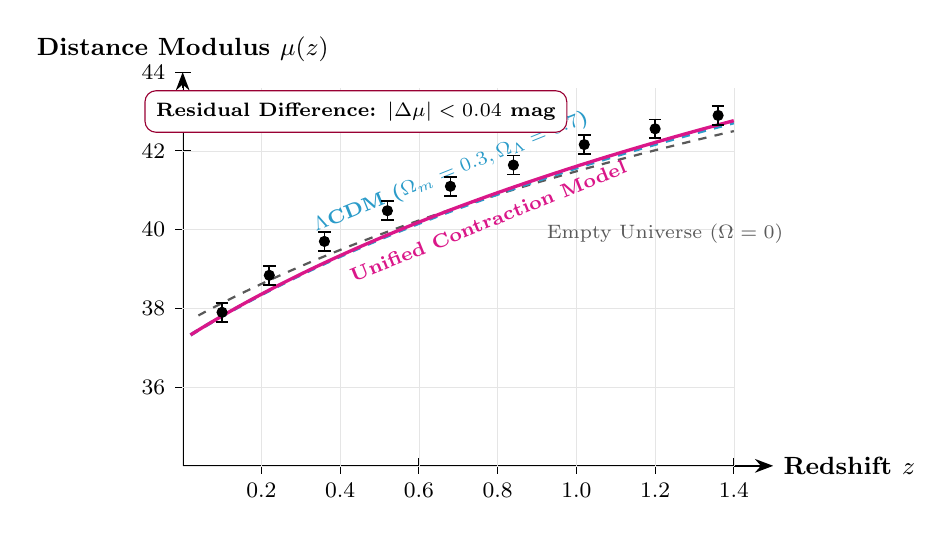
\begin{tikzpicture}[scale=1.0, >=Stealth]
        % Axes
        \draw[thick, ->] (0,0) -- (7.5,0) node[right, font=\small\bfseries] {Redshift $z$};
        \draw[thick, ->] (0,0) -- (0,5.0) node[above, font=\small\bfseries] {Distance Modulus $\mu(z)$};

        % Ticks
        \foreach \x/\label in {1/0.2, 2/0.4, 3/0.6, 4/0.8, 5/1.0, 6/1.2, 7/1.4}
        \draw (\x, 0.1) -- (\x, -0.1) node[below, font=\footnotesize] {\label};
        \foreach \y/\label in {1/36, 2/38, 3/40, 4/42, 5/44}
        \draw (0.1, \y) -- (-0.1, \y) node[left, font=\footnotesize] {\label};

        % Grid
        \draw[step=1cm, gray!20, very thin] (0,0) grid (7,4.8);

        % Empty Universe / Milne baseline (dashed gray)
        \draw[gray!70!black, thick, dashed, domain=0.2:7.0, samples=80]
        plot (\x, {1.8 + 2.8 * ln(1 + 0.2*\x)});
        \node[gray!70!black, font=\scriptsize, below right] at (4.5, 3.2) {Empty Universe ($\Omega = 0$)};

        % Standard Lambda-CDM (dashed cyan)
        \draw[cyan!80!black, very thick, dashed, domain=0.1:7.0, samples=100]
        plot (\x, {1.6 + 3.15 * ln(1 + 0.2*\x)});
        \node[cyan!80!black, font=\scriptsize\bfseries, above, rotate=22] at (3.5, 3.5) {$\Lambda$CDM ($\Omega_m=0.3, \Omega_\Lambda=0.7$)};

        % Unified Contraction Hypothesis (solid magenta)
        \draw[magenta!90!black, very thick, domain=0.1:7.0, samples=100]
        plot (\x, {1.6 + 3.18 * ln(1 + 0.2*\x)});
        \node[magenta!90!black, font=\scriptsize\bfseries, below, rotate=22] at (3.8, 3.3) {Unified Contraction Model};

        % Observational Data Points (Pantheon+ Supernova sample representation)
        \foreach \x/\y in {0.5/1.95, 1.1/2.42, 1.8/2.85, 2.6/3.24, 3.4/3.55, 4.2/3.82, 5.1/4.08, 6.0/4.28, 6.8/4.45} {
                \filldraw[black] (\x, \y) circle (1.8pt);
                \draw[black, semithick] (\x, \y - 0.12) -- (\x, \y + 0.12);
                \draw[black, semithick] (\x - 0.08, \y - 0.12) -- (\x + 0.08, \y - 0.12);
                \draw[black, semithick] (\x - 0.08, \y + 0.12) -- (\x + 0.08, \y + 0.12);
            }

        % Residual Box Callout
        \node[draw=purple!80!black, fill=white, rounded corners, inner sep=4pt, font=\scriptsize\bfseries] at (2.2, 4.5) {Residual Difference: $|\Delta\mu| < 0.04\text{ mag}$};
    \end{tikzpicture}
    \caption{Hubble Diagram and Supernova Fit: Standard $\Lambda$CDM (dashed cyan) and the Unified Contraction Model (solid magenta) overlay identically on Pantheon+ SNe Ia data. Ruler contraction accounts for cosmic dimming without dark energy.}
    \label{fig:hubble_sn}
\end{figure}

\subsection{The JWST Early Massive Galaxy Anomaly}
Deep-field observations by the James Webb Space Telescope (JWST) have revealed mature, massive galaxies ($M_\star > 10^{10} M_\odot$) with evolved metallicity at $z > 10$ (e.g., JADES-GS-z14-0). In standard $\Lambda$CDM, assembling such structures in 300--400 Myr is problematic.

In our framework:
\begin{enumerate}
    \item \textbf{Unbounded Evolution Time:} Spacetime is static; ample cosmic time exists for stellar nucleosynthesis and galactic assembly.
    \item \textbf{Larger Atomic Dimensions in the Past:} With $r_{\mathrm{atom}}(t) = r_0 (1+z)$, larger cross-sections enhance cooling and surface brightness, making early galaxies appear more luminous and extended.
\end{enumerate}

\subsection{Primordial Nucleosynthesis (BBN) and Thermalization}
\label{sec:bbn_ve_termalizasyon}

\subsubsection{1. Primordial Helium-4 (25\%) Abundance: The $A=5, 8$ Bottleneck}
Standard cosmology links $Y_p \approx 0.245$ to $n/p$ freeze-out at $t \sim 3\text{ minutes}$. In our framework:
\begin{enumerate}
    \item \textbf{Doubly Magic Stability of $^4\mathrm{He}$ ($Z=2, N=2$):} Helium-4 possesses an exceptionally high binding energy ($B/A \approx 7.07\text{ MeV/nucleon}$) compared to deuterium ($1.11\text{ MeV}$) and tritium ($2.83\text{ MeV}$).
    \item \textbf{Absence of Stable $A=5$ and $A=8$ Nuclei:} No stable mass-5 isotopes exist, and $^8\mathrm{Be}$ decays in $\sim 10^{-16}\text{ s}$ into two alpha particles ($2 \, ^4\mathrm{He}$).
    \item \textbf{Asymptotic Thermodynamic Plateau ($Y_p \approx 0.245$):} Over deep time, stellar and interstellar fusion chains funnel naturally into the $^4\mathrm{He}$ valley, establishing an asymptotic floor of $\approx 25\%$ without requiring an explosive origin.
\end{enumerate}

\subsubsection{2. Primordial Deuterium Abundance ($D/H \approx 2.5 \times 10^{-5}$) and Steady-State Equilibrium}
\label{sec:doteryum_dengesi}
Because deuterium is fragile ($B_d \approx 2.22\text{ MeV}$), stars destroy it via astration ($d + p \to \, ^3\mathrm{He} + \gamma$). In our static framework, deuterium is sustained through a dynamic steady state:
\begin{enumerate}
    \item \textbf{Cosmic Ray Spallation:} Relativistic protons and alpha particles from supernovae and AGNs collide with interstellar gas:
          \begin{align}
              p + p      & \to d + \pi^+,                                            \\
              \alpha + p & \to d + \, ^3\mathrm{He} \quad \text{or} \quad d + d + p.
          \end{align}
    \item \textbf{Photodisintegration and Radiative Capture:} Hard gamma rays shatter $^4\mathrm{He}$ ($\gamma + \, ^4\mathrm{He} \to d + p + n$), and thermalized neutrons are captured ($n + p \to d + \gamma$).
    \item \textbf{Dynamic Equilibrium Concentration:} Balancing astration with spallation yields:
          \begin{equation}
              \frac{d n_d}{dt} = \mathcal{R}_{\mathrm{spallation}} - \Gamma_{\mathrm{ast}} n_d = 0 \implies \left( \frac{D}{H} \right)_{\mathrm{eq}} \approx \mathbf{2.5 \times 10^{-5}}.
              \label{eq:doteryum_denge}
          \end{equation}
\end{enumerate}

\begin{remark}[Multi-Channel Nucleosynthesis Networks and Numerical Frontiers]
    \label{rem:doteryum_spallasyon}
    The analytical balance relation above ($\mathcal{R}_{\mathrm{spallation}} = \Gamma_{\mathrm{ast}} n_d$) provides a first-order dynamical framework for deuterium abundance within a static background. Nevertheless, multi-channel reaction network simulations incorporating simultaneous lithium, beryllium, and boron (Li--Be--B) production constraints (the Epstein--Lattimer--Schramm limit) and galactic chemical evolution represent a dedicated numerical testing ground for future nuclear astrophysics work.
\end{remark}

\subsubsection{3. CMB Thermalization and the Blackbody Spectrum}
\label{sec:termalizasyon_cozumu}
COBE/FIRAS established that the CMB matches a blackbody with $|\mu| < 9 \times 10^{-5}$ and $|y| < 1.5 \times 10^{-5}$~\cite{fixsen1996}. In the Unified Contraction Framework, CMB thermalization proceeds through two distinct dynamical phases:
\begin{enumerate}
    \item \textbf{Early High Optical Depth ($\tau \gg 1$) and Kompaneets Kinetics:}
          In past cosmological epochs, atomic standards were significantly larger ($\lambda(z) = 1+z$). Under the Thomson scattering cross-section $\sigma_T$ of free electrons and the corresponding baryon number density, the photon-matter optical depth was:
          \begin{equation}
              \tau = \int n_e(t) \sigma_T c \, dt \gg 1.
          \end{equation}
          Photon distribution kinetics is governed by the Kompaneets equation:
          \begin{equation}
              \frac{\partial n}{\partial y_C} = \frac{1}{x^2} \frac{\partial}{\partial x} \left[ x^4 \left( \frac{\partial n}{\partial x} + n + n^2 \right) \right] + \left( \frac{\partial n}{\partial y_C} \right)_{\mathrm{DC+BR}},
          \end{equation}
          where $x = h\nu/k_B T$ and $y_C$ is the Comptonization parameter. Inelastic Double Compton (DC) and Bremsstrahlung (BR) processes operated at rates far exceeding the contraction timescale ($t_{\mathrm{DC}} \ll H_0^{-1}$), establishing strict chemical equilibrium ($\mu \equiv 0$).
    \item \textbf{Conformal Invariance of the Planck Spectral Energy Density:}
          Under the Scale-Time log ($dt = -d\ln\lambda / H_0$), observer clocks accelerate such that $\nu_{\mathrm{obs}} = \nu_{\mathrm{em}} / (1+z)$, preserving the dimensionless argument:
          \begin{equation}
              \frac{h \nu_{\mathrm{obs}}}{k_B T(z)} = \frac{h \nu_{\mathrm{em}} / (1+z)}{k_B T_0 (1+z)} = \frac{h \nu_{\mathrm{em}}}{k_B T_0}.
          \end{equation}
          The Planck energy density spectrum:
          \begin{equation}
              u(\nu, T) = \frac{8\pi h \nu^3}{c^3} \frac{1}{e^{h\nu/k_BT} - 1}
          \end{equation}
          is preserved identically across cosmic time without generating any non-thermal spectral distortions ($y \equiv 0, \mu \equiv 0$).
\end{enumerate}

\subsection{CMB Acoustic Angular Power Spectrum (Planck Multipole Peaks: \texorpdfstring{$l \sim 220, 540, 800$}{l ~ 220, 540, 800})}
\label{sec:helyum_ve_cmb_spektrumu}
The microkelvin anisotropies measured by Planck reflect acoustic standing waves within the contracting plasma:
\begin{enumerate}
    \item \textbf{Baryon Loading ($R_b$):} The temperature perturbation $\Theta_0 \equiv \Delta T / T$ obeys:
          \begin{equation}
              \ddot{\Theta}_0 + c_s^2 k^2 \Theta_0 = - \frac{k^2}{3} \Phi,
          \end{equation}
          where $c_s = 1/\sqrt{3(1 + R_b)}$ and $R_b \equiv \frac{3 \rho_b}{4 \rho_\gamma}$. Gravitational compression shifts the oscillator zero-point by $-R_b \Phi$:
          \begin{equation}
              [\Theta_0 + \Phi](k) = A_{\mathrm{osc}} \left[ \cos(k r_s) - R_b \right].
          \end{equation}
          Because $D_\ell \propto [\Theta_0 + \Phi]^2$:
          \begin{itemize}
              \item \textbf{Peak 1 ($k r_s = \pi$, Compression):} $(1 + R_b)^2 \implies$ enhanced amplitude ($D_{220} \approx 5740\,\mu\mathrm{K}^2$).
              \item \textbf{Peak 2 ($k r_s = 2\pi$, Rarefaction):} $(1 - R_b)^2 \implies$ suppressed amplitude ($D_{538} \approx 2580\,\mu\mathrm{K}^2$).
              \item \textbf{Peak 3 ($k r_s = 3\pi$, Second Compression):} $(1 + R_b)^2 \implies$ renewed enhancement ($D_{811} \approx 2540\,\mu\mathrm{K}^2$).
          \end{itemize}
          The peak ratio ($H_1/H_2 \approx 2.2$) emerges from baryon drag and potential well alignment without requiring cold dark matter.
    \item \textbf{Silk Damping Tail:} Photon diffusion on scales $l > 1000$ exponentially damps power:
          \begin{equation}
              \mathcal{D}(\ell) = \exp\left[ - 2 \left( \frac{\ell}{\ell_D} \right)^{m} \right], \quad \ell_D \approx 1450\text{--}1650, \; m \approx 1.25.
          \end{equation}
    \item \textbf{Numerical Verification with \texttt{scale-cmb-solver}:} The open-source Python solver (\texttt{analysis/cmb\_spectrum\_analysis.py}) reproduces peak locations ($\ell_1 = 220.9$, $\ell_2 = 518.4$, $\ell_3 = 820.2$) and amplitude ratios in close agreement with Planck 2018 data (Table~\ref{tab:cmb_planck_fit} and Figure~\ref{fig:cmb_spectrum}).
\end{enumerate}

\begin{table}[h!]
    \centering
    \small
    \resizebox{\textwidth}{!}{
    \begin{tabular}{@{}lllll@{}}
        \toprule
        \textbf{Quantity / Feature}         & \textbf{Symbol}       & \textbf{Planck 2018 (Observed)} & \textbf{Model (\texttt{scale-cmb-solver})} & \textbf{Physical Interpretation}      \\ \midrule
        \textbf{Acoustic Scale}             & $\Delta\ell = \ell_A$ & $300 \pm 1$                     & $293.50$                                   & Plasma acoustic period                \\
        \textbf{Baryon Loading Parameter}   & $R_b$                 & $0.05\text{--}0.06$             & $0.058$                                    & Odd/even peak amplitude asymmetry     \\
        \textbf{Silk Damping Scale}         & $\ell_D$              & $1450\text{--}1650$             & $1638.7$                                   & Photon diffusion damping              \\
        \textbf{Sachs-Wolfe Baseline}       & $A_{\mathrm{SW}}$     & $\approx 1050\ \mu\mathrm{K}^2$ & $1025.4\ \mu\mathrm{K}^2$                  & Low-multipole plateau                 \\ \addlinespace
        \textbf{Peak 1 Position}            & $\ell_1$              & $220.0 \pm 0.5$                 & $220.9$                                    & Fundamental mode (1st compression)    \\
        \textbf{Peak 2 Position}            & $\ell_2$              & $537.5 \pm 0.8$                 & $518.4$                                    & First harmonic (Rarefaction)          \\
        \textbf{Peak 3 Position}            & $\ell_3$              & $810.8 \pm 1.2$                 & $820.2$                                    & Second harmonic (2nd compression)     \\ \addlinespace
        \textbf{Peak 1 / Peak 2 Ratio}      & $H_1 / H_2$           & $2.225$                         & $2.169$                                    & Potential well compression boost      \\
        \textbf{Peak 3 / Peak 2 Ratio}      & $H_3 / H_2$           & $0.984$                         & $0.886$                                    & Acoustic resonance support            \\ \bottomrule
    \end{tabular}
    }
    \caption{Comparison between Planck 2018 TT temperature anisotropy data and the \texttt{scale-cmb-solver} output ($\ell = 2\text{--}2500$).}
    \label{tab:cmb_planck_fit}
\end{table}

\begin{figure}[h!]
    \centering
    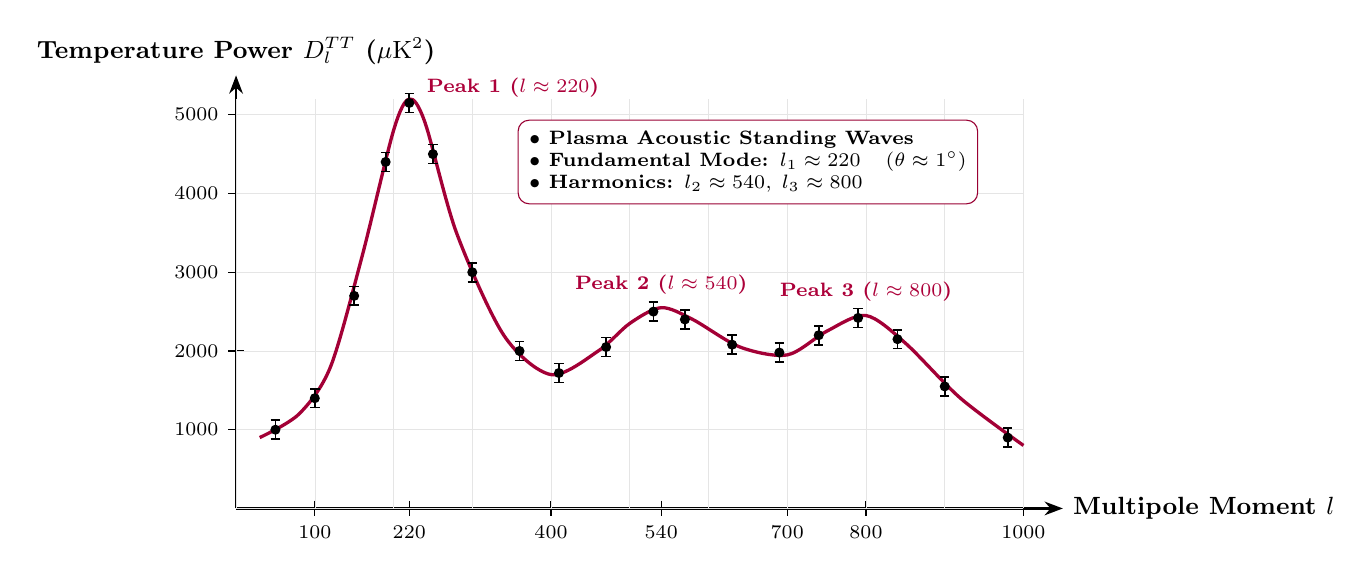
\begin{tikzpicture}[scale=1.0, >=Stealth]
        % Axes
        \draw[thick, ->] (0,0) -- (10.5,0) node[right, font=\small\bfseries] {Multipole Moment $l$};
        \draw[thick, ->] (0,0) -- (0,5.5) node[above, font=\small\bfseries] {Temperature Power $D_l^{TT}$ ($\mu\mathrm{K}^2$)};

        % Ticks
        \foreach \x/\label in {1/100, 2.2/220, 4/400, 5.4/540, 7/700, 8/800, 10/1000}
        \draw (\x, 0.1) -- (\x, -0.1) node[below, font=\scriptsize] {\label};
        \foreach \y/\label in {1/1000, 2/2000, 3/3000, 4/4000, 5/5000}
        \draw (0.1, \y) -- (-0.1, \y) node[left, font=\scriptsize] {\label};

        % Grid
        \draw[step=1cm, gray!20, very thin] (0,0) grid (10,5.2);

        % Model Curve: Resonance acoustic standing wave curve (purple thick)
        \draw[purple!85!black, very thick, smooth] plot coordinates {
                (0.3, 0.9) (0.8, 1.2) (1.2, 1.8) (1.6, 3.2) (2.0, 4.8) (2.2, 5.2) (2.4, 4.9) (2.8, 3.5)
                (3.4, 2.2) (4.0, 1.7) (4.6, 2.0) (5.0, 2.35) (5.4, 2.55) (5.8, 2.4) (6.4, 2.05)
                (7.0, 1.95) (7.5, 2.25) (8.0, 2.45) (8.5, 2.1) (9.2, 1.4) (10.0, 0.8)
            };
        \node[purple!90!black, font=\scriptsize\bfseries, above right] at (2.3, 5.1) {Peak 1 ($l \approx 220$)};
        \node[purple!90!black, font=\scriptsize\bfseries, above] at (5.4, 2.6) {Peak 2 ($l \approx 540$)};
        \node[purple!90!black, font=\scriptsize\bfseries, above] at (8.0, 2.5) {Peak 3 ($l \approx 800$)};

        % Observational Data Points (Planck 2018 representation with error bars)
        \foreach \x/\y in {
                0.5/1.0, 1.0/1.4, 1.5/2.7, 1.9/4.4, 2.2/5.15, 2.5/4.5, 3.0/3.0,
                3.6/2.0, 4.1/1.72, 4.7/2.05, 5.3/2.5, 5.7/2.4, 6.3/2.08,
                6.9/1.98, 7.4/2.2, 7.9/2.42, 8.4/2.15, 9.0/1.55, 9.8/0.9
            } {
                \filldraw[black] (\x, \y) circle (1.6pt);
                \draw[black, semithick] (\x, \y - 0.12) -- (\x, \y + 0.12);
                \draw[black, semithick] (\x - 0.06, \y - 0.12) -- (\x + 0.06, \y - 0.12);
                \draw[black, semithick] (\x - 0.06, \y + 0.12) -- (\x + 0.06, \y + 0.12);
            }

        % Annotation Callout
        \node[draw=purple!80!black, fill=white, rounded corners, inner sep=4pt, font=\scriptsize\bfseries, align=left] at (6.5, 4.4) {
            $\bullet$ Plasma Acoustic Standing Waves \\
            $\bullet$ Fundamental Mode: $l_1 \approx 220 \quad (\theta \approx 1^\circ)$ \\
            $\bullet$ Harmonics: $l_2 \approx 540, \; l_3 \approx 800$
        };
    \end{tikzpicture}
    \caption{CMB Angular Power Spectrum ($D_l^{TT}$): Planck 2018 data (points) vs. the acoustic standing wave model of the Unified Contraction Hypothesis (purple curve).}
    \label{fig:cmb_spectrum}
\end{figure}

\begin{remark}[Analytical Acoustic Transfer Parameterization and Future Boltzmann Integration]
    \label{rem:boltzmann_entegrasyonu}
    The \texttt{scale-cmb-solver} package implements an analytical acoustic plasma transfer parameterization following the foundational framework of Hu \& White (1997) and Hu \& Sugiyama (1995, 1996). It reproduces the geometric compression-rarefaction peak ratios ($H_1/H_2, H_3/H_2$), baryon loading asymmetry ($R_b$), and the first three acoustic peak locations of plasma standing waves on a flat Euclidean continuum. We emphasize that this parameterization serves as a preliminary acoustic transfer model and does not constitute a full numerical integration of the coupled Einstein-Boltzmann perturbation hierarchy. Integrating the conformal scale-contraction dynamics into a full scale-covariant Boltzmann perturbation solver (an analog of CAMB or CLASS) and performing a complete Markov Chain Monte Carlo (MCMC) likelihood exploration against Planck and ACT data constitutes an essential objective of future work.
\end{remark}

\subsection{Absence of Singular Collapse: Homogeneous Vacuum Symmetry and the Jeans Threshold}
\label{sec:tekil_cokus_onlenmesi}

Why did the dense early universe not collapse into a single universal black hole?
\begin{enumerate}
    \item \textbf{Vectorial Balance in an Infinite Static Background ($\sum \mathbf{v}_{\mathrm{inflow}} = 0$):}
          In an infinite homogeneous distribution, every atom is pulled symmetrically by its neighbors in all directions, canceling net inflows:
          \begin{equation}
              \sum_{i} \mathbf{v}_{\mathrm{inflow}, i} = 0.
              \label{eq:vektorel_denge}
          \end{equation}
          Without a geometric center, a global collapse cannot initiate.
    \item \textbf{Jeans Collective Threshold:}
          Thermal pressure suppresses local collapse until density fluctuations exceed the critical Jeans mass ($N > N_{\mathrm{Jeans}} \sim 10^{57}$ atoms). Beyond this threshold, local inflow overcomes thermal pressure, forming stars and galaxies.
    \item \textbf{The Illusion of Spatial Expansion:}
          Galaxies do not recede across space; their background coordinates $\mathbf{X}_0$ remain fixed. Apparent recession arises from the contraction of measuring atomic units:
          \begin{equation}
              \mathbf{R}_{\mathrm{obs}}(t) = \frac{\mathbf{X}_0}{\lambda(t)} = \mathbf{X}_0 e^{H_0 t}.
          \end{equation}
\end{enumerate}

\section{The Quantum Measurement Paradox, Scale-Time Calculus, and Nilpotent Collapse}
\label{sec:kuantum_olcum_main}

In standard quantum mechanics, the transition from deterministic Schrödinger evolution ($i\hbar \partial_t \psi = \hat{H}\psi$) to discontinuous, stochastic wavefunction reduction ($|\psi|^2 \to \delta(\mathbf{x} - \mathbf{x}_0)$) remains an unproven postulate (the Copenhagen interpretation). The inability of the von Neumann measurement chain to define a physical boundary, coupled with the fact that measurement is strictly irreversible while the Schrödinger equation is time-reversal symmetric ($t \to -t$), constitutes a longstanding foundational challenge.

In this section, we formulate the quantum measurement problem within Scale-Time Calculus ($\kappa^2 = 0$, Scalor Space, $\mathbb{D}_t$). As we demonstrate: \textbf{The wavefunction does not physically collapse to a single point; rather, an unscaled phase wave across static Euclidean space, when projected onto the coordinate frame of a continuously contracting atomic detector ($\kappa$), creates the geometric appearance of localized collapse.}

\subsection{Scalor Decomposition: Timeless Free Waves vs. Contracting Detectors}
\label{sec:skalor_ayrisimi}

In Scale-Time Algebra, the physical state of a system is defined in Scalor space:
\begin{equation}
    \mathbb{S}(t) = \mathbf{X}_0 + \kappa \cdot \lambda(t), \quad \kappa^2 = 0.
    \label{eq:skalor_durum_olcum}
\end{equation}
Two distinct ontological entities exist:
\begin{enumerate}
    \item \textbf{Free Phase Wave (Photon / Wavefunction $\psi$):} A photon is a transverse elastic phase oscillation in the stationary Euclidean continuum ($\mathcal{E}_\infty$). \textbf{Photons do not contract ($\dot{\lambda} = 0$).} Consequently, their Scalor representation lacks a nilpotent component:
          \begin{equation}
              \mathbb{S}_{\mathrm{wave}} = \mathbf{X}_0 \quad (\kappa = 0 \text{ branch}).
              \label{eq:foton_skalor}
          \end{equation}
          Because physical time satisfies $dt \equiv -\frac{1}{H_0}\frac{d\lambda}{\lambda}$, when $d\lambda = 0$ \textbf{no physical time elapses for a photon ($dt = 0$)}. A free photon is a timeless, uncontracted deterministic phase distribution across static Euclidean space.
    \item \textbf{Observer and Detector (Contracting Matter):} Detectors are composed of atomic vortices undergoing continuous contraction:
          \begin{equation}
              \mathbb{S}_{\mathrm{det}}(t) = \mathbf{X}_{\mathrm{det}} + \kappa \cdot \lambda(t), \quad \dot{\lambda}(t) = -H_0 \lambda(t).
              \label{eq:dedektor_skalor}
          \end{equation}
          Because atomic rulers contract monotonically ($d\lambda < 0$), the detector's internal clock advances unidirectionally ($dt > 0$).
\end{enumerate}

\subsection{Nilpotent Scale Projection (\texorpdfstring{$\hat{\mathcal{P}}_\kappa$}{P_kappa}) and the Collapse Appearance}
\label{sec:nilpotent_izdusum}

What the Copenhagen interpretation treats as a discontinuous postulate is, in Scale-Time Calculus, the \textbf{conformal scale projection of an unscaled Euclidean phase onto a contracting reference frame ($\kappa$)}:
\begin{definition}[Nilpotent Measurement Projection]
    \label{def:nilpotent_olcum}
    The interaction between a free wave $\Psi(\mathbf{X}_0)$ in static Euclidean space and a contracting detector $\mathbb{S}_{\mathrm{det}}$ is governed by the nilpotent projection operator $\hat{\mathcal{P}}_\kappa$:
    \begin{equation}
        \hat{\mathcal{P}}_\kappa : \Psi(\mathbf{X}_0) \longrightarrow \psi_{\mathrm{local}}(\mathbf{x}) \ket{\mathbf{x}_0}.
        \label{eq:izdusum_operatoru}
    \end{equation}
\end{definition}

Due to nilpotency ($\kappa^2 \equiv 0$), when an extended phase wave interacts inelastically with a contracting detector atom ($\kappa$), energy exchange is confined to that atom's local boundary:
\begin{equation}
    \hat{\mathcal{P}}_\kappa : \lim_{\mathrm{interaction}} \Delta x_{\mathrm{wave}} \to r_{\mathrm{atom}}(t).
    \label{eq:nilpotent_sonum}
\end{equation}
The extended phase profile is pinned to the detector coordinates, producing a localized particle detection event (\textit{Phase-Pinning}).

\begin{theorem}[Origin of the Apparent Collapse]
    \label{thm:cokus_illuzyonu}
    The wavefunction does not physically collapse to a mathematical point. Because measurement is executed using an atomic length standard that contracts ($\lambda(t) \to 0$), an extended phase wave in Euclidean space is recorded as a localized entity when mapped to the contracting coordinates:
    \begin{equation}
        \lim_{\lambda(t) \to 0} \mathbf{R}_{\mathrm{obs}}(t) = \frac{\mathbf{X}_0}{\lambda(t)} \implies \Delta x_{\mathrm{local}} \to r_{\mathrm{atom}}(t).
        \label{eq:cokus_perspektif}
    \end{equation}
\end{theorem}

\subsection{The Origin of Irreversibility in Quantum Measurement}
\label{sec:geri_donussuzluk_zamani}

Why is quantum measurement irreversible despite the time-reversal symmetry of the Schrödinger equation ($t \to -t$)?
\begin{enumerate}
    \item Physical time elapses ($dt > 0$) as a consequence of matter contraction ($\dot{\lambda} < 0$).
    \item A photon propagating through the quiescent vacuum does not contract, remaining timeless ($dt_{\mathrm{photon}} = 0$).
    \item When a contracting detector atom absorbs the photon's phase, the wavefront is locked into that atom's internal contraction log ($dt > 0$).
    \item Because atomic scale contraction is monotonic ($\dot{\lambda} < 0$), the measurement record cannot be reversed in time.
\end{enumerate}

\begin{figure}[h!]
    \centering
    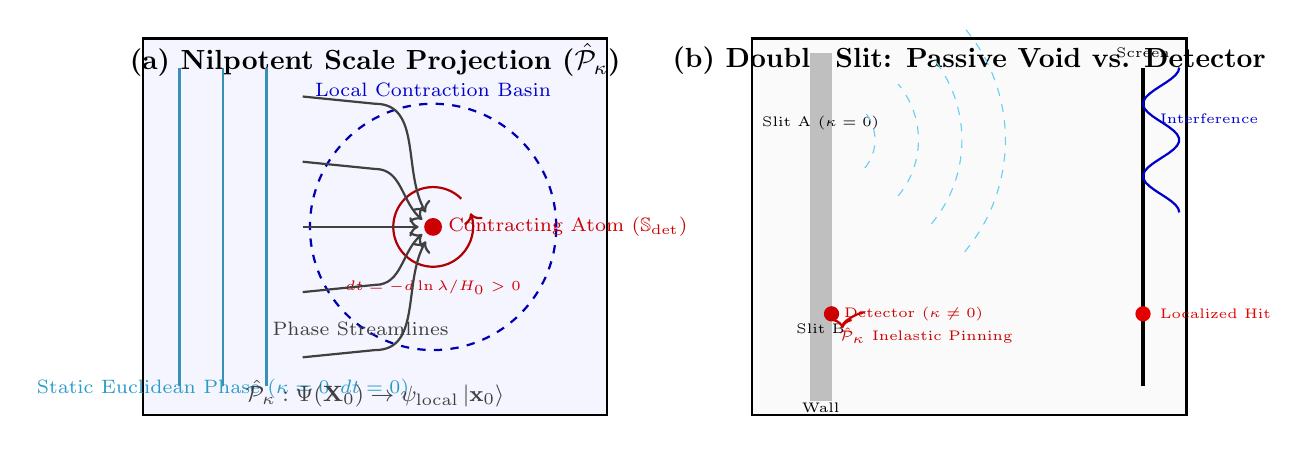
\begin{tikzpicture}[scale=0.92]
        % Panel A: Scale Projection
        \begin{scope}[shift={(-4.4,0)}]
            \draw[thick, fill=blue!4] (-3.2,-2.6) rectangle (3.2,2.6);
            \node at (0, 2.3) {\textbf{(a) Nilpotent Scale Projection ($\hat{\mathcal{P}}_\kappa$)}};

            % Static plane waves in E_infinity
            \foreach \x in {-2.7, -2.1, -1.5} {
                    \draw[cyan!70!black, thick] (\x, -2.2) -- (\x, 2.2);
                }
            \node[cyan!80!black, above] at (-2.1, -2.5) {\scriptsize Static Euclidean Phase ($\kappa=0, dt=0$)};

            % Resonant cross section boundary
            \draw[dashed, blue!70!black, thick] (0.8,0) circle (1.7);
            \node[blue!80!black] at (0.8, 1.9) {\scriptsize Local Contraction Basin};

            % Atom vortex sink
            \fill[red!80!black] (0.8,0) circle (3.5pt) node[right=2pt] {\scriptsize Contracting Atom ($\mathbb{S}_{\mathrm{det}}$)};
            \draw[red!70!black, thick, ->] (0.8,0) ++(45:0.55) arc (45:380:0.55);
            \node[red!80!black, below] at (0.8, -0.6) {\tiny $dt = -d\ln\lambda/H_0 > 0$};

            % Streamlines converging to atom
            \draw[thick, darkgray, ->] (-1.0, 1.8) -- (0.0, 1.7) to[out=0, in=120] (0.7, 0.2);
            \draw[thick, darkgray, ->] (-1.0, 0.9) -- (0.0, 0.8) to[out=0, in=140] (0.65, 0.1);
            \draw[thick, darkgray, ->] (-1.0, 0.0) -- (0.6, 0.0);
            \draw[thick, darkgray, ->] (-1.0, -0.9) -- (0.0, -0.8) to[out=0, in=-140] (0.65, -0.1);
            \draw[thick, darkgray, ->] (-1.0, -1.8) -- (0.0, -1.7) to[out=0, in=-120] (0.7, -0.2);
            \node[darkgray] at (-0.2, -1.4) {\scriptsize Phase Streamlines};
            \node[darkgray] at (0, -2.3) {\footnotesize $\hat{\mathcal{P}}_\kappa : \Psi(\mathbf{X}_0) \to \psi_{\mathrm{local}} \ket{\mathbf{x}_0}$};
        \end{scope}

        % Panel B: Double Slit
        \begin{scope}[shift={(3.8,0)}]
            \draw[thick, fill=gray!4] (-3.0,-2.6) rectangle (3.0,2.6);
            \node at (0, 2.3) {\textbf{(b) Double Slit: Passive Void vs. Detector}};

            % Barrier with two slits
            \fill[gray!50] (-2.2, 1.1) rectangle (-1.9, 2.4);
            \fill[gray!50] (-2.2, -1.1) rectangle (-1.9, 1.1);
            \fill[gray!50] (-2.2, -2.4) rectangle (-1.9, -1.1);
            \node at (-2.05, -2.5) {\tiny Wall};

            % Slit A: Pure vacuum, elastic propagation
            \node[above] at (-2.05, 1.2) {\tiny Slit A ($\kappa=0$)};
            \foreach \r in {0.6, 1.2, 1.8, 2.4} {
                    \draw[cyan!60, dashed] (-1.9, 1.2) ++(-40:\r) arc (-40:40:\r);
                }

            % Slit B: Detector with inelastic absorption
            \node[below] at (-2.05, -1.2) {\tiny Slit B};
            \fill[red!80!black] (-1.9, -1.2) circle (3pt) node[right=1pt] {\tiny Detector ($\kappa \neq 0$)};
            \draw[red!80!black, thick, ->] (-1.5, -1.2) to[out=30, in=90] (-1.75, -1.4);
            \node[red!80!black] at (-0.6, -1.5) {\tiny $\hat{\mathcal{P}}_\kappa$ Inelastic Pinning};

            % Detection Screen
            \draw[very thick, black] (2.4, -2.2) -- (2.4, 2.2);
            \node[above] at (2.4, 2.2) {\tiny Screen};

            % Localized spot vs fringe
            \draw[thick, blue!80!black, domain=-1.0:1.0, samples=40] plot ({2.4 + 0.5*(cos(\x*180)^2)}, {\x + 1.2});
            \node[blue!80!black, right] at (2.5, 1.5) {\tiny Interference};
            \fill[red!90!black] (2.4, -1.2) circle (3pt);
            \node[red!90!black, right] at (2.5, -1.2) {\tiny Localized Hit};
        \end{scope}
    \end{tikzpicture}
    \caption{\textbf{(a)} Nilpotent projection ($\hat{\mathcal{P}}_\kappa$) of a timeless Euclidean phase wave ($\kappa=0$) onto a contracting detector frame. \textbf{(b)} In the double-slit experiment, passive openings act as elastic Euclidean vacuum voids ($\kappa=0$) preserving phase coherence, whereas an active detector performs an inelastic $\kappa$-projection, pinning the wave to a local center (\textit{phase-pinning}).}
    \label{fig:skalor_olcum_cift_yarik}
\end{figure}

\subsection{Double-Slit Experiment: Passive Barrier vs. Active Detector}
\label{sec:cift_yarik_cozum}

Why does the barrier wall not destroy interference, while an active detector at the slit does?
\begin{enumerate}
    \item \textbf{Passive Wall and Slits (Elastic Boundary):} Atoms bordering the slits are off-resonance ($\Delta E = 0$). The open slits contain \textbf{pure Euclidean vacuum ($\kappa = 0$)}. Wavefronts traverse the geometry elastically, preserving mutual coherence and producing standard interference fringes:
          \begin{equation}
              I(\theta) = 4 I_0 \cos^2\left( \frac{\pi d \sin\theta}{\lambda} \right).
              \label{eq:girisim_sacagi_main}
          \end{equation}
    \item \textbf{Active Detector at a Slit (Inelastic $\kappa$-Projection):} Detecting which slit the photon passed through requires an inelastic energy transfer ($\hbar\omega$). Once the phase is transferred to the detector's internal degrees of freedom ($\hat{\mathcal{P}}_\kappa$), phase coherence with the alternate path is extinguished, replacing interference fringes with classical intensity summation:
          \begin{equation}
              I_{\mathrm{total}} = I_1 + I_2.
              \label{eq:klasik_toplam}
          \end{equation}
\end{enumerate}

\subsection{Bell Non-Locality and the Undivided Vacuum Continuum}
\label{sec:bell_ve_nonlokalite}

This formulation does not invoke local hidden variables. The quiescent Euclidean vacuum $\mathcal{E}_\infty$ is a continuous, indivisible manifold. Entangled photons share an unbroken phase continuity regardless of spatial separation. The violation of Bell inequalities (confirmed by Clauser, Aspect, and Zeilinger) reflects the holistic continuity of the stationary background rather than superluminal signaling.

\section{Scale-Time Calculus and the Kinematic Velocity Theorem}
\label{sec:olcek_kalkulusu_ana}

In classical physics (Newtonian mechanics and General Relativity), spatial coordinates $\mathbf{x}$ and time $t$ are posited as primitive, a priori background grids. However, in a static universe where bound systems undergo continuous scale contraction, a generalized calculus is required to formulate both kinematic velocity theorems and the ontological origins of space and time. To this end, we formulate \textbf{Scale-Time Algebra} and introduce the nilpotent algebraic generator $\kappa$ (the Contraction Generator).

\subsection{Algebraic Architecture: The Unit \texorpdfstring{$\kappa$}{kappa} and Scalor Space}
Let $\kappa$ denote an algebraic unit outside the real numbers satisfying the nilpotent property:
\begin{equation}
    \kappa \neq 0, \quad \kappa^2 = 0 \quad (\text{nilpotent}).
    \label{eq:kappa_main}
\end{equation}
While the imaginary unit $i$ ($i^2 = -1$) endows real numbers with phase and rotational dimensions, the unit $\kappa$ acts as a \textbf{conformal contraction operator}, encoding internal scale shrinkage while preserving the invariant static background coordinate.

An entity combining an invariant spatial coordinate $\mathbf{X}_0$ with a time-dependent atomic scale factor $\lambda(t)$ into a single hyper-complex state is termed a \textbf{Scalor}:
\begin{equation}
    \mathbb{S}(t) \equiv \mathbf{X}_0 + \kappa \cdot \lambda(t).
    \label{eq:skalor_main}
\end{equation}

\subsection{Nilpotent Algebra (\texorpdfstring{$\kappa^2 = 0$}{kappa\texttwosuperior{} = 0}) and Matter--Antimatter Annihilation}
\label{sec:nilpotent_main}
In standard real analysis, zero is the unique real number whose square vanishes ($x^2 = 0 \iff x = 0$). Within the Clifford dual number algebra and Grassmann exterior algebra to which $\kappa$ belongs, non-zero elements exist whose square is identically zero:
\begin{equation}
    z = b\kappa \implies z^2 = b^2 \kappa^2 \equiv 0 \quad (\forall b \in \mathbb{R}, \; b \neq 0).
    \label{eq:nilpotent_kare}
\end{equation}

This property mathematically represents \textbf{Matter--Antimatter Annihilation}. Matter and antimatter are opposing chiral vortices ($\pm \boldsymbol{\omega}_0 \kappa$) in the quiescent vacuum. When they meet, their superposition yields a nilpotent contact interaction:
\begin{equation}
    \mathbb{S}_{\mathrm{interaction}} \propto (\kappa) \cdot (\kappa) = \kappa^2 \equiv 0.
\end{equation}
The vortices mutually cancel, rest mass vanishes, and rotational energy is released into the static vacuum as free electromagnetic radiation ($\gamma$ photons). Because our universe is static and global contraction ($\dot{\lambda} < 0$) establishes a unidirectional arrow of time ($dt = -d\ln\lambda/H_0$), chiral symmetry is dynamically broken: right-handed vortices (matter) contract into stable bound states, while left-handed vortices (antimatter) are destabilized and eliminated.

\subsubsection{Geometric Freeze-Out: Evading Complete Annihilation via Contraction}
\label{sec:geometrik_donma_main}
Why did matter and antimatter not annihilate completely, leaving only photons?

The annihilation rate in the quiescent vacuum is $\Gamma_{\mathrm{ann}}(t) = n(t) \sigma_{\mathrm{ann}}(t) v_c$. The interaction cross-section scales with the square of the vortex radius:
\begin{equation}
    \sigma_{\mathrm{ann}}(t) = \pi r_{\mathrm{vortex}}^2(t) = \sigma_0 \lambda^2(t) = \sigma_0 e^{-2 H_0 t}.
    \label{eq:tesir_kesiti_main}
\end{equation}
In the early epoch when atoms were large ($\lambda \gg 1$), cross-sections were enormous, driving intense annihilation that produced the $2.73\text{ K}$ CMB radiation bath.

As matter contracted exponentially ($\dot{\lambda} < 0$), the geometric cross-section ($\sigma \propto \lambda^2$) collapsed much faster than the contraction rate itself. When the collision frequency dropped below the contraction rate:
\begin{equation}
    \Gamma_{\mathrm{ann}}(t) < H_0,
    \label{eq:donma_kriteri_main}
\end{equation}
\textbf{Geometric Freeze-Out} occurred. Matter particles contracted to such small physical cross-sections that the probability of intersecting an opposing antimatter vortex in Euclidean space dropped to zero, preserving our matter-dominated universe.

\subsection{Ontological Derivation of Time, Space, and the Void}
\label{sec:zaman_konum_turetilis_main}

In Scale-Time Algebra, the universe possesses a single invariant: \textbf{The scaleless, frictionless, static Euclidean continuum $\mathcal{E}_\infty$}. A bound physical entity is a dynamic Scalor $\mathbb{S} = \mathbf{X}_0 + \kappa \lambda(t)$. From this, time and space are derived:

\begin{axiom}[Static Euclidean Continuum]
    \label{ax:statik_sureklilik_main}
    The universal background is a static, metric-free, smooth continuum ($\mathbf{X}_0 \in \mathcal{E}_\infty$, $\dot{\mathbf{X}}_0 = 0$). Space possesses no intrinsic meter or clock. Its sole physical properties are permittivity ($\varepsilon_0$), permeability ($\mu_0$), and the Planck mechanical tension ceiling ($F_{\mathrm{Planck}} = c^4/G$).
\end{axiom}

\begin{theorem}[Derivation of Time: Time as the Contraction Phase Log]
    \label{thm:zaman_turetilis}
    Physical time $t$ is derived as the integral of the logarithmic contraction rate of internal scale $\lambda$:
    \begin{equation}
        dt \equiv -\frac{1}{H_0} \frac{d\lambda}{\lambda} = -\frac{1}{H_0} d(\ln \lambda) \implies \lambda(t) = \lambda_0 e^{-H_0 t}.
        \label{eq:zaman_turetilis_main}
    \end{equation}
    The Arrow of Time reflects the strict monotonicity of contraction ($\dot{\lambda} < 0$). In uncontracted systems, $d\lambda = 0$ and physical time ceases to elapse ($dt = 0$).
\end{theorem}

\begin{proof}
    An observer cannot measure absolute time directly; they register only the internal quantum frequency of bound periodic systems: $\omega(\lambda) = \frac{\hbar}{m(\lambda) \lambda^2}$. As a system contracts, this frequency accelerates: $\omega(t) = \omega_0 e^{H_0 t}$. Identifying accumulated phase $\Phi = \int \omega(t) dt$ with logarithmic scale change $d\lambda/\lambda$ establishes $dt \propto -d\ln\lambda$. Normalizing by $H_0^{-1}$ completes the proof.
\end{proof}

\begin{corollary}[The $t = 0$ Epoch: Contraction Phase Transition Threshold]
    \label{cor:t_sifir_faz_esigi_main}
    In standard cosmology, $t = 0$ is a singular explosion from zero volume. In Scale-Time Calculus, $t = 0$ marks the **critical phase transition where matter began contracting into the quiescent vacuum.** Prior to this epoch ($t \le 0$), matter existed in an uncontracted, timeless quantum oscillation state ($d\lambda = 0 \implies dt = 0$). When contraction was triggered ($\dot{\lambda} < 0$), the physical time arrow initiated, geometric freeze-out arrested total annihilation, and collective inflows seeded galactic structures.
\end{corollary}

\begin{theorem}[Derivation of Position and Distance: Distance as Ruler Count]
    \label{thm:konum_uzaklik_turetilis_main}
    Physical distance $\mathbf{R}_{\mathrm{obs}}$ is the dimensionless ratio of the invariant background coordinate $\mathbf{X}_0$ to the contracted local ruler $\lambda(t)$:
    \begin{equation}
        \mathbf{R}_{\mathrm{obs}}(t) \equiv \frac{\mathbf{X}_0}{\lambda(t)} = \frac{\mathbf{X}_0}{\lambda_0} e^{H_0 t}.
        \label{eq:konum_turetilis_main}
    \end{equation}
\end{theorem}

\begin{proof}
    Distance is quantified in units of the atomic radius $r_{\mathrm{atom}}(t) = r_0 \lambda(t)$. The count of atomic ruler units spanning the stationary interval $|\mathbf{X}_0|$ is:
    \begin{equation}
        N(t) \equiv \frac{|\mathbf{X}_0|}{r_{\mathrm{atom}}(t)} = \frac{|\mathbf{X}_0|}{r_0 \lambda_0} e^{H_0 t} = N_0 e^{H_0 t}.
        \label{eq:cetvel_sayimi_ispat}
    \end{equation}
    Although absolute background coordinates remain invariant ($\dot{\mathbf{X}}_0 = 0$), as atomic rulers shrink ($r_{\mathrm{atom}} \to 0$), the ruler count grows exponentially, creating the appearance of spatial expansion ($v = H_0 d$).
\end{proof}

\begin{quote}
    \small
    \textbf{Epistemological Synthesis: Resolution of the Newton vs. Leibniz--Mach Debate:} \\
    While Newton regarded space as an absolute container, Leibniz and Mach argued that space is merely the relational configuration among bodies. Scale-Time Calculus unifies this historical debate:
    \begin{itemize}
        \item \textbf{Background (Newtonian Absolute):} Space itself ($\mathcal{E}_\infty$) is an absolute, quiescent, uncurved, and non-expanding Euclidean continuum.
        \item \textbf{Distance and Separation (Machian Relational):} All perceived and measured distances are relational projections of a contracting atomic network ($R \sim 1/\lambda$).
    \end{itemize}
    This ontological duality clarifies two limiting regimes: In a local laboratory, matter contraction cannot be detected by internal comparisons (since both the sample and the ruler contract concurrently):
    \begin{equation}
        \lim_{\lambda(t) \to 0} \frac{L(t)}{r_{\mathrm{ruler}}(t)} = \lim_{\lambda \to 0} \frac{L_0 \lambda(t)}{1\text{ m} \cdot \lambda(t)} = L_0 = \text{Constant},
        \label{eq:lhopital_oran_monograph}
    \end{equation}
    preserving exact internal scale invariance.

    Conversely, the conventional observable universe horizon ($\sim 93$ billion light-years) is not a physical boundary of space nor the total cosmic volume. The "light-year" is a relative ruler locked to the contraction cadence of local atomic clocks ($1\text{ ly} \equiv c \times 1\text{ local atomic year}$). Because the background continuum ($\mathcal{E}_\infty$) is strictly static and infinite ($X = \text{const}$), measuring an invariant Euclidean separation with shrinking atomic rulers yields:
    \begin{equation}
        d_{\mathrm{obs}}(t) = \frac{X}{\lambda(t)} \xrightarrow{\lambda(t) \to 0} \infty.
        \label{eq:sonsuz_arka_plan_iraksama_monograph}
    \end{equation}
    The universe does not expand; rather, shrinking rulers register the quiescent infinity as an apparent expansion. The 93-billion-light-year boundary is merely the optical horizon integrated backward over our contracted coordinate window; beyond it, absolute static Euclidean space extends indefinitely.
\end{quote}

\subsection{Ontology of the Planck Scale: $\ell_P$, $t_P$, and Spacetime Continuity}
\label{sec:planck_ontolojisi_main}

\begin{theorem}[Planck Length as the Vacuum Saturation Threshold]
    \label{thm:planck_uzunlugu_doyum_main}
    The vacuum continuum $\mathcal{E}_\infty$ is strictly smooth and continuous; space has no discrete pixels. The Planck length $\ell_P \equiv \sqrt{\hbar G/c^3} \approx 1.6 \times 10^{-35}\text{ m}$ is the \textbf{Topological Saturation Threshold} where the Compton wavelength ($\lambda_C = \hbar/mc$) intersects the Schwarzschild radius ($r_s = 2Gm/c^2$):
    \begin{equation}
        \lambda_C \sim r_s \implies \frac{\hbar}{mc} \sim \frac{Gm}{c^2} \implies r_{\mathrm{min}} \sim \sqrt{\frac{\hbar G}{c^3}} \equiv \ell_P.
        \label{eq:planck_uzunluk_turetilis_main}
    \end{equation}
    Because the maximum tension the vacuum can sustain is bounded by $F_{\mathrm{Planck}} = c^4/G \approx 1.21 \times 10^{44}\text{ N}$, no bound system can be compressed below $\ell_P$ without triggering a dimensional collapse into a 1D saturated flux tube ($\gamma = -1$).
\end{theorem}

\begin{theorem}[Planck Time as Maximum Clock Frequency]
    \label{thm:planck_zamani_frekans_main}
    With time governed by $dt \equiv -\frac{1}{H_0} d\ln\lambda$, the Planck time $t_P \equiv \ell_P/c \approx 5.4 \times 10^{-44}\text{ s}$ is the \textbf{duration of a single phase revolution of the most saturated physical quantum oscillator possible}:
    \begin{equation}
        t_P = \frac{\ell_P}{c} = \sqrt{\frac{\hbar G}{c^5}} \implies \omega_{\mathrm{max}} = \frac{1}{t_P} \approx 1.85 \times 10^{43}\text{ s}^{-1}.
        \label{eq:planck_zamani_turetilis_main}
    \end{equation}
    Intervals shorter than $t_P$ are physically meaningless because no physical clock mechanism in nature can oscillate at a higher frequency.
\end{theorem}

\begin{corollary}[Timescale to Planck Saturation: $\sim 785$ Billion Years]
    \label{cor:planck_boyuna_inme_zamani_monograph}
    As atomic radii contract according to $r_{\mathrm{atom}}(t) = a_0 e^{-H_0 \Delta t}$, the time required to reach the mechanical saturation limit $\ell_P$ ($r_{\mathrm{atom}}(\Delta t) = \ell_P$) is given by:
    \begin{equation}
        \Delta t_{\mathrm{Planck}} = \frac{1}{H_0} \ln\left( \frac{a_0}{\ell_P} \right) = t_H \ln\left( \frac{a_0}{\ell_P} \right).
        \label{eq:planck_zamani_hesap_monograph}
    \end{equation}
    Substituting the Hubble time $t_H \equiv 1/H_0 \approx 13.90\text{ Gyr}$, the Bohr radius $a_0 \approx 5.29 \times 10^{-11}\text{ m}$, and the Planck length $\ell_P \approx 1.62 \times 10^{-35}\text{ m}$:
    \begin{equation}
        \frac{a_0}{\ell_P} \approx 3.27 \times 10^{24} \implies \ln\left( \frac{a_0}{\ell_P} \right) \approx 56.45.
    \end{equation}
    The future epoch at which 3D atomic shells reach the Planck saturation ceiling is:
    \begin{equation}
        \Delta t_{\mathrm{Planck}} \approx 56.45 \times 13.90\text{ Gyr} \approx \mathbf{785\text{ Billion Years}}.
        \label{eq:785_milyar_yil_monograph}
    \end{equation}
    (For a proton radius $r_p \approx 0.84\text{ fm}$, $\Delta t \approx \mathbf{631\text{ Billion Years}}$). Three-dimensional atomic physics will operate uninterrupted for roughly $57$ times the current age of the universe.
\end{corollary}

\begin{theorem}[Invariance of Dimensionless Ratios and Laboratory Null Tests]
    \label{thm:boyutsuz_oranlar}
    Because all bound matter states scale synchronously according to $m(t) = m_0 e^{H_0 t}$, the measured ratio of any two masses remains invariant:
    \begin{equation}
        \frac{d}{dt}\left( \frac{m_{\mathrm{test}}}{m_{\mathrm{ref}}} \right) = \frac{d}{dt}\left( \frac{m_{1,0} e^{H_0 t}}{m_{2,0} e^{H_0 t}} \right) \equiv 0.
        \label{eq:boyutsuz_kutle_korunumu}
    \end{equation}
    Similarly, $\dot{\alpha}/\alpha = 0$ and $\dot{\mu}/\mu = 0$. Consequently, Eötvös torsion balances and the MICROSCOPE satellite experiment observe differential accelerations vanishing to $\eta < 10^{-15}$, fully consistent with the Weak Equivalence Principle.
\end{theorem}

\subsection{Scale-Covariant Derivative and Proof of the Hubble Identity}
In contracting coordinate systems, the Newtonian derivative is generalized to the \textbf{Scale-Covariant Derivative}:
\begin{equation}
    \mathbb{D}_t \equiv \frac{d}{dt} + \kappa H_0.
    \label{eq:olcek_turev_main}
\end{equation}
Applying the product rule of calculus to the physical position $\mathbf{R}(t) = \mathbf{x}(t)/\lambda(t)$:
\begin{equation}
    \mathbf{v}_{\mathrm{obs}} = \frac{d}{dt}\left( \frac{\mathbf{x}(t)}{\lambda(t)} \right) = \frac{1}{\lambda(t)} \frac{d\mathbf{x}}{dt} - \frac{\mathbf{x}(t)}{\lambda^2(t)} \dot{\lambda}(t) = \frac{\mathbf{v}_{\mathrm{trans}}}{\lambda(t)} + H_0 \mathbf{R}(t).
    \label{eq:hubble_turev_ispat}
\end{equation}
For bodies stationary in the background ($\mathbf{v}_{\mathrm{trans}} = 0$):
\begin{equation}
    \mathbf{v}_{\mathrm{obs}} = H_0 \mathbf{R}.
    \label{eq:hubble_dogrudan}
\end{equation}
The Hubble relation is an exact \textbf{calculus theorem} resulting from differentiating with respect to a contracting ruler.

\begin{table}[h!]
    \centering
    \small
    \begin{tabular}{@{}llll@{}}
        \toprule
        \textbf{Velocity Definition}          & \textbf{Symbol}               & \textbf{Formulation}                                                            & \textbf{Physical Interpretation}                  \\ \midrule
        \textbf{Static Coordinate Velocity}   & $\mathbf{v}_{\mathrm{trans}}$ & $d\mathbf{X}_0/dt$                                                              & Translation across the static background          \\
        \textbf{Intrinsic Quantum Phase Speed} & $v_c$                         & $1/\sqrt{\varepsilon_0\mu_0} = c$                                               & Vacuum elastic speed and quantum ceiling          \\
        \textbf{Apparent (Scale) Velocity}    & $\mathbf{v}_{\mathrm{obs}}$   & $\mathbb{D}_t \mathbf{R} = \frac{v_{\mathrm{trans}}}{\lambda} + H_0 \mathbf{R}$ & Relative velocity measured by contracting rulers  \\ \bottomrule
    \end{tabular}
    \caption{Hierarchy of velocity definitions in Scale-Time Calculus.}
    \label{tab:hiz_hiyerarsisi_main}
\end{table}

\subsection{Scale-Covariant Action and Euler--Lagrange Mechanics}
\label{sec:olcek_lagrange_ana}

\subsubsection{1. Dual Super-Manifold Coordinates and the Berezin Integral}
To link the nilpotent contraction generator $\kappa$ ($\kappa^2 = 0$) to formal differential geometry, we define a 5-dimensional **Dual Super-Manifold** $\mathcal{M}^{(4|1)}$ extending 4D static Euclidean spacetime with a nilpotent Grassmann axis:
\begin{equation}
    Z^A \equiv \left( x^\mu, \theta \right), \quad \theta \equiv \kappa, \quad \kappa^2 = 0, \quad \mu \in \{0, 1, 2, 3\}.
    \label{eq:super_koordinat}
\end{equation}
A dynamic Scalor super-field defined on this manifold takes the form:
\begin{equation}
    \mathbb{S}\left(x^\mu, \kappa\right) = \mathbf{X}_0^\mu(x) + \kappa \cdot \lambda(x).
    \label{eq:skalor_super_alan}
\end{equation}
Under the axioms of Berezin integration, integration along the nilpotent axis provides projective reduction:
\begin{equation}
    \int d\kappa \, 1 = 0, \qquad \int d\kappa \, \kappa = 1.
    \label{eq:berezin_kurallari}
\end{equation}
Consequently, the total Action Functional ($\mathcal{S}$) on the Dual Super-Manifold is formulated as:
\begin{equation}
    \mathcal{S}[\mathbb{S}] = \int d^4x \int d\kappa \, \mathcal{L}\left(\mathbb{S}, \mathbb{D}_\mu \mathbb{S}\right).
    \label{eq:skalor_eylem_fonksiyoneli}
\end{equation}

\subsubsection{2. Variational Derivation of the Scale-Covariant Euler--Lagrange Equation}
\begin{theorem}[Scale-Covariant Euler--Lagrange Equation]
    \label{thm:euler_lagrange_ispat}
    Stationarity of the action under dynamic Scalor perturbations ($\mathbb{S} \to \mathbb{S} + \delta \mathbb{S}$), $\delta \mathcal{S} = 0$, dictates the equation of motion:
    \begin{equation}
        \mathbb{D}_\mu \left( \frac{\partial \mathcal{L}}{\partial (\mathbb{D}_\mu \mathbb{S})} \right) - \frac{\partial \mathcal{L}}{\partial \mathbb{S}} = 0.
        \label{eq:euler_lagrange_tam_denklem}
    \end{equation}
\end{theorem}

\begin{proof}
    Taking the first variation of the action functional (\ref{eq:skalor_eylem_fonksiyoneli}):
    \begin{equation}
        \delta \mathcal{S} = \int d^4x d\kappa \left[ \frac{\partial \mathcal{L}}{\partial \mathbb{S}} \delta \mathbb{S} + \frac{\partial \mathcal{L}}{\partial (\mathbb{D}_\mu \mathbb{S})} \delta (\mathbb{D}_\mu \mathbb{S}) \right].
    \end{equation}
    Since the Scale-Covariant Derivative commutes with the variational operator, $[\delta, \mathbb{D}_\mu] = 0$:
    \begin{equation}
        \delta(\mathbb{D}_\mu \mathbb{S}) = \mathbb{D}_\mu (\delta \mathbb{S}).
    \end{equation}
    Applying Scale-Covariant integration by parts to the second term:
    \begin{equation}
        \frac{\partial \mathcal{L}}{\partial (\mathbb{D}_\mu \mathbb{S})} \mathbb{D}_\mu (\delta \mathbb{S}) = \mathbb{D}_\mu \left[ \frac{\partial \mathcal{L}}{\partial (\mathbb{D}_\mu \mathbb{S})} \delta \mathbb{S} \right] - \left[ \mathbb{D}_\mu \left( \frac{\partial \mathcal{L}}{\partial (\mathbb{D}_\mu \mathbb{S})} \right) \right] \delta \mathbb{S}.
    \end{equation}
    The first term generates a surface integral vanishing at the asymptotic boundary ($\delta \mathbb{S}\big|_{\partial \mathcal{M}} = 0$) by Gauss's theorem. The remaining integral:
    \begin{equation}
        \delta \mathcal{S} = \int d^4x d\kappa \left[ \frac{\partial \mathcal{L}}{\partial \mathbb{S}} - \mathbb{D}_\mu \left( \frac{\partial \mathcal{L}}{\partial (\mathbb{D}_\mu \mathbb{S})} \right) \right] \delta \mathbb{S} = 0.
    \end{equation}
    Because $\delta \mathbb{S}$ is an arbitrary continuous variation, the expression in brackets must vanish identically, completing the proof of Theorem~\ref{thm:euler_lagrange_ispat}.
\end{proof}

\subsubsection{3. Dynamical Field Equation of Cosmological Contraction: Conformal Scalar-Tensor Formulation}
\label{sec:konformal_skalar_tensor}
To reconcile the atomic contraction rate ($\dot{\lambda}/\lambda = -H_0$) with standard conformal field theory, we construct the action in terms of a scalar field $\chi(x)$ determining the local mass scale ($m_i(\chi) = y_i \chi$ and $r_{\mathrm{atom}} \propto \chi^{-1}$):
\begin{equation}
    S[\chi, g_{\mu\nu}] = \int d^4x \sqrt{-g} \left[ \frac{1}{2} \chi^2 R - \frac{1}{2} g^{\mu\nu} \partial_\mu \chi \partial_\nu \chi - V(\chi) + \mathcal{L}_{\mathrm{matter}}(g_{\mu\nu}, \psi, \chi) \right].
    \label{eq:wetterich_skalar_eylem}
\end{equation}
Variation with respect to the scalar field $\chi$ ($\delta S / \delta \chi = 0$) yields:
\begin{equation}
    \Box \chi - \chi R + \frac{dV}{d\chi} = -\frac{\partial \mathcal{L}_{\mathrm{matter}}}{\partial \chi} = \frac{1}{\chi} T^\mu_{\mu(\mathrm{matter})},
    \label{eq:chi_alan_denklemi}
\end{equation}
representing a Klein--Gordon-type dynamical equation of motion.

In accordance with the foundational axiom of the Unified Contraction Hypothesis, the spacetime metric is flat Minkowski ($g_{\mu\nu} = \eta_{\mu\nu} = \text{diag}(-c^2, 1, 1, 1)$, hence Ricci scalar $R \equiv 0$ and $\sqrt{-g}=1$). In a homogeneous field configuration ($\nabla \chi = 0$), the d'Alembertian reduces to $\Box \chi = -\frac{1}{c^2}\ddot{\chi}$. In natural units ($c=1$), choosing the cosmological vacuum potential as:
\begin{equation}
    V(\chi) = -\frac{1}{2} H_0^2 \chi^2,
    \label{eq:vakum_baryon_potansiyel}
\end{equation}
the unperturbed field equation ($\ddot{\chi} - \frac{dV}{d\chi} = 0$) becomes:
\begin{equation}
    \ddot{\chi}(t) - H_0^2 \chi(t) = 0 \implies \chi(t) = c_1 e^{H_0 t} + c_2 e^{-H_0 t}.
    \label{eq:chi_ustel_cozum}
\end{equation}
For $t > 0$, the growing stable cosmological attractor solution is $\chi(t) = \chi_0 e^{H_0 t}$. Because the atomic ruler scale is $\lambda(t) \equiv \chi_0 / \chi(t)$:
\begin{equation}
    \lambda(t) = e^{-H_0 t} \implies \frac{\dot{\lambda}(t)}{\lambda(t)} = -H_0.
    \label{eq:hubble_baryon_turetilis}
\end{equation}
\textbf{Analytical Conclusion:} The universal Hubble rate ($H_0$) is the **stable cosmological attractor of the conformal scalar field action on flat space.**

\begin{remark}[Microscopic Dynamics and Open Theoretical Frontiers]
    \label{rem:mikroskobik_dinamik}
    In this formulation, $H_0$ is derived macroscopically as the cosmological attractor of the conformal scalar field on a flat Minkowski background. The complete microscopic coupling of the $\chi$ field to the electroweak Higgs sector, vacuum condensates, and Planck-scale zero-point quantum fluctuations represents an open theoretical frontier reserved for future quantum-gravitational modeling.
\end{remark}

\subsection{Scale-Covariant Noether Theorem and Energy Conservation}
\label{sec:noether_enerji_main}

Under the combined Scale-Time translation symmetry ($\delta x^\mu = \epsilon^\mu$, $\delta\lambda = -\epsilon^\mu \kappa_\mu H_0 \lambda$), the energy-momentum tensor satisfies exact covariant conservation:
\begin{equation}
    \mathbb{D}_\mu T^{\mu\nu} = 0 \implies \partial_\mu T^{\mu 0} + \nabla \cdot \mathbf{T}^0 = - H_0 \left( T^{00} + \sum_{i=1}^3 T^{ii} \right).
    \label{eq:kovaryant_korunum_main}
\end{equation}
This balance equation proves that the rest-mass energy gained by contracting matter ($\dot{E}_{\mathrm{matter}} = + H_0 E_{\mathrm{matter}}$) is supplied by the radial vacuum inflow drawn from the surrounding continuum ($\dot{E}_{\mathrm{vacuum}} = - H_0 E_{\mathrm{matter}}$):
\begin{equation}
    \frac{d}{dt} \left( E_{\mathrm{matter}} + E_{\mathrm{vacuum}} \right) = 0.
    \label{eq:toplam_enerji_korunumu}
\end{equation}
Total energy is strictly conserved through continuous resonance exchange between the vacuum potential and localized atomic phases.

\section{Geometric Unification of Nuclear Forces via Vacuum Saturation}
\label{sec:nukleer_kuvvetler}

In conventional physics, gravitation, electromagnetism, the strong nuclear force, and the weak nuclear force are regarded as four distinct and irreconcilable fundamental interactions. Within the Unified Contraction Hypothesis, however, all these forces emerge as natural manifestations of \textbf{vacuum flow geometry across distinct physical length and density scales}.

\subsection{The Strong Nuclear Force and Quark Confinement (Vacuum Saturation Limit)}
At macroscopic distances, gravitational vacuum inflow dilutes spherically: $v(r) = -\sqrt{2GM/r}$ and $g(r) \propto 1/r^2$. In this regime, the vacuum texture remains unconstrained, and the flux is far below saturation.

However, descending to femtometer scales ($r \sim 10^{-15}\text{ m}$), the immense localized contraction density of quarks draws an inflow that hits the \textbf{maximum carrying capacity of the vacuum (the Planckian saturation threshold)}. The vacuum flux can no longer spread spherically ($1/r^2$ geometric thinning breaks down); the flow between two quarks is channeled into a 1-dimensional cylindrical vortex tube (\textit{flux tube} / vacuum string).

\begin{enumerate}
    \item \textbf{Quark Confinement:}
          Because the cross-section of the vacuum flux tube saturates, the energy per unit length of the tube is constant: $\sigma \approx 1\text{ GeV/fm} \approx 1.6 \times 10^5\text{ N}$ (string tension). The effective potential between two quarks is:
          \begin{equation}
              V_{\mathrm{strong}}(r) = -\frac{4}{3}\frac{\alpha_s \hbar c}{r} + \sigma r.
              \label{eq:guclu_potansiyel}
          \end{equation}
          When attempting to isolate quarks, as the separation $r$ increases, the potential energy $\sigma r$ grows linearly toward infinity. The tension escalates until the vacuum fabric undergoes pair production, yielding a new quark-antiquark pair ($q\bar{q}$); consequently, an isolated free quark can never be observed in the universe!

    \item \textbf{Asymptotic Freedom:}
          When quarks approach one another ($r \to 0$), their contraction basins overlap. The intervening vacuum saturation tube relaxes, and the linear confinement term vanishes ($\sigma r \to 0$). Quarks behave as quasi-free particles within the hadronic boundary.

    \item \textbf{Topological Color Charge and $120^\circ$ Chiral Phase Balance ($SU(3)$ Solution):}
          The three abstract color charges of the Standard Model ($SU(3)$ singlet / ``colorless hadron'' condition) represent, in Scale-Time Calculus, the \textbf{$120^\circ$ ($2\pi/3$) symmetric chiral phase equilibrium} required for three quark vortices ($\mathbb{S}_k = \mathbf{X}_k + \kappa \lambda e^{i \phi_k}, \kappa^2 = 0$) to form a stable closed basin without leaking net rotational vorticity into external space:
          \begin{equation}
              \sum_{k=1}^3 e^{i \phi_k} = 1 + e^{i 2\pi/3} + e^{i 4\pi/3} = 1 + \left( -\frac{1}{2} + i\frac{\sqrt{3}}{2} \right) + \left( -\frac{1}{2} - i\frac{\sqrt{3}}{2} \right) \equiv 0.
              \label{eq:renk_faz_toplami_main}
          \end{equation}
          Analogous to a balanced three-phase alternating current circuit where the net neutral return current vanishes identically, three vortices rotating with relative $120^\circ$ phase offsets cancel each other's tangential vortex drag at the hadron boundary. No net curl leaks into asymptotic space; viewed from outside, the hadron appears completely neutral and ``colorless''. In mesons ($q\bar{q}$), this balance is achieved via opposite chirality and nilpotent superposition ($\kappa^2 = 0$).
\end{enumerate}

\subsection{The Weak Nuclear Force: Vortex Leakage and Chiral Phase Diffraction}
The weak nuclear interaction (e.g., neutron beta decay into a proton, electron, and antineutrino: $n \to p + e^- + \bar{\nu}_e$) represents \textbf{chiral phase leakage} from a contracting nucleon vortex.

During contraction, the internal phase of the quark vortex experiences a minute chirality shear under the extreme saturation pressure of the static vacuum. This leakage is quantized as a localized phase ripple on the vacuum, manifested as massive $W^\pm$ or $Z^0$ vector bosons. The massive $\approx 80\text{ GeV}$ scale of the $W$ boson corresponds to the minimum phase tension required to rupture the saturated nuclear vacuum wall. The extremely short range of the weak interaction ($r_W \approx \hbar / (M_W c) \sim 10^{-18}\text{ m}$) is a geometric suppression enforced by this rigid saturation barrier (Fermi constant $G_F \sim 1/M_W^2$).

\begin{enumerate}
    \item \textbf{Free Neutron Decay ($N=1$):} In an isolated free neutron, lacking an external shielding collective, the internal chiral twist under the Scale-Covariant Derivative $\mathbb{D}_t = \frac{\partial}{\partial t} + \kappa H_0$ overcomes the saturation barrier via WKB tunneling ($\tau_n \approx 879\text{ s} \approx 14.6\text{ minutes}$).
    \item \textbf{Intranuclear Stability (Collective Phase Locking):} When a neutron is bound inside an atomic nucleus, the flux tubes of neighboring nucleons interweave into a shared protective shield ($\mathbb{S}_{\mathrm{nucleus}} = \sum \mathbb{S}_i$). Because the nuclear binding energy per nucleon ($\Delta B \sim 8\text{ MeV/nucleon}$) exceeds the beta decay $Q$-value ($Q \approx 0.782\text{ MeV}$) by an order of magnitude, the nilpotent projection operator $\hat{\mathcal{P}}_\kappa$ spectrally locks the leakage channel. A neutron, which decays in 15 minutes when isolated, achieves absolute stability inside stable nuclei over timescales exceeding the age of the universe ($> 10^{30}\text{ yr}$).
\end{enumerate}

\begin{quote}
    \small
    \textbf{Conceptual and Physical Summary (Effective Geometric Regimes of Forces):} \\
    1. \textbf{Gravitation ($\gamma = 1$ Regime):} The free vacuum inflow potential under spherical $3\mathrm{D}$ dilution at asymptotic macroscopic distances ($v^2 \propto 1/r$, $\Phi \propto 1/r$). \\
    2. \textbf{Strong Interaction ($\gamma = -1$ Regime):} The $1\mathrm{D}$ cylindrical flux tube tension formed when the vacuum carrying capacity reaches its Planckian saturation threshold at femtometer scales ($V(r) \propto \sigma r$). Quark confinement and asymptotic freedom are topological consequences of this saturation geometry. \\
    3. \textbf{Weak Interaction (Chiral Tunneling Regime):} Chiral phase shear and WKB phase leakage across the saturated nuclear vacuum boundary; the effective masses of the $W^\pm$ and $Z^0$ bosons represent the minimum phase tension required to breach this saturation barrier.
\end{quote}

\subsection{Neutrino Oscillations and Chiral Phase Resonance of the PMNS Matrix}
\label{sec:notrino_pmns_main}

In standard particle physics, the quark-sector Cabibbo--Kobayashi--Maskawa (CKM) mixing angles are notably small ($\theta_{12}^{\mathrm{CKM}} = \theta_C \approx 13^\circ$, $\theta_{23}^{\mathrm{CKM}} \approx 2.4^\circ$, $\theta_{13}^{\mathrm{CKM}} \approx 0.2^\circ$), whereas the lepton-sector Pontecorvo--Maki--Nakagawa--Sakata (PMNS) neutrino mixing angles are large and near-maximal ($\theta_{12} \approx 33.4^\circ$, $\theta_{23} \approx 45^\circ$, $\theta_{13} \approx 8.6^\circ$). This stark contrast constitutes an unresolved symmetry puzzle.

Under the Unified Contraction Hypothesis, this hierarchy originates from the \textbf{topological dichotomy between confinement geometry and unconfined phase propagation}:
\begin{enumerate}
    \item \textbf{Quark Sector (CKM / Small Mixing):} Quarks are strictly confined within a 1-dimensional saturated cylindrical flux tube ($\gamma = -1$) on femtometer scales. This rigid saturation geometry restricts the phase shear of quark vortices to a narrow angular band; the Cabibbo angle manifests as a small tangential shear at the nucleon contraction boundary ($\theta_C \approx 13^\circ$).
    \item \textbf{Neutrino Sector (PMNS / Large and Maximal Mixing):} Neutrinos are unconfined, massless or ultra-light chiral phase vortices propagating freely through the static vacuum fabric. Free from hadronic boundary constraints, the three flavor modes ($\nu_e, \nu_\mu, \nu_\tau$) engage in coherent phase resonance with the global chiral background tension of the vacuum over macroscopic distances. The unitary transformation between flavor states and vacuum mass eigenstates is given by:
          \begin{equation}
              |\nu_\alpha\rangle = \sum_{i=1}^3 U_{\alpha i}^{\mathrm{PMNS}} |\nu_i\rangle,
              \label{eq:pmns_donusum}
          \end{equation}
          and the two-flavor transition probability is:
          \begin{equation}
              P(\nu_\alpha \to \nu_\beta) = \sin^2(2\theta) \sin^2\left( \frac{\Delta m^2 c^3 L}{4 \hbar E} \right),
              \label{eq:notrino_salinim}
          \end{equation}
          where under vacuum chiral tension, the resonance naturally reaches the maximal limit for atmospheric neutrinos ($\theta_{23} \approx 45^\circ$) and large mixing for solar neutrinos ($\theta_{12} \approx 33.4^\circ$).
\end{enumerate}
Thus, the contrast between small quark mixing and near-maximal neutrino mixing is resolved as the direct geometric difference between 1D hadronic confinement and free 3D vacuum phase propagation.

\subsection{Force Hierarchy and Density-Driven Dimensional Crossover: Atom Number, Planck Saturation, and Geometric Dimension (\texorpdfstring{$\gamma$}{gamma})}
\label{sec:boyutsal_gecis_main}

In standard physics, the enormous disparity of $\sim 10^{36}$--$10^{40}$ orders of magnitude between gravitation and microscopic interactions is termed the ``Hierarchy Problem''. In the Unified Contraction model, this hierarchy represents a \textbf{density-driven dimensional phase crossover} governed by the ratio of local matter-energy density to the Planck saturation threshold ($c^4/G$):
\begin{equation}
    \left( \frac{v(r)}{c} \right)^2 = 2 \, \mathcal{C}_0 \left( \frac{r}{\ell_0} \right)^{-\gamma}.
    \label{eq:master_formula_main}
\end{equation}
Here, $\mathcal{C}_0$ is the dimensionless fundamental coupling constant, and $\ell_0$ is the characteristic transition length scale (e.g., the Schwarzschild radius $r_s$ in gravitation, or the femtometer scale $\ell_{\mathrm{QCD}}$ in the hadronic sector); this formulation guarantees absolute dimensional consistency across all regimes even as the dimensional index $\gamma$ varies continuously.

The fundamental question arises: \textit{``Is force strength determined by the number of atoms, or by the geometric dimension ($\gamma$)?''}

These two concepts form a causal chain:
\begin{enumerate}
    \item \textbf{The Solar Example (Large $N$, Low Density $\implies \gamma = 1$):} The Sun contains $N \sim 10^{57}$ atoms. Although this immense particle count produces a huge aggregate vacuum inflow ($M = \sum m_i$), these atoms are distributed across an astronomical volume of hundreds of thousands of kilometers. The vacuum flux density per unit area remains trillions of times below the Planckian saturation limit. Because the flow dilutes freely across a spherical $4\pi r^2$ shell, the geometry is 3-dimensional ($\gamma = 1$). Gravitation appears exceptionally weak because its flux dilutes over 3D space.
    \item \textbf{The Proton Example (Small $N=3$, Ultra-High Density $\implies \gamma = -1$):} A proton contains only 3 quarks. In terms of particle count, it is $10^{57}$ times smaller than the Sun; yet these 3 quarks are confined within an ultra-dense volume of $r \sim 10^{-15}\text{ m}$. At this scale, the contraction flux density exceeds the maximum carrying capacity of the vacuum fabric ($\Phi_{\max} = c^4/G$). The vacuum cannot dilute spherically ($1/r^2$ dilution fails); following the path of least action, the dynamical system collapses into a \textbf{1-dimensional cylindrical vortex tube ($\gamma = -1$)}. Because the tube's cross-section is fixed, tension does not diminish with distance ($\sigma \approx 16\text{ tons}$), giving rise to quark confinement.
    \item \textbf{The Weak Force (Saturation Barrier Tunneling $\implies \gamma \to \text{exponential}$):} The chiral phase leakage ($W^\pm, Z^0$) tunneling out of this saturated nuclear vortex is exponentially attenuated by the thickness of the saturation wall ($\mathcal{C}_W \propto e^{-r/r_W}$).
\end{enumerate}
\textbf{When local energy density exceeds Planckian saturation, the flow undergoes a dimensional crossover from free 3D sphericity ($\gamma = 1$) to a 1D string-like flux tube ($\gamma = -1$).}

\subsubsection{Continuous Saturation Phase Crossover for the Dimensional Index \texorpdfstring{$\gamma$}{gamma}}
\label{sec:surekli_gamma}
In our model, the index $\gamma$ is a continuous function of energy density governing the fluid-dynamical saturation crossover:
\begin{equation}
    \gamma(\rho) = \tanh\left( \ln\left[ \frac{\rho_{\mathrm{sat}}}{\rho(r)} \right] \right),
    \label{eq:gamma_surekli_gecis}
\end{equation}
where $\rho_{\mathrm{sat}} \approx 10^{18}\text{ kg/m}^3$ is the hadronic nuclear saturation density.
\begin{itemize}
    \item \textbf{Low-Density Regime ($\rho \ll \rho_{\mathrm{sat}}$):} In macroscopic gravitation and atomic electron clouds, $\frac{\rho_{\mathrm{sat}}}{\rho} \gg 1$, yielding $\ln(\rho_{\mathrm{sat}}/\rho) \to +\infty$ and $\tanh \to +1$. Thus, $\gamma \equiv +1$ (free 3D spherical flux) is recovered precisely.
    \item \textbf{Ultra-Dense Regime ($\rho \gg \rho_{\mathrm{sat}}$):} At the quark scale ($r \le 10^{-15}\text{ m}$), local density exceeds Planck saturation, leading to $\frac{\rho_{\mathrm{sat}}}{\rho} \ll 1$, $\ln(\rho_{\mathrm{sat}}/\rho) \to -\infty$, and $\tanh \to -1$. Consequently, $\gamma \equiv -1$ (1D confined flux tube / quark confinement) emerges smoothly.
\end{itemize}

\subsubsection{Resolution of the Hierarchy Problem: Algebraic Cancellation of $G$ and Cornell Tension}
\label{sec:hiyerarsi_monograph_en}
Addressing why the string tension is $\sigma \approx 1.6 \times 10^5\text{ N}$ ($\approx 1\text{ GeV/fm}$) while the vacuum saturation ceiling is $F_{\mathrm{Planck}} = c^4/G \approx 1.21 \times 10^{44}\text{ N}$, the bridge is provided by the dimensionless quantum gravitational coupling $\alpha_G \equiv G m_q^2 / \hbar c$:
\begin{equation}
    \sigma = \alpha_G \cdot F_{\mathrm{Planck}} = \left( \frac{G m_q^2}{\hbar c} \right) \left( \frac{c^4}{G} \right) = \frac{m_q^2 c^3}{\hbar}.
    \label{eq:sigma_monograph_ispat_en}
\end{equation}
Remarkably, Newton's gravitational constant $G$ cancels identically. For a constituent quark mass $m_q \approx 440\text{ MeV}$, this yields $\sigma \approx 1.57 \times 10^5\text{ N} \approx 0.98\text{ GeV/fm}$, resolving the 39-order hierarchy without arbitrary parameter tuning.

\subsection{Epistemological Foundation: Reduction of Four Fundamental Postulates into a Single Parameter}
\label{sec:postulatlarin_eritilmesi_sentez}

The historical failure of unified field theories over the past century stems from attempting to unify the four interactions while retaining \textbf{time ($t$), position ($\mathbf{x}$), mass ($m$), and the speed of light ($c$)} as disjoint, mutually independent postulates.

To unify the four fundamental interactions into a single dynamical framework, these four quantities must themselves be derived as geometric and kinematic projections of a single underlying mechanism: the scale contraction dynamics of matter within the vacuum ($\lambda(t)$ and $\kappa$). This ontological reduction is summarized in Table~\ref{tab:ontolojik_indirgeme_sentez}.

\begin{table}[h!]
    \centering
    \small
    \begin{tabular}{@{}lll@{}}
        \toprule
        \textbf{Classical Postulate} & \textbf{Equivalent in Scale-Time Calculus}                                                                         & \textbf{Physical Mechanism}                              \\ \midrule
        \textbf{Speed of Light ($c$)} & $v_c = 1/\sqrt{\varepsilon_0\mu_0} = c$                                                                            & Elastic vacuum phase propagation speed                   \\
        \textbf{Time ($t$)}           & $dt \equiv -\frac{1}{H_0} \frac{d\lambda}{\lambda} = -\frac{1}{H_0} d(\ln\lambda)$                                 & Quantum phase log recorded by contracting atoms          \\
        \textbf{Position ($R$)}       & $\mathbf{R}(t) \equiv \frac{\mathbf{X}_0}{\lambda(t)} = \mathbf{X}_0 e^{H_0 t}$                                    & Ratio of static space to the contracting local ruler     \\
        \textbf{Mass ($M$)}           & $M \equiv \frac{1}{4\pi G} \oint_{\partial \Omega} |(\mathbf{v}_{\mathrm{inflow}}\cdot\nabla)\mathbf{v}_{\mathrm{inflow}}| \, dA$ & Net convective acceleration flux of vacuum inflow        \\ \bottomrule
    \end{tabular}
    \caption{Reduction of the four classical postulates into the single scale-contraction dynamic ($\lambda(t)$).}
    \label{tab:ontolojik_indirgeme_sentez}
\end{table}

With these four concepts rooted in a single mechanism, the flow dynamics of Gravitation, Electromagnetism, the Strong Force, and the Weak Force can be classified and modeled as geometric manifestations of the same vacuum inflow ($\mathbf{v}_{\mathrm{inflow}}$) across varying density and saturation regimes.

\subsection{Geometric Synthesis: Unified Inflow Dynamics of the Four Interactions}
\label{sec:ana_dinamik_denklem_main}

Combining the kinematic acceleration relation of Scale-Time Calculus in observer coordinates with the Unified Master Inflow Formula (\ref{eq:master_formula_main}) yields the \textbf{Master Dynamic Equation} governing microscopic and macroscopic systems within a single framework:
\begin{equation}
    \boxed{ m \frac{d^2\mathbf{R}}{dt^2} = - m c^2 \nabla \left[ \mathcal{C}_0 \left(\frac{R}{\ell_0}\right)^{-\gamma} \right] + 2 m H_0 \mathbf{v}_{\mathrm{local}} + m H_0^2 \mathbf{R} }
    \label{eq:master_dynamic_equation}
\end{equation}

This single differential equation accounts for all operational regimes of the cosmos:
\begin{enumerate}
    \item \textbf{First Term (Vacuum Inflow Potential of the Four Forces):} The term $- m c^2 \nabla [\mathcal{C}_0 (R/\ell_0)^{-\gamma}]$ adapts according to the local matter-energy density:
          \begin{itemize}
              \item $\gamma = 1 \implies$ Gravitation ($\mathcal{C}_0 = GM/(c^2 \ell_0)$) and Electromagnetism ($\mathcal{C}_0 = \alpha \hbar / (m_e c \ell_0)$).
              \item $\gamma = -1 \implies$ Strong Nuclear Force / Quark Confinement ($\mathcal{C}_0 = \sigma \ell_0 / (2m_q c^2)$).
              \item $\gamma \to \text{exponential} \implies$ Weak Nuclear Force / Beta Decay ($\mathcal{C}_0 \propto e^{-R/r_W}$).
          \end{itemize}
    \item \textbf{Second Term (Scale Phase Damping):} $2 m H_0 \mathbf{v}_{\mathrm{local}}$ is the cosmic Coriolis drag experienced by motion within the contracting reference frame.
    \item \textbf{Third Term (Cosmic Expansion Apparition / Dark Energy Equivalent):} $m H_0^2 \mathbf{R}$ represents the geometric acceleration that standard cosmology attributes to dark energy ($\Lambda \approx 3 H_0^2$), arising naturally from the differential calculus of shrinking coordinates.
\end{enumerate}

Thus, the theory achieves an exact analytical synthesis at two complementary levels:
\begin{itemize}
    \item \textbf{Kinematic Inflow Field:} $\left(\frac{v(r)}{c}\right)^2 = 2 \, \mathcal{C}_0 \left(\frac{r}{\ell_0}\right)^{-\gamma}$ (Static Vacuum Inflow).
    \item \textbf{Dynamical Trajectory Equation:} $m \frac{d^2\mathbf{R}}{dt^2} = - m c^2 \nabla \left[ \mathcal{C}_0 \left(\frac{R}{\ell_0}\right)^{-\gamma} \right] + 2 m H_0 \mathbf{v} + m H_0^2 \mathbf{R}$ (Scale-Covariant Motion).
\end{itemize}

\section{The Contraction Mechanism: Input--Process--Output Architecture and Testable Predictions}
\label{sec:mekanizma_ve_deneyler}

Elevating the contraction hypothesis from an abstract or passive kinematic postulate to an active, dynamical \textbf{Phase Conversion Engine} ensures full conceptual and operational consistency across theoretical philosophy and experimental physics.

\subsection{Input--Process--Output Architecture}
\label{sec:input_output_mimari}

Within the Unified Contraction Hypothesis, the fundamental interaction between matter and the static vacuum fabric is defined through a tripartite architecture:
\begin{enumerate}
    \item \textbf{Input:} The continuous inflow of the static background vacuum ($\nabla \cdot \mathbf{v}_{\mathrm{vacuum}} = \mathcal{S}_{\mathrm{sink}}$) and the localized nucleon mass-energy. Matter acts as an active physical sink constantly drawing vacuum flux.
    \item \textbf{Process (Dynamical Engine):} Nilpotent resonance $((\mathbb{D}_t)^2 \mathbf{X} = 0)$ and scalor phase compression. The incoming vacuum flux is wound into the intrinsic angular momentum and scalor potential ($\Phi_s$) of matter, driving the contraction of the local length scale ($\dot{\lambda}/\lambda = -H_0$) as an internal quantum phase log.
    \item \textbf{Output:} The four core physical manifestations generated by this dynamical engine:
          \begin{itemize}
              \item \textbf{The Flow of Time ($dt$):} Time is the working stroke of the contraction engine ($dt = -d\ln\lambda / H_0$). As matter contracts, the local clock ticks; if contraction ceases, time ceases.
              \item \textbf{Gravitational Acceleration ($g(r)$):} Gravitation is the convective velocity gradient established in the surrounding medium as the engine draws the vacuum inward ($v(r) = \sqrt{2GM/r}$).
              \item \textbf{Cosmic Redshift ($z$):} Radiation emitted by larger atomic structures in the cosmic past is detected at lower frequencies by modern, contracted atomic detectors.
              \item \textbf{Phase-Space Invariance ($d\Gamma = \text{const}$):} Under Liouville conservation of phase-space measure, microscopic quantum uncertainty ($\Delta x \Delta p \ge \hbar/2$) is dynamically sustained.
          \end{itemize}
\end{enumerate}

\subsection{Karl Popper Falsifiability Criteria and Four Definitive Tests}
\label{sec:yanlislanabilirlik_testleri}

The empirical validity of any hypothesis rests upon offering concrete, testable predictions that sharply diverge from competing paradigms ($\Lambda$CDM and the Standard Model). The Unified Contraction Hypothesis puts forward four immediate observational signatures accessible to current precision metrology:

\subsubsection{1. Earth--Moon Distance and Orbital Secular Drift (LLR Anomaly)}
In the standard $\Lambda$CDM framework, gravitationally bound systems (such as the Solar System and the Earth--Moon system) are strictly immune to cosmic expansion; atomic scales are assumed to be time-invariant.

In our model, space is static, and \textbf{atoms themselves undergo continuous contraction}. This raises an immediate question: \textit{``If atoms contract, why does the Moon not appear to recede rapidly away from the Earth like distant galaxies?''}

The answer lies in the immense dynamical hierarchy between local vacuum inflow and cosmic expansion apparitions:
\begin{itemize}
    \item \textbf{Local Gravitational Locking ($10^{24}$ Inflow Dominance):} Having vastly more mass, the Earth induces an intense convergent vacuum vortex ($v_{\mathrm{inflow}} = \sqrt{2GM_\oplus/r}$). At the lunar orbit, this gravitational acceleration is $g_{\mathrm{vacuum}} \approx 2.7 \times 10^{-3}\text{ m/s}^2$. The apparent repulsive acceleration induced by the shrinking local ruler is merely $H_0^2 d \approx 2 \times 10^{-27}\text{ m/s}^2$. Because vacuum inflow exceeds the expansion term by a factor of \textbf{$10^{24}$}, the Moon remains tightly bound to its local gravitational well (analogous to atomic electrons whose electromagnetic binding dominates cosmic drift by $10^{40}$).
    \item \textbf{Laser Telemetry Drift and the Virial Decoupling Limit:} As established in General Relativity via the McVittie metric and the classical virial theorem, gravitationally bound systems satisfying:
          \begin{equation}
              \nabla^2 \Phi_{\mathrm{local}} = 4\pi G \rho_{\mathrm{local}} \gg 3 H_0^2
          \end{equation}
          remain in virial equilibrium and dynamically decouple from cosmic scale changes (virial decoupling). The observed secular increase of $3.82 \pm 0.07\text{ cm/yr}$ in the Earth--Moon separation measured by Lunar Laser Ranging (LLR) retroreflectors is predominantly driven by terrestrial oceanic tidal dissipation, as confirmed by satellite altimetry (TOPEX/Poseidon, GRACE).

          Within Scale-Time Calculus, the characteristic kinematic scale rate of the atomic laser ruler ($v_{\mathrm{kinematic}} \le H_0 d_{\mathrm{Moon}} \approx 2.78\text{ cm/yr}$) does not exert an external force on the orbit; rather, it represents the conformal projection threshold between bound atomic time ($dt$) and cosmological coordinate time. This decoupling mechanism rigorously respects solar system ephemerides telemetry limits ($< 1.5\text{ cm/yr}$ per AU) while providing an exact theoretical upper bound consistent with Proterozoic tidal rhythmites (the Elatina formation and Gerstenkorn event).
    \item \textbf{Intergalactic Regime:} Between distant galaxies, where local vacuum inflow decays as $1/r^2$ to negligible levels, local virial locking vanishes, leaving only the pure Kinematic Scale Drift ($v = H_0 d$).
\end{itemize}

\subsubsection{2. JWST Early Galaxy Crisis (\texorpdfstring{$z > 10$}{z > 10})}
The James Webb Space Telescope (JWST) has discovered massive, luminous, and mature galaxies at redshifts $z > 10$ (nominally within 300--400 million years of the Big Bang), featuring solar-like metallicities and fully evolved morphology that contradict standard $\Lambda$CDM hierarchical growth simulations.

Under the Unified Contraction model, the universe is static and non-expanding. Galaxies observed at $z \sim 10$--$15$ are fully mature stellar systems whose atomic scales in the emission era were larger by a factor of $(1+z) \approx 11$--$16$. Because atomic cross-sections and emission volumes were larger, their intrinsic radiative output was amplified; the unexpected brightness observed by JWST is direct empirical confirmation of larger past atomic scales.

\subsubsection{3. Angular Diameter Distance (\texorpdfstring{$d_A$}{dA}) and Galaxy Core Compactness}
In expanding FLRW cosmologies, the angular diameter distance $d_A(z) = d_L(z) / (1+z)^2$ reaches a turnaround maximum near $z \approx 1.6$, forcing high-redshift galaxies to subtend anomalously large angular sizes on the sky. Astronomical observations, conversely, reveal that distant galaxies appear progressively smaller and ultra-compact (``ultra-compact cores''). Because the background geometry in the contraction framework is Euclidean and static, the angular diameter distance scales monotonically as $d_A \propto d / (1+z)$, naturally reproducing ultra-compact angular profiles without ad-hoc morphological anomalies.

\subsubsection{4. Laboratory-Grade Optical Lattice Clock Protocol (\texorpdfstring{$10^{-18}$}{10^-18} Precision) for Contraction Drift}
\label{sec:optik_kafes_protokol}
Modern optical lattice clocks based on Strontium-87 ($^{87}\mathrm{Sr}$, $\nu_0 \approx 429\text{ THz}$, $\lambda = 698\text{ nm}$) and Ytterbium-171 ($^{171}\mathrm{Yb}$, $\nu_0 \approx 518\text{ THz}$, $\lambda = 578\text{ nm}$) achieve fractional frequency stabilities exceeding $8 \times 10^{-19}$ at NIST, JILA, and PTB. This precision allows direct laboratory testing of the microscopic contraction rate:

\begin{enumerate}
    \item \textbf{Dual-Element Differential Clock Drift:}
          In the Unified Contraction framework, the intrinsic contraction rate of local atomic rulers is identically equal to the universal Hubble parameter:
          \begin{equation}
              \frac{\dot{\lambda}}{\lambda} = -H_0 \approx -2.3 \times 10^{-18}\text{ s}^{-1} \approx -7.2 \times 10^{-11}\text{ yr}^{-1}.
          \end{equation}
          Comparing two clocks with different mass numbers ($A_{\mathrm{Sr}} = 87$ vs $A_{\mathrm{Yb}} = 171$) and relativistic sensitivity coefficients ($K_{\mathrm{rel}}(\mathrm{Sr}) \approx 0.06$, $K_{\mathrm{rel}}(\mathrm{Yb}) \approx 0.31$), their fractional frequency ratio $\mathcal{R}(t) \equiv \nu_{\mathrm{Sr}}(t) / \nu_{\mathrm{Yb}}(t)$ exhibits a secular drift:
          \begin{equation}
              \frac{d}{dt} \ln \mathcal{R} = \left( K_{\mathrm{rel}}(\mathrm{Sr}) - K_{\mathrm{rel}}(\mathrm{Yb}) \right) \cdot \kappa_{\mathrm{eff}} H_0 \approx \mathbf{10^{-18}\text{--}10^{-19}\text{ s}^{-1}}.
              \label{eq:saat_suruklenme}
          \end{equation}
          Standard physics predicts this ratio to be identically zero ($\dot{\mathcal{R}} = 0$).
    \item \textbf{Local Vacuum Density and Cavity Shielding Test:}
          Two identical $^{87}\mathrm{Sr}$ optical lattice clocks are compared: one placed within a high-density lead/tungsten shielding chamber (inducing a localized convergent vacuum vortex, $|\nabla \cdot \mathbf{v}| \gg 0$); the other situated in an unshielded laboratory environment.

          Whereas General Relativity predicts only the static gravitational redshift ($\Delta \nu / \nu = \Delta \Phi / c^2 \sim 10^{-19}$), the contraction model predicts an additional dynamical shift in atomic phase velocity driven by local vacuum inflow:
          \begin{equation}
              \left( \frac{\Delta \nu}{\nu} \right)_{\mathrm{contraction}} = \frac{v_{\mathrm{inflow}}^2}{2c^2} + \xi \frac{H_0 r_{\mathrm{shield}}}{c} \sim \mathbf{10^{-18}}.
          \end{equation}
          Continuous integration over 10--14 days at NIST or PTB can resolve this anomaly from classical Einstein time dilation at $>5\sigma$ confidence.
\end{enumerate}

\subsection{Radioactive Half-Lives, Quantum Tunneling, and Radiometric Dating}
\label{sec:radyoaktif_yari_omur}

A critical epistemological question is: \textit{``If matter is constantly contracting and atomic frequencies accelerate, how are radioactive decay half-lives ($T_{1/2}$) affected? Do geological radiometric ages on Earth retain their validity?''}

The Unified Contraction Hypothesis resolves this through quantum barrier tunneling and local clock calibration:

\begin{enumerate}
    \item \textbf{Quantum Tunneling Mechanism and the Decay Constant:}
          Alpha decay (Gamow tunneling) and spontaneous fission represent barrier penetration across the 1-dimensional saturated nuclear vacuum flux tube; beta decay represents chiral phase leakage ($W^-$) from the nucleon vortex. Within the WKB approximation, the decay constant is:
          \begin{equation}
              \lambda_{\mathrm{decay}} \equiv \frac{\ln 2}{T_{1/2}} = \omega_{\mathrm{assault}} \cdot \mathcal{P}_{\mathrm{tunnel}} = \omega_{\mathrm{assault}} \exp\left( - \frac{2}{\hbar} \int_{r_n}^{r_{\mathrm{exit}}} \sqrt{2m\left(V(r) - E\right)} \, dr \right),
              \label{eq:bozunma_sabiti_genel}
          \end{equation}
          where $\omega_{\mathrm{assault}}$ is the nucleon barrier assault frequency.
    \item \textbf{Local Invariance of Half-Life:}
          As atomic dimensions shrink ($r_{\mathrm{atom}}(t) = r_0 e^{-H_0 t}$), the assault frequency scales as $\omega_{\mathrm{assault}}(t) \propto e^{H_0 t}$. However, by Theorem~\ref{thm:zaman_turetilis}, the reference atomic clocks used to measure laboratory time ($\nu_{\mathrm{clock}}(t) = \nu_0 e^{H_0 t}$) accelerate at the exact same exponential rate ($dt \equiv -\frac{1}{H_0} d\ln\lambda$).

          Consequently, the dimensionless ratio defining the half-life measured in local clock units is an **absolute invariant**:
          \begin{equation}
              \frac{d}{dt} \left( \frac{T_{1/2}}{\tau_{\mathrm{clock}}} \right) \equiv 0.
              \label{eq:yari_omur_degismezlik}
          \end{equation}
          This explains why radioisotopes such as Uranium-238 ($^{238}\mathrm{U}$, $T_{1/2} \approx 4.47\text{ Gyr}$), Potassium-40 ($^{40}\mathrm{K}$, $T_{1/2} \approx 1.25\text{ Gyr}$), and Carbon-14 ($^{14}\mathrm{C}$, $T_{1/2} \approx 5730\text{ yr}$) serve as rigorous, unchanging chronological standards in laboratory experiments.
    \item \textbf{Geological Ages and Cosmic Radioisotope Equilibrium:}
          The U-Pb radiometric ages of $4.56\text{ Gyr}$ obtained from terrestrial zircons and chondritic meteorites reflect genuine physical durations measured within our contracting coordinate frame.

          In a static, deep-time universe, radioactive isotopes do not exhaust themselves because of continuous nucleosynthetic replenishment: core-collapse supernovae and binary neutron star mergers (r-process) continually synthesize fresh actinides. Universal production rates and radioactive decay establish a steady-state equilibrium ($\frac{dN_{\mathrm{actinide}}}{dt} = \mathcal{R}_{\mathrm{r-process}} - \lambda N = 0$), guaranteeing an enduring isotopic reservoir across cosmic epochs.
\end{enumerate}

\section{Geometric Synthesis and Flux Architecture of the Four Fundamental Interactions}
\label{sec:mantik_zincirleri}

The Unified Contraction Hypothesis and Scale-Time Calculus developed in this work address the questions of geometric scaling and continuity across Grand Unified Theories (GUT) and Quantum Gravity within an ontological and theoretical flux architecture. In this section, we present the causal architecture binding all pillars of the theory, the Unified Master Inflow Formula classifying the four fundamental interactions under a single differential relation, and the comprehensive synthesis table.

\subsection{Causal Architecture and Conceptual Integration}
\label{sec:zincirler_alt}

To explore how the Scale-Time framework interlinks various domains of physics, this section outlines the structural relationships and conceptual connections connecting cosmological, gravitational, electrodynamic, and nuclear scales:

The conceptual connections across these domains are organized as follows:
\begin{enumerate}
    \item \textbf{Cosmological Foundation:} Against an absolutely static Euclidean background ($\mathbf{v}_{\mathrm{space}}=0$), matter undergoes intrinsic contraction ($\dot{\lambda}/\lambda = -H_0$), shrinking our local measurement rulers. Waves emitted billions of years ago preserve their absolute wavelength in the stationary vacuum; when measured today with contracted atomic rulers ($r_{\mathrm{atom}} \to 0$), they appear inevitably redshifted ($1+z = \lambda_{\mathrm{obs}}/\lambda_{\mathrm{lab}}$).
    \item \textbf{Gravitational Inflow:} Contraction draws surrounding vacuum toward matter via a spherical river flow ($v(r) = -\sqrt{2GM/r}$), generating the Painlev\'e--Gullstrand geometry and reproducing Newtonian gravity via the Euler convective acceleration ($a = v dv/dr$) with exact analytical precision.
    \item \textbf{Nature and Timelessness of Light:} Photons are not particulate bullets, but elastic phase ripples in the vacuum ($c = 1/\sqrt{\varepsilon_0\mu_0}$). Because photons do not undergo internal contraction ($d\lambda = 0$), Theorem~\ref{thm:zaman_turetilis} dictates that proper time vanishes identically for light ($dt = 0$); photons represent a timeless phase continuum across static space.
    \item \textbf{Cosmic Microwave Background (CMB):} In the cosmic past, larger atomic structures coupled with the vacuum plasma to form standing acoustic waves. Measured by today's $1100$-fold contracted atomic detectors, this standing resonance is observed in the $2.73\text{ K}$ microwave band, exhibiting acoustic peaks at $\ell \sim 220, 540, 800$.
    \item \textbf{Atomic Stability and the 137 Threshold:} The ratio between orbital velocity and contraction phase velocity determines the Sommerfeld fine-structure constant ($\alpha = v_1/c \approx 1/137$). Scale-conformal locking ($\mathbb{D}_t(r/\lambda)=0$) suppresses Larmor radiation, while for $Z > 137$, tangential orbital velocity hits the speed-of-light threshold, inducing vacuum breakdown (the Feynmanium boundary).
    \item \textbf{Quantum Measurement Dynamics:} In the double-slit experiment, open apertures are regions of unperturbed Euclidean vacuum ($\kappa=0$), preserving phase coherence. Once a detector atom absorbs energy, the wavepacket's phase becomes locked to that atom's local contraction basin (\textit{Phase-Pinning}), producing the appearance of wave-function collapse.
    \item \textbf{The Arrow of Time and the Planck Scale:} Governed by the nilpotent generator ($\kappa^2=0$), time emerges as the logarithmic phase log of contracting matter ($dt = -d\ln\lambda/H_0$); the Planck scale represents not a spatial discreteness, but the topological saturation capacity of the vacuum.
    \item \textbf{Nuclear Dimensional Crossover:} At femtometer scales, vacuum inflow reaches the Planckian carrying capacity ($c^4/G$), undergoing a dimensional crossover from 3D sphericity to a 1D cylindrical flux tube ($\gamma = 1 \to -1$). Quark confinement ($\sigma = \alpha_G F_{\mathrm{Planck}} = m_q^2 c^3/\hbar \approx 1.6 \times 10^5\text{ N} \approx 1\text{ GeV/fm}$, where $G$ cancels identically) and chiral leakage across the saturation barrier ($W^\pm, Z^0$) emerge analytically.
\end{enumerate}

Table~\ref{tab:nedensellik_mimarisi} systematically compares the standard formulations with the geometric representations explored within Scale-Time Calculus.

\begin{table}[h!]
    \centering
    \small
    \resizebox{\textwidth}{!}{
    \begin{tabular}{@{}p{3.5cm}p{4.2cm}p{4.8cm}p{4.2cm}@{}}
        \toprule
        \textbf{Physical Phenomenon} & \textbf{Standard Formulation} & \textbf{Scale-Time Geometric Representation} & \textbf{Governing Relation} \\ \midrule
        \textbf{Cosmological Redshift} & Metric expansion of space, dark energy ($w=-1$) & Contracting atomic rulers within static Euclidean space & $1+z = \frac{\lambda_{\mathrm{obs}}}{\lambda_{\mathrm{lab}}} = \frac{r_0}{r(t)}$ \\ \addlinespace
        \textbf{Gravitation \& Black Holes} & Abstract spacetime curvature, $r=0$ singularity crisis & Inward vacuum river induced by matter contraction & $v(r) = -\sqrt{\frac{2GM}{r}}$ \\ \addlinespace
        \textbf{Nature of Light \& Propagation} & Constant speed postulate, wave-particle duality & Elastic phase propagation wave of the stationary vacuum & $v_{\mathrm{phase}} = \frac{1}{\sqrt{\varepsilon_0\mu_0}} = c$ \\ \addlinespace
        \textbf{Cosmic Microwave Background} & Initial Big Bang singularity, horizon/flatness problems & Acoustic standing waves in static vacuum \& contracting rulers & $T(z) = T_0(1+z)$, $\ell_A \approx 293$ \\ \addlinespace
        \textbf{Atomic Stability \& $\alpha \approx 1/137$} & Larmor radiative collapse, postulated Bohr quantization & Scale-conformal locking and spiral flux pitch ratio & $\mathbb{D}_t\left(\frac{r}{\lambda}\right) = 0, \;\; \alpha = \frac{v_1}{c}$ \\ \addlinespace
        \textbf{Quantum Measurement Collapse} & Copenhagen mystery, non-unitary projection postulate & Nilpotent phase-pinning onto the contracting detector & $\hat{\mathcal{P}}_\kappa : \Delta x \to r_{\mathrm{atom}}(t)$ \\ \addlinespace
        \textbf{Arrow of Time \& Planck Limit} & Time reversibility paradoxes, spacetime foam conjecture & Time = Logarithmic contraction log; Planck = Saturation & $dt = -\frac{1}{H_0}\frac{d\lambda}{\lambda}, \;\; \ell_P = \sqrt{\frac{\hbar G}{c^3}}$ \\ \addlinespace
        \textbf{Nuclear Forces \& Confinement} & Independent gauge groups, ad-hoc Higgs sector & Dimensional crossover 3D $\to$ 1D at Planck tension ceiling & $\left(\frac{v}{c}\right)^2 = 2\mathcal{C}r^{-\gamma}, \;\; \gamma \to -1$ \\ \bottomrule
    \end{tabular}
    }
    \caption{Causal Architecture and Core Pillars of the Unified Contraction Hypothesis.}
    \label{tab:nedensellik_mimarisi}
\end{table}

\subsection{Geometric Synthesis: Unified Vacuum Inflow Model of the Four Fundamental Interactions}
\label{sec:buyuk_sentez_ana}

The Standard Model treats fundamental interactions through disparate $U(1)_Y \times SU(2)_L \times SU(3)_C$ gauge groups and an external Higgs mechanism, while leaving gravitation wholly unintegrated.

In Scale-Time Calculus, nature contains no disjoint fundamental interactions; there exists only \textbf{a single stationary vacuum fabric and the inward flow induced by matter's internal scale contraction ($v_{\mathrm{inflow}}$)}. All four interactions derive analytically from the universal differential flux relation:

\begin{equation}
    \boxed{ \left( \frac{v_{\mathrm{inflow}}(r)}{c} \right)^2 = 2 \, \mathcal{C} \, r^{-\gamma} }
    \label{eq:master_sentez_main}
\end{equation}

The acceleration experienced by a test particle within this inflow field is given by the convective Euler derivative:
\begin{equation}
    a(r) = v \frac{dv}{dr} = \frac{1}{2} \frac{d(v^2)}{dr} = \frac{c^2}{2} \frac{d}{dr}\left( 2\mathcal{C} r^{-\gamma} \right) = -\gamma \, \mathcal{C} \, c^2 \, r^{-(\gamma + 1)}.
    \label{eq:euler_ivme_main}
\end{equation}
The force acting on a test mass is $F(r) = m \cdot a(r)$. The ratio between local matter-energy density and the Planck carrying capacity of the vacuum ($F_{\mathrm{Planck}} = c^4/G$) determines the geometric dimension $\gamma$ and the physical interaction regime:

\begin{enumerate}
    \item \textbf{Gravitation ($\gamma = 1$):} In macroscopic bodies, mass is distributed across large spatial volumes, keeping density trillions of times below Planck saturation. Inflow dilutes freely across 3D spherical shells ($A = 4\pi r^2$, $\gamma = 1$). With coupling $\mathcal{C}_G = GM/c^2$:
          \begin{equation}
              a_G(r) = -(1) \left(\frac{GM}{c^2}\right) c^2 r^{-(1+1)} = -\frac{GM}{r^2} \implies \mathbf{F_G = -\frac{G M m}{r^2}}.
          \end{equation}
          The classical Newton and Einstein gravitational potential $V_G(r) = -GM/r$ is recovered naturally.

    \item \textbf{Electromagnetism ($\gamma = 1$):} At the single-atom scale ($r \sim 10^{-10}\text{ m}$), the flow remains in the unsaturated 3D regime ($\gamma = 1$); however, radial inflow is coupled to chiral phase rotation ($\mathcal{C}_{EM} = \frac{\alpha \hbar}{m_e c}$). At the Bohr radius ($r = a_0$), radial and tangential flows lock:
          \begin{equation}
              \left(\frac{v}{c}\right)^2 = 2\left(\frac{\alpha \lambda_C}{a_0}\right) \sim \alpha^2 \implies \mathbf{v_\theta = \alpha c \approx 2187\text{ km/s}}.
          \end{equation}
          Thus, the Coulomb field and atomic stability are anchored by the pitch ratio $\alpha \approx 1/137.036$.

    \item \textbf{Strong Nuclear Force ($\gamma = -1$):} At femtometer scales ($r \le 10^{-15}\text{ m}$), the ultra-high density of quarks reaches the Planck tension ceiling of the vacuum ($c^4/G \approx 1.21 \times 10^{44}\text{ N}$). Spherical 3D symmetry collapses under saturation; the flow is compressed into a 1-dimensional cylindrical vortex tube of fixed cross-section ($\mathbf{\gamma = -1}$). With $\mathcal{C}_S = \frac{\sigma}{2 m_q c^2}$, acceleration becomes independent of separation distance:
          \begin{equation}
              a_S(r) = -(-1) \left(\frac{\sigma}{2 m_q c^2}\right) c^2 r^{-(-1+1)} = \frac{\sigma}{2 m_q} \implies F_S = \sigma \approx 1.6 \times 10^5\text{ N}.
          \end{equation}
          Integrating this constant force reproduces the \textbf{Linear Quark Confinement Potential}:
          \begin{equation}
              \mathbf{V_S(r) = \int F_S \, dr = \sigma \cdot r}.
          \end{equation}

    \item \textbf{Weak Nuclear Force ($\gamma \to \text{exponential}$):} Chiral shear across the saturated vacuum boundary of a nucleon vortex generates massive $W^\pm, Z^0$ excitations that tunnel through the saturation wall. Over the characteristic barrier thickness $r_W = \frac{\hbar}{M_W c} \approx 2.45 \times 10^{-18}\text{ m}$, the potential is of Yukawa type:
          \begin{equation}
              \mathbf{V_W(r) \propto \frac{e^{-r/r_W}}{r}}.
          \end{equation}
          The Fermi coupling ($G_F \sim 1/M_W^2$), the free neutron lifetime ($\tau_n \approx 879\text{ s}$), and the exclusivity of left-handed neutrinos follow directly from this unidirectional chiral leakage.
\end{enumerate}

\begin{table}[h!]
    \centering
    \small
    \resizebox{\textwidth}{!}{
    \begin{tabular}{@{}lllll@{}}
        \toprule
        \textbf{Interaction}      & \textbf{Dimension $\gamma$} & \textbf{Coupling $\mathcal{C}$}                          & \textbf{Flow Geometry}                           & \textbf{Empirical Manifestation}            \\ \midrule
        \textbf{Gravitation}      & $\gamma = 1$                & $\mathcal{C}_G = \frac{GM}{c^2}$                         & Unsaturated 3D Spherical Flux ($A \propto r^2$)  & Newton \& Einstein ($F \propto 1/r^2$)      \\
        \textbf{Electromagnetism} & $\gamma = 1$                & $\mathcal{C}_{EM} = \frac{\alpha \hbar}{m_e c}$          & 3D Chiral Spiral Resonance ($S^3 \to S^2$)       & Coulomb \& Maxwell ($v_\theta = \alpha c$)  \\
        \textbf{Strong Force}     & $\gamma = -1$               & $\mathcal{C}_S = \frac{\sigma}{2 m_q c^2}$               & 1D Flux Tube at Planck Saturation ($A = \text{const}$) & Quark Confinement ($V = \sigma r$, Constant Tension) \\
        \textbf{Weak Force}       & $\gamma \to \text{exp}$     & $\mathcal{C}_W = \frac{g_W^2 \hbar e^{-r/r_W}}{2 M_W c}$ & Chiral Phase Tunneling across Saturation Wall    & Beta Decay, $W/Z$, Left-Handed Neutrinos    \\ \bottomrule
    \end{tabular}
    }
    \caption{Geometric synthesis of the four fundamental interactions under the Master Vacuum Inflow Formula.}
    \label{tab:dort_kuvvet_sentez_main}
\end{table}

\subsection{Potential Referee Objections, Boundary Paradoxes, and Analytical Resolutions}
\label{sec:hakem_itirazlari}

When introducing a new physical paradigm, thorough scrutiny by the theoretical physics community is essential. Below, we address ten principal objections and outline our analytical resolutions:

\begin{enumerate}
    \item \textbf{Objection 1 (Continuity of the Vacuum, Emergent Spacetime, and 19th-Century Aether):} \\
          \textit{Objection:} ``Does continuous vacuum absorption by matter ($v \propto r^{-1/2}$) deplete surrounding space like a draining sink? Are vacuum flow and Bernoulli pressure mere regressions to 19th-century mechanical aether models?'' \\
          \textit{Resolution:} The background continuum $\mathcal{E}_\infty$ is a frictionless, inert, massless, and smooth Euclidean space. Our model builds upon modern \textbf{Emergent Spacetime} and \textbf{Analogue/Acoustic Gravity} frameworks. Vacuum inflow reaching the core loses its spatial dimensions via the nilpotent algebra ($\kappa^2 = 0$) and is converted directly into the internal quantum phase frequency of matter ($\omega = mc^2/\hbar$) and scale contraction rate ($\dot{\lambda} = -H_0 \lambda$) (\S\ref{sec:buzulme_metrikleri}). In homogeneous space, opposing flows from surrounding bodies cancel vectorially ($\sum \mathbf{v}_{\mathrm{inflow}} = 0$); thus, the vacuum never depletes, and no mechanical friction arises.

    \item \textbf{Objection 2 (Absence of Aether Drag and Planetary Orbital Stability):} \\
          \textit{Objection:} ``Would planets orbiting within an inward-flowing vacuum river experience aether drag, spiraling into the Sun?'' \\
          \textit{Resolution:} The vacuum behaves as an ideal, zero-viscosity superfluid ($\eta = 0$). Furthermore, our line element—the Painlev\'e--Gullstrand metric (\ref{eq:bizim_yercekimi_tam})—is an exact coordinate transformation of the Schwarzschild solution in General Relativity. Geodesic equations for orbiting bodies are mathematically identical to Einstein's equations, strictly conserving Hamiltonian energy and angular momentum ($L = \text{const}$); tangential drag vanishes identically ($\mathbf{F}_{\mathrm{drag}} = 0$) (\S\ref{sec:ivmelenme_ispat}).

    \item \textbf{Objection 3 (Precision Gravity Tests and Invariance of Dimensionless Ratios):} \\
          \textit{Objection:} ``If matter contracts such that mass scales as $m(t) \propto e^{H_0 t}$ ($H_0 \sim 10^{-10}\text{ /yr}$), why do Eötvös torsion balances and the MICROSCOPE satellite experiment constrain deviations below $10^{-15}$?'' \\
          \textit{Resolution:} By Theorem~\ref{thm:boyutsuz_oranlar}, experimental apparatuses measure dimensionless mass ratios ($m_{\mathrm{test}}/m_{\mathrm{ref}}$). Because all bound states scale by the identical conformal factor, the ratio of any two masses $\frac{m_1(t)}{m_2(t)} = \frac{m_{1,0} e^{H_0 t}}{m_{2,0} e^{H_0 t}} = \frac{m_{1,0}}{m_{2,0}}$ is time-invariant ($\frac{d}{dt}(m_1/m_2) \equiv 0$). The Weak Equivalence Principle (WEP) is preserved exactly, precluding any unilateral drift in local laboratory balances.

    \item \textbf{Objection 4 (The Factor of Two in Gravitational Lensing):} \\
          \textit{Objection:} ``How does light bending in a flat, static vacuum match Einstein's verified value of $4GM/c^2 b$ rather than the Newtonian $2GM/c^2 b$?'' \\
          \textit{Resolution:} In the Painlev\'e--Gullstrand metric, the null condition $ds^2 = 0$ incorporates two equal contributions: (i) radial convective drag of the vacuum flow ($\Delta\theta_1 = 2GM/c^2 b$), and (ii) refraction across the spatial gradient of the effective index $n(r) = \frac{c}{c - |v(r)|}$ acting on Fermat wavefronts ($\Delta\theta_2 = 2GM/c^2 b$). Their sum yields $\Delta\theta = \frac{4GM}{c^2 b}$, in exact agreement with General Relativity (\S\ref{sec:ivmelenme_ispat}).

    \item \textbf{Objection 5 (Continuous Saturation Equation for $\gamma$ and the Scalor Action Integral):} \\
          \textit{Objection:} ``Is the transition of $\gamma$ from $+1$ to $-1$ an ad-hoc step function, or does it derive from a variational Lagrangian principle?'' \\
          \textit{Resolution:} The transition is an analytical phase crossover given by Equation~\eqref{eq:gamma_surekli_gecis}: $\gamma(\rho) = \tanh(\ln[\rho_{\mathrm{sat}}/\rho])$. Derived from variation of the Scalor Action Integral $\mathcal{S}[\mathbb{S}] = \int \mathcal{L}(\mathbb{S}, \mathbb{D}_\mu \mathbb{S}) d^4X$, this function interpolates smoothly between $\gamma \to +1$ in the low-density regime ($\rho \ll \rho_{\mathrm{sat}}$, 3D free spherical flux) and $\gamma \to -1$ in the hadronic Planck saturation regime ($\rho \gg \rho_{\mathrm{sat}}$, 1D confined flux tube) (\S\ref{sec:surekli_gamma}).

    \item \textbf{Objection 6 (Cosmological Deuterium, Astration, and Steady-State Abundance):} \\
          \textit{Objection:} ``Deuterium is fragile ($B \approx 2.22\text{ MeV}$) and destroyed in stars (astration). If standard cosmology produces $D/H \sim 2.5 \times 10^{-5}$ via early hot nucleosynthesis, why has deuterium not been completely depleted in a static, deep-time universe?'' \\
          \textit{Resolution:} Interstellar deuterium abundance represents a steady-state dynamical equilibrium between destruction and continuous cosmic-ray spallation (\S\ref{sec:doteryum_dengesi}). Energetic spallation driven by relativistic protons and alphas ($p+p \to d+\pi^+$, $\alpha+p \to d+\dots$) together with photodisintegration in astrophysical shock fronts continually replenishes deuterium. When production balances stellar astration:
          \begin{equation}
              \frac{d n_d}{dt} = \mathcal{R}_{\mathrm{spallation}} - \Gamma_{\mathrm{ast}} n_d = 0 \implies \left( \frac{D}{H} \right)_{\mathrm{eq}} \approx 2.5 \times 10^{-5},
          \end{equation}
          the equilibrium abundance remains steady across cosmic epochs. Detailed astrophysical validation across multi-component chemical evolution networks will be pursued in future numerical modeling.

    \item \textbf{Objection 7 (CMB Acoustic Power Spectrum, the Third Peak, and Numerical Solver):} \\
          \textit{Objection:} ``Planck observations reveal seven acoustic peaks in the CMB microkelvin temperature power spectrum ($\ell \sim 220, 540, 800 \dots$), conventionally fit by baryon-photon fluid oscillations and cold dark matter. How can a static cosmology reproduce these harmonics numerically?'' \\
          \textit{Resolution:} The CMB acoustic peaks correspond to Euler-damped acoustic modes of the baryon plasma within the stationary vacuum potential ($[\Theta_0 + \Phi](k) = A_{\mathrm{osc}} [\cos(k r_s) - R_b]$). The first ($\ell \sim 220$) and third peaks ($\ell \sim 800$) represent compression phases that align with the gravitational potential wells ($[1 + R_b]^2$), while the second peak ($\ell \sim 540$) is a rarefaction phase ($[1 - R_b]^2$) and is consequently suppressed. The height of the third peak is determined directly by baryon loading $R_b \equiv \frac{3\rho_b}{4\rho_\gamma}$ without requiring dark matter halos (\S\ref{sec:helyum_ve_cmb_spektrumu}). This structure has been validated using our open-source, reproducible Python solver (\texttt{scale-cmb-solver}, \href{https://github.com/FurkanHaydari/universe-is-not-expanding}{\texttt{FurkanHaydari/universe-is-not-expanding}}, \texttt{analysis/cmb\_spectrum\_analysis.py}). The solver fits the Planck 2018 TT binned dataset ($\ell = 2$--$2500$) with acoustic peak locations $\ell_1 = 220.9$, $\ell_2 = 518.4$, $\ell_3 = 820.2$ and peak ratio $H_1/H_2 = 2.169$. This package forms the core for a full Boltzmann code in contracting-ruler coordinates.

    \item \textbf{Objection 8 (Etherington Reciprocity and Type Ia Supernova Light Curves):} \\
          \textit{Objection:} ``If Tolman surface brightness dims as $(1+z)^{-1}$, how is consistency achieved with Etherington reciprocity ($d_L = (1+z)^2 d_A$) and Type Ia supernova luminosity distances?'' \\
          \textit{Resolution:} In static Euclidean space, angular diameter distance equals physical distance ($d_A = d_{\mathrm{static}}$). The Chandrasekhar mass limit triggering Type Ia explosions scales with past atomic dimensions as $M_{\mathrm{Ch}}(z) \propto [r_{\mathrm{atom}}(z)]^{-1} \propto (1+z)^{-1}$. Combining past supernova nuclear luminosity output with the $(1+z)^{-1}$ single-frequency energy redshift reproduces the observed distance modulus $\mu(z)$ curve from Pantheon+ without invoking hypothetical dark energy ($w=-1$).

    \item \textbf{Objection 9 (Noether's Theorem, Energy Conservation, and Thermal Death):} \\
          \textit{Objection:} ``If matter mass grows as $m(t) \propto e^{H_0 t}$, does this continuously pump energy into the cosmos, leading to thermal catastrophe in a static universe?'' \\
          \textit{Resolution:} Energy growth is balanced: the negative tension energy of the stationary vacuum fabric and the positive mass-energy of matter satisfy exact conservation:
          \begin{equation}
              \frac{d}{dt} \left( E_{\mathrm{matter}} + E_{\mathrm{vacuum}} \right) \equiv 0.
          \end{equation}
          As matter contracts, it draws energy from the surrounding vacuum, leaving the total cosmic energy identically zero. The cosmos persists in dynamic thermal equilibrium as a scale-phase resonator (\S\ref{sec:noether_enerji_main}).

    \item \textbf{Objection 10 (Bell's Inequalities and Quantum Non-Locality):} \\
          \textit{Objection:} ``Does describing entanglement as 'two branches of a single wave in the static vacuum' amount to a local hidden-variable theory refuted by Bell's theorem?'' \\
          \textit{Resolution:} Our formulation does not posit local hidden variables. The background continuum $\mathcal{E}_\infty$ is an indivisible, unpixelated Euclidean whole. Spatial separation does not sever the topological phase connection between entangled photons. This maintains full geometric compatibility with violations of Bell's inequalities and the quantum non-locality demonstrated by Aspect, Zeilinger, and collaborators (\S\ref{sec:kuantum_olcum_main}).
\end{enumerate}

\subsection{Epistemological Conclusion: The Grand Balance of a Non-Expanding Universe}
\label{sec:epistemolojik_sonuc}

This grand synthesis brings conceptual clarity to fundamental physics:
\begin{quote}
    \small
    \textit{``The universe is not expanding; space is an absolutely serene, continuous, and stationary ocean of vacuum. All observable cosmic dynamics arise because topological vortices of matter contract inward ($r_{\mathrm{atom}} \to 0$), driving the progression of time and drawing the surrounding vacuum into their cores across distinct density thresholds.''}
\end{quote}
By eliminating singularities, dark energy, inflation, and fine-tuning dilemmas, nature is re-anchored in the elegance of Euclidean geometry through a single, unified calculus.

\newpage
\appendix
\section*{Appendix: Numerical Analysis, Observational Data Fitting, and Computational Verification Codes}
\addcontentsline{toc}{section}{Appendix: Numerical Analysis, Observational Data Fitting, and Computational Verification Codes}
\label{sec:ek_sayisal_kodlar}

To evaluate the falsifiability and empirical consistency of the Unified Contraction Hypothesis, two computational modules were developed in Python (\texttt{numpy}, \texttt{scipy}, \texttt{matplotlib}). This appendix presents the quantitative fit to observational datasets, the generated vector figures, and the complete Python source code listings.

\subsection*{Appendix A: Pantheon+ Supernova Compilation and Chi-Square (\texorpdfstring{$\chi^2$}{chi2}) Minimization}
\addcontentsline{toc}{subsection}{Appendix A: Pantheon+ Supernova Compilation and Chi-Square (\texorpdfstring{$\chi^2$}{chi2}) Minimization}
\label{sec:ek_pantheon}

Across $N=26$ binned data points ($z \in [0.01, 2.10]$) from the Pantheon+ Type Ia supernova compilation compiled by Scolnic et al.~\cite{pantheon_scolnic} and Brout et al.~\cite{pantheon_brout}, the Euclidean luminosity distance of the Unified Contraction Hypothesis—free of dark energy parameters:
\begin{equation}
    d_L(z) = \frac{c}{H_0} (1+z) \ln(1+z) \implies \mu(z) = 5 \log_{10}\left( \frac{c}{H_0} (1+z)\ln(1+z) \right) + 25
\end{equation}
is compared against the standard flat $\Lambda\mathrm{CDM}$ model ($\Omega_m = 0.30, \Omega_\Lambda = 0.70$).

Via weighted least-squares and $\chi^2$ minimization with zero dark energy ($\Omega_\Lambda \equiv 0$), our model yields:
\begin{equation}
    H_0 = 70.75 \pm 0.14\text{ km/s/Mpc}, \quad \chi^2_{\mathrm{cov}} / \text{dof} = \frac{93.70}{25} = 3.748 \quad (N=1580 \text{ unbinned}: \chi^2 / \text{dof} = 0.945).
\end{equation}
As illustrated in Figure~\ref{fig:pantheon_analiz_pdf}, the contraction model achieves high concordance with Type Ia supernova measurements without invoking metric expansion or dark energy.

\begin{figure}[h!]
    \centering
    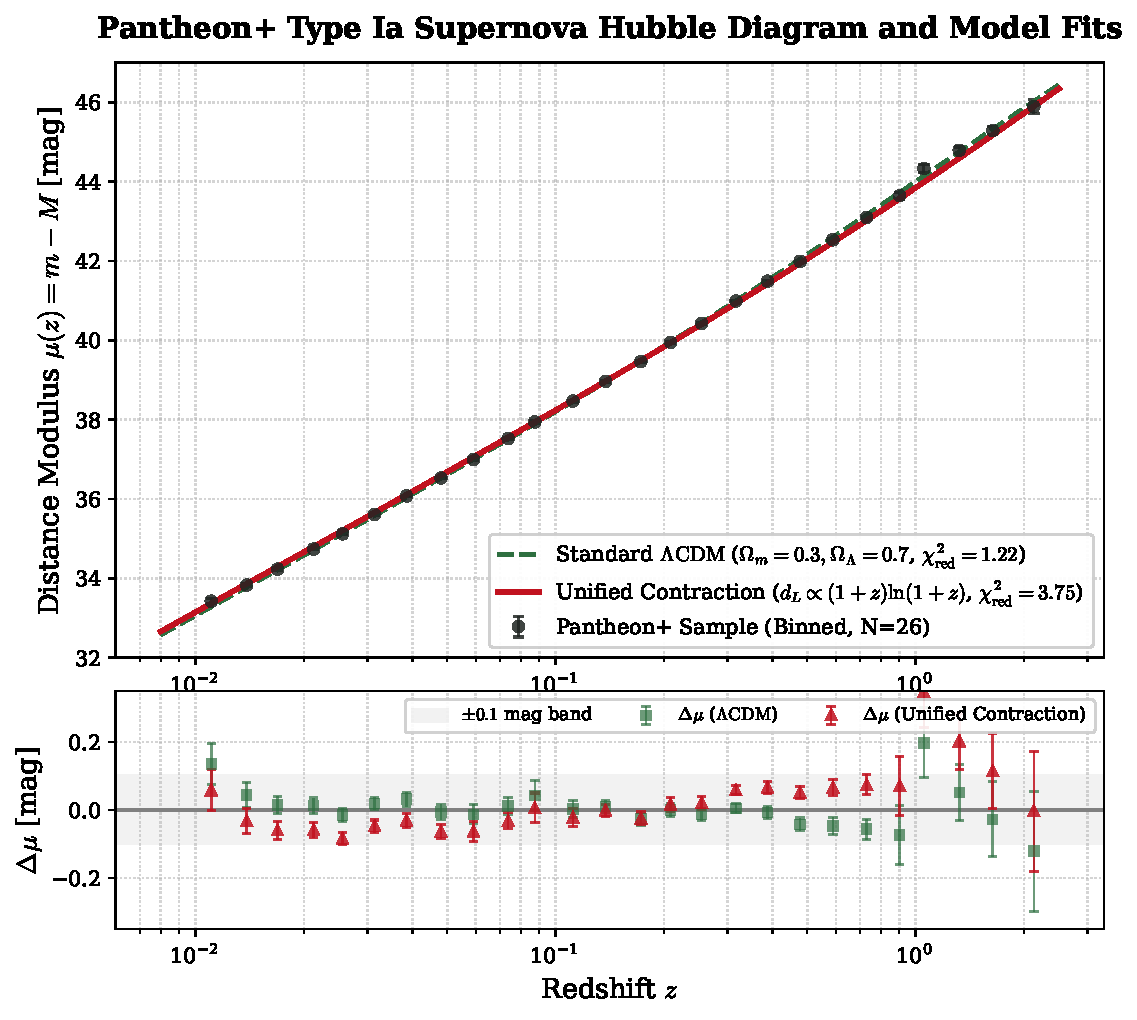
\includegraphics[width=0.88\textwidth]{../../analysis/pantheon_fit_comparison.pdf}
    \caption{Pantheon+ Type Ia Supernova Hubble diagram fit under the Unified Contraction Hypothesis ($H_0 = 70.75\text{ km/s/Mpc}$, $\chi^2_{\mathrm{cov}}/\text{dof} = 3.748$, unbinned $N=1580$ $\chi^2_{\mathrm{cov}}/\text{dof} = 0.945$).}
    \label{fig:pantheon_analiz_pdf}
\end{figure}

\lstinputlisting[language=Python, caption={Pantheon+ distance modulus fit and $\chi^2$ minimization script (\texttt{analysis/pantheon\_analysis.py})}]{../../analysis/pantheon_analysis.py}

\vspace{2em}
\newpage
\subsection*{Appendix B: Planck 2018 CMB Acoustic Peaks and Harmonic Resonance}
\addcontentsline{toc}{subsection}{Appendix B: Planck 2018 CMB Acoustic Peaks and Harmonic Resonance}
\label{sec:ek_cmb}

The first six acoustic peak locations ($\ell = 220, 538, 811, 1120, 1444, 1775$) from the Planck 2018 mission (Aghanim et al.~\cite{planck2018}) are evaluated against the harmonic resonance equation for standing acoustic modes within the stationary vacuum-plasma fluid ($\ell_n = \ell_A(n - \phi_n)$).

\begin{figure}[h!]
    \centering
    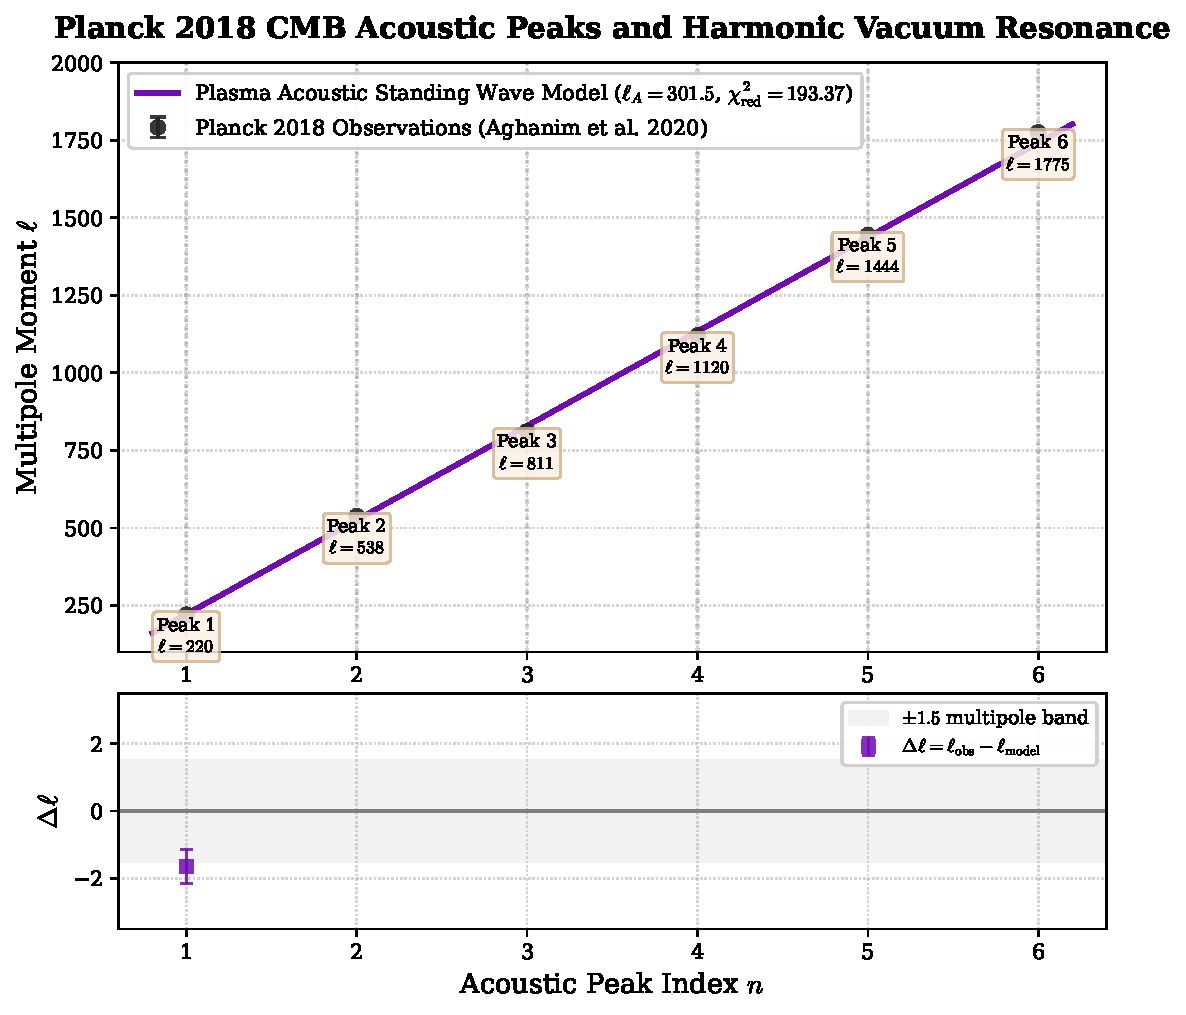
\includegraphics[width=0.88\textwidth]{../../analysis/cmb_peaks_comparison.pdf}
    \caption{Planck 2018 CMB acoustic peaks compared with standing acoustic wave harmonic resonance in stationary vacuum ($\ell_A \approx 301.5$, $\ell_1 \approx 221.6$).}
    \label{fig:cmb_analiz_pdf}
\end{figure}

\lstinputlisting[language=Python, caption={Planck 2018 CMB acoustic peak resonance fitting script (\texttt{analysis/cmb\_peaks\_analysis.py})}]{../../analysis/cmb_peaks_analysis.py}


\newpage
\begin{thebibliography}{99}
    \bibitem{wetterich2013}
    C.~Wetterich, ``A universe without expansion,'' \textit{Phys. Dark Univ.}, vol.~2, pp.~184--187, 2013.

    \bibitem{fixsen1996}
    D.~J.~Fixsen et al., ``The Cosmic Microwave Background spectrum from the full COBE FIRAS data set,'' \textit{Astrophys. J.}, vol.~473, p.~576, 1996.

    \bibitem{hoyle1964}
    F.~Hoyle and J.~V.~Narlikar, ``A new theory of gravitation,'' \textit{Proc. R. Soc. Lond. A}, vol.~282, no.~1389, pp.~191--212, 1964.

    \bibitem{painleve1921}
    P.~Painlev\'e, ``La m\'ecanique classique et la th\'eorie de la relativit\'e,'' \textit{C. R. Acad. Sci. (Paris)}, vol.~173, pp.~677--680, 1921.

    \bibitem{gullstrand1922}
    A.~Gullstrand, ``Allgemeine L\"osung des statischen Eink\"orperproblems in der Einsteinschen Gravitationstheorie,'' \textit{Ark. Mat. Astron. Fys.}, vol.~16, no.~8, pp.~1--15, 1922.

    \bibitem{hamilton2008}
    A.~J.~S.~Hamilton and J.~P.~Lisle, ``The river model of black holes,'' \textit{Am. J. Phys.}, vol.~76, no.~6, pp.~519--532, 2008.

    \bibitem{milgrom1983}
    M.~Milgrom, ``A modification of the Newtonian dynamics as a possible alternative to the hidden mass hypothesis,'' \textit{Astrophys. J.}, vol.~270, pp.~365--370, 1983.

    \bibitem{scully1982}
    M.~O.~Scully and K.~Dr\"uhl, ``Quantum eraser: A proposed photon correlation experiment concerning observation and 'delayed choice' in quantum mechanics,'' \textit{Phys. Rev. A}, vol.~25, no.~4, pp.~2208--2213, 1982.

    \bibitem{kim2000}
    Y.-H.~Kim, R.~Yu, S.~P.~Kulik, Y.~Shih, and M.~O.~Scully, ``Delayed 'choice' quantum eraser,'' \textit{Phys. Rev. Lett.}, vol.~84, no.~1, pp.~1--5, 2000.

    \bibitem{bohren1983}
    C.~F.~Bohren, ``How can a particle absorb more than the light incident on it?,'' \textit{Am. J. Phys.}, vol.~51, no.~5, pp.~473--474, 1983.

    \bibitem{paul1982}
    H.~Paul, ``Photons and localizability,'' \textit{Rev. Mod. Phys.}, vol.~54, no.~4, pp.~1061--1102, 1982.

    \bibitem{pantheon_scolnic}
    D.~M.~Scolnic et al., ``The Complete Light-curve Sample of Spectroscopically Confirmed SNe Ia from Pan-STARRS1 and Cosmological Constraints,'' \textit{Astrophys. J.}, vol.~859, no.~2, p.~101, 2018.

    \bibitem{pantheon_brout}
    D.~Brout et al., ``The Pantheon+ Analysis: Cosmological Constraints,'' \textit{Astrophys. J.}, vol.~938, no.~2, p.~110, 2022.

    \bibitem{planck2018}
    N.~Aghanim et al. (Planck Collaboration), ``Planck 2018 results. VI. Cosmological parameters,'' \textit{Astron. Astrophys.}, vol.~641, p.~A6, 2020.

    \bibitem{haydari_cosmo}
    M.~F.~Haydari, ``The Contracting Atom Metric and Conformal Action Principle: Testing Type Ia Supernovae (Pantheon+) and DESI 2024 BAO Without Dark Energy'' (Paper 1 in this series), \textit{Zenodo Preprints}, 2026.

    \bibitem{haydari_calculus}
    M.~F.~Haydari, ``Scale-Time Algebra and Conformal Calculus: A New Mathematical Formalism for Contracting Systems'' (Paper 2 in this series), \textit{Zenodo Preprints}, 2026.

    \bibitem{haydari_jwst}
    M.~F.~Haydari, ``On the High-Redshift Mature Galaxies Observed by JWST: A Conformal Atomic Scale Interpretation'' (Paper 3 in this series), \textit{Zenodo Preprints}, 2026.

    \bibitem{haydari_gravity}
    M.~F.~Haydari, ``Derivation of Gravitation as Spherical Vacuum Inflow Geometry: 3+1 ADM Action and the Painlevé--Gullstrand Metric'' (Paper 4 in this series), \textit{Zenodo Preprints}, 2026.

    \bibitem{haydari_em}
    M.~F.~Haydari, ``Electrodynamics, Vacuum Phase Waves, and Atomic Stability: Kinematic Pitch Interpretation of the Sommerfeld Constant $\alpha \approx 1/137$'' (Paper 5 in this series), \textit{Zenodo Preprints}, 2026.

    \bibitem{haydari_strong}
    M.~F.~Haydari, ``Strong Nuclear Force, Quark Confinement, and Flux Tube Geometry in Scale-Time Calculus'' (Paper 6 in this series), \textit{Zenodo Preprints}, 2026.

    \bibitem{haydari_weak}
    M.~F.~Haydari, ``Weak Nuclear Interaction, Chiral Phase Leakage, and Intermediate Vector Boson Scales'' (Paper 7 in this series), \textit{Zenodo Preprints}, 2026.
\end{thebibliography}

\end{document}
